\section{Introduction}

In modular robotic systems, coordination among a group of modules often relies on the existence of a common notion of time. For instance, in the conveyance surface presented in Section~\ref{section:context:conveyance-surface}, modules cooperate to convey the object using distributed real-time control. They have to remain synchronized in order to satisfy timing constraints, otherwise the object may get out of the trajectory, hit obstacles or fall off the surface. The next section presents another interesting application, the distributed bitmap scroller, in which every module is a pixel and the modules collaboratively scroll a bitmap in a synchronous way. Coordination of the modules requires synchronized clocks. More generally, many applications that involve distributed control and actuators need a common notion of time.

Modules can share a common timing signal through dedicated pins, but this requires a specific hardware design. In this chapter, we consider a system without a global clock signal. Every module has its own notion of time provided by its own hardware clock. Since common hardware clocks are imperfect, local clocks tend to run at slightly different and variable frequencies, drifting apart from each other over time. Consequently, a distributed time synchronization is necessary to keep the local clock of each module synchronized to a global timescale. The offset of two clocks denotes the time difference between them, whereas the skew between two clocks denotes their frequency difference.

Network-wide synchronization protocols aim to keep a small offset between local clocks and a global reference time. In most of the existing protocols, devices exchange timestamped messages in order to estimate the current global time. Since time keeps going during communications, modules have to correctly compensate for network delays in order to evaluate the current global time upon reception of synchronization messages. Although it is non-trivial to accurately estimate communication delays, especially in the presence of unpredictable delays (due, for example, to queueing or retransmissions), it is crucial in order to achieve high-precision performance.

The contribution of this chapter is to propose the Modular Robot Time Protocol (MRTP), a network-wide time synchronization protocol for modular robots with neighbor-to-neighbor communications. MRTP is intended to synchronize fairly stable systems where changes in the network topology, due for instance to module mobility, or potential module or link failures, are infrequent. We assume that every module has a local clock, which can be low-precision and low-resolution, typically in the order of the millisecond. Furthermore, modules can use low communication bitrates (e.g, 38.4 kbit/s). In addition, we assume that modules can timestamp messages at the data-link layer. Such a low resolution, low precision and high communication latency make accurate synchronization challenging. First, the local time cannot be accurately read. Second, it is hard to accurately compensate for network delays if they are not negligible and, at the same time, only roughly measurable. Third, clock skew and clock instability may not be negligible during high-latency (multi-hop) communications.

To the best of our knowledge, MRTP is the first protocol for modular robots that provides an accurate low-skew global timescale without dedicated hardware. Our protocol combines new ideas with existing methods proposed in the domains of computer networks and wireless sensor networks. In our protocol, a dynamically elected central module periodically broadcasts the current global time along the edges of a spanning tree. Placing the time master close to the center of the system reduces the time of the synchronization phases and increases the overall precision as cumulative estimations are made every hop. The method to compensate for communication delays is carefully chosen, depending on the target systems. In Blinky Blocks systems, we use data-link layer timestamping and predictions of the transfer time (as defined in Section~\ref{section:time-sync:msg-decomposition}) to correctly compensate for network delays. A module gets synchronized by a single timestamped message from its parent one level higher in the tree, incurring little message overhead. Furthermore, modules use linear regression to compensate for clock skew.

We implemented our protocol and evaluated it on the Blinky Blocks system, both on hardware\footnote{The source code of MRTP is included in the Blinky Blocks firmware, available online at \url{https://github.com/claytronics/oldbb}}\footnote{Some examples of MRTP running on the Blinky Blocks platform are available online in video at \url{https://youtu.be/66D12ESGc98} and \url{https://youtu.be/X6QzivsmJBo}} and in the VisibleSim simulator\footnote{The source code of VisibleSim and the applications written for the evaluation of our protocol are available online at: \VisibleSimUrl{}} (see Section~\ref{section:context:environment}). We show that MRTP is able to manage systems composed of up to 27,775 Blinky Blocks. Furthermore, experimental results show that MRTP is capable of successfully maintaining a Blinky Blocks system synchronized to a few milliseconds, using few network resources at runtime, although the Blinky Blocks use 38.4 kbit/s communications and are equipped with very low accuracy (10,000 parts per million (ppm)) and poor resolution (1 millisecond) clocks.

The rest of this chapter is organized as follows. Section~\ref{section:time-sync:scroller} presents a practical application of MRTP in order to motivate our work and to show its necessity. Section~\ref{section:time-sync:related-works} offers an overview of the existing time synchronization protocols. Section~\ref{section:time-sync:model} details the system model and assumptions. Section~\ref{section:time-sync:protocol} describes MRTP. Section~\ref{section:time-sync:target} describes the technical characteristics of the  Blinky Blocks, i.e., the target platform. Section~\ref{section:time-sync:evaluation} presents experimental results. Section~\ref{section:time-sync:conclusion} concludes our work.

\section{Example of Application: The Distributed Bitmap Scroller}
\label{section:time-sync:scroller}

This section presents the distributed bitmap scroller application\footnote{A video of a distributed bitmap scroller made from 72 Blinky Blocks synchronized using MRTP is available online at \url{https://youtu.be/66D12ESGc98}}. In this application originally imagined by Beno{\^i}t Piranda, every module represents a pixel and the modules cooperatively scroll a text (here \say{Femto-st}) using color changes. The scroller is extensible and robust to system split and merge. Figure~\ref{fig:time-sync:bitmap-scroller} shows a distributed bitmap scroller made from 72 Blinky Blocks. We first present our implementation and then discuss the need for global time synchronization.

{
	\newcommand{\subFigureWidth}{0.32\linewidth}
	\begin{figure}[h!]
		\centering			
		\small
		\begin{tabular}{c c c}
			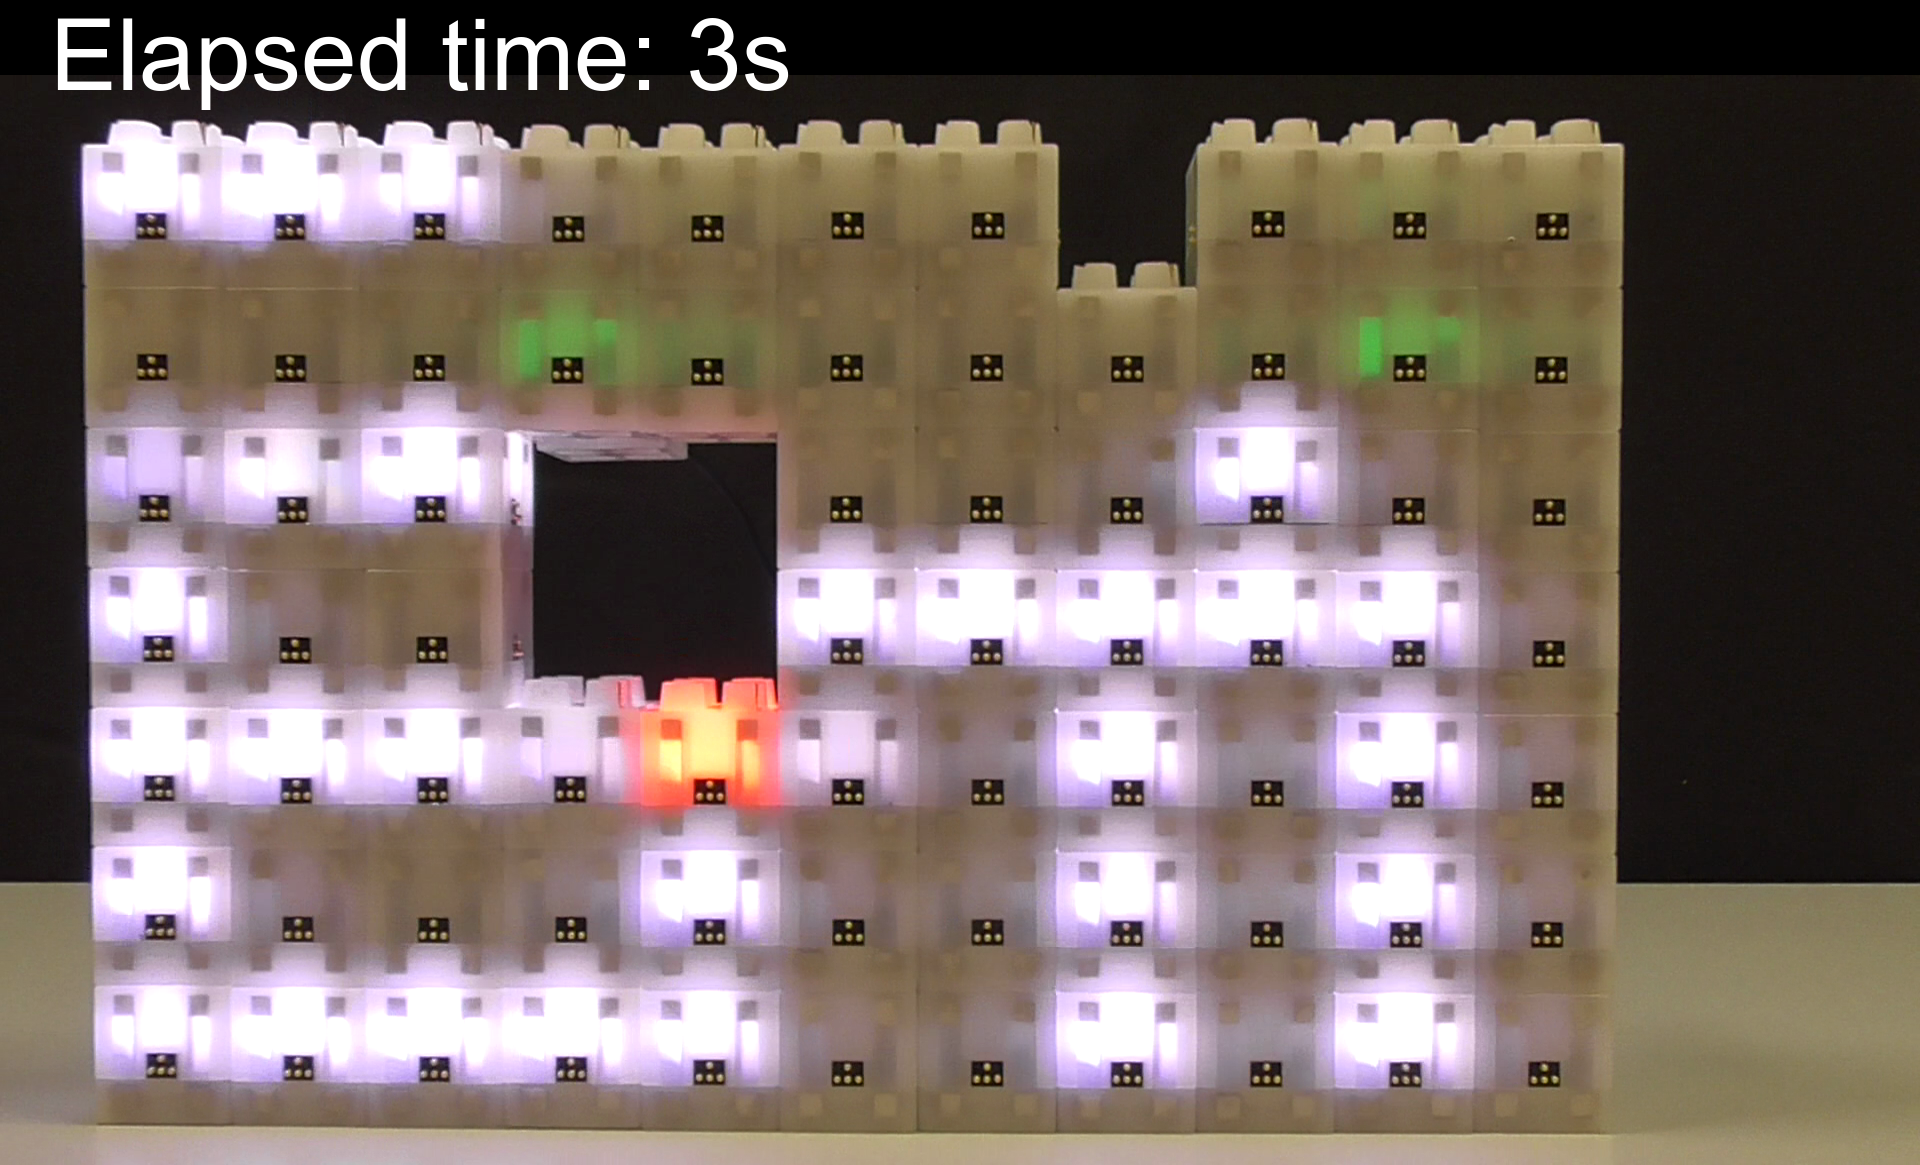
\includegraphics[width=\subFigureWidth]{images/time-synchronization/scroller/sync_3s}  &
			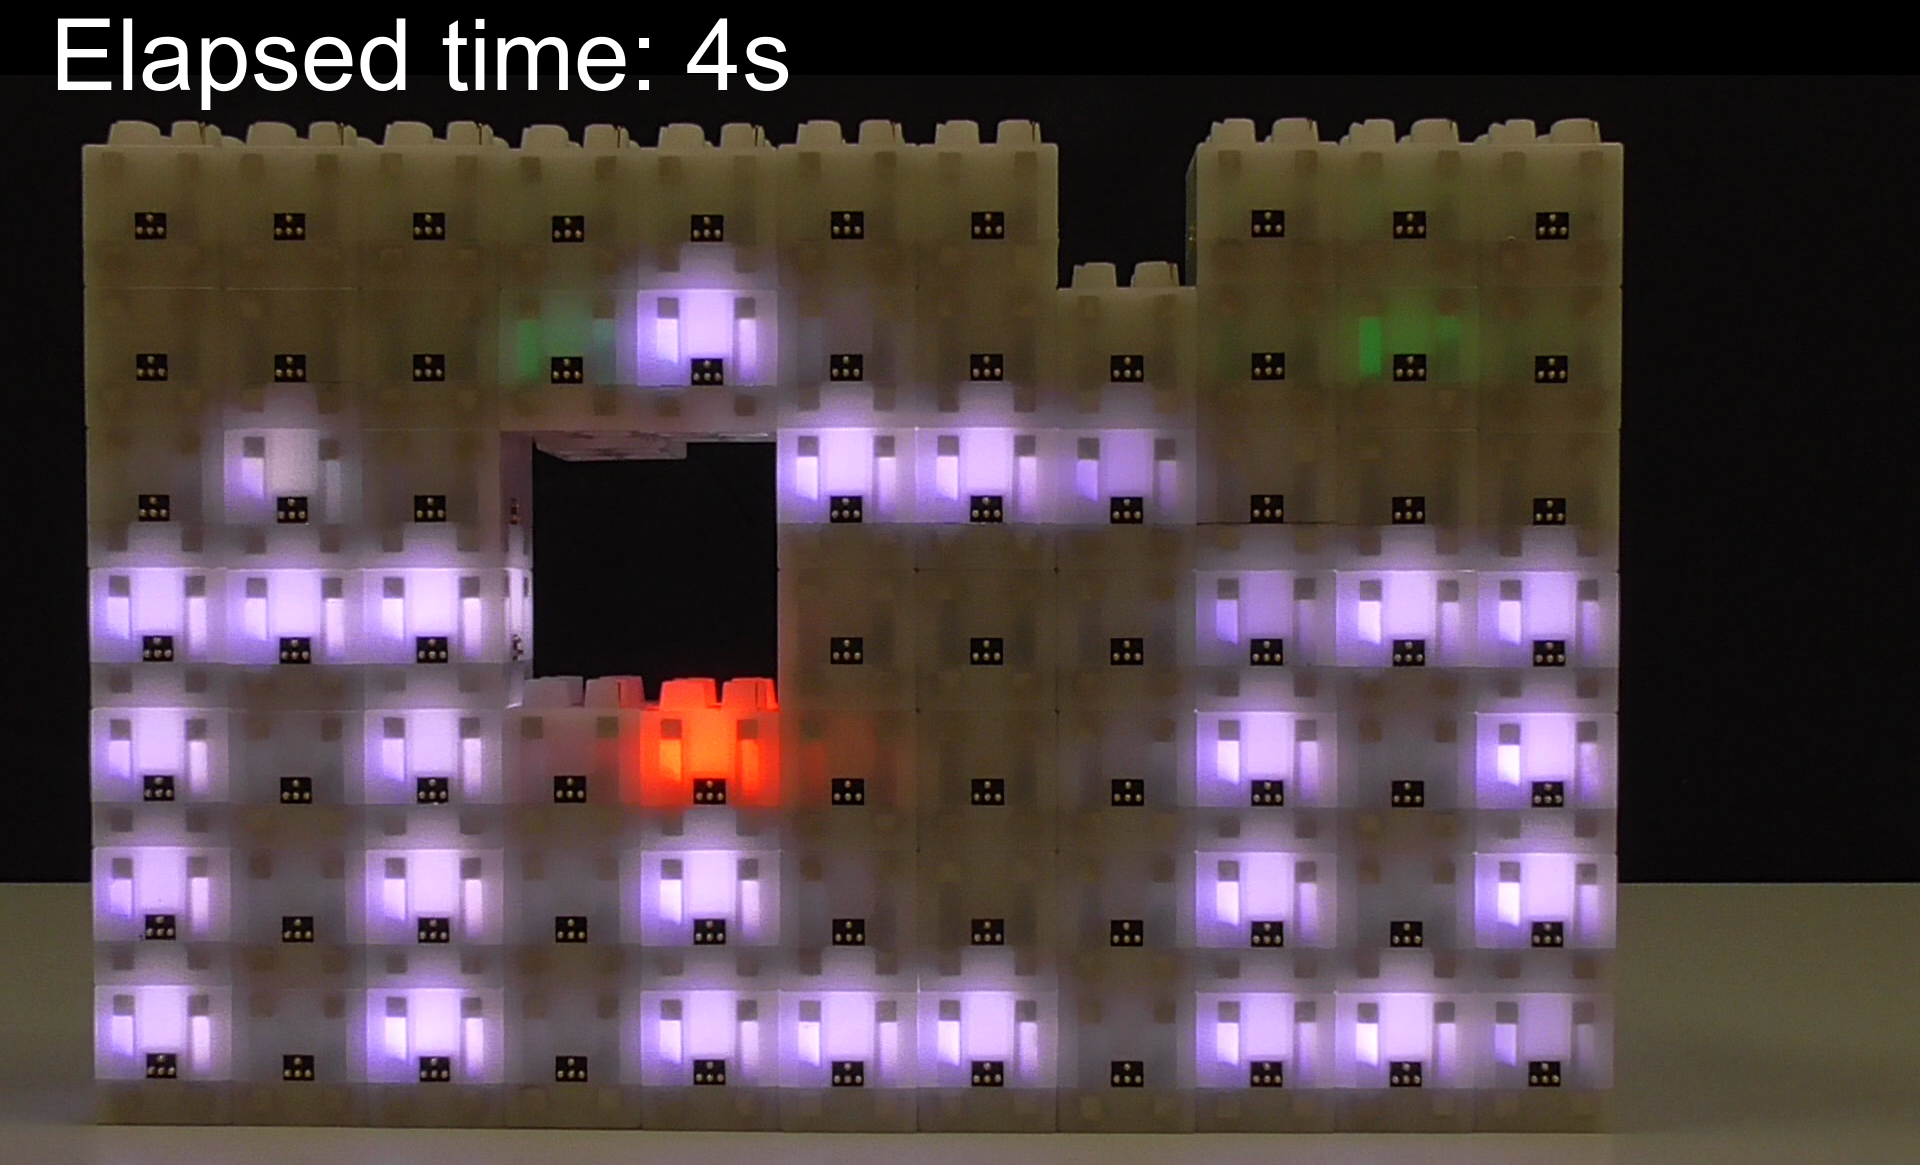
\includegraphics[width=\subFigureWidth]{images/time-synchronization/scroller/sync_4s} & 
			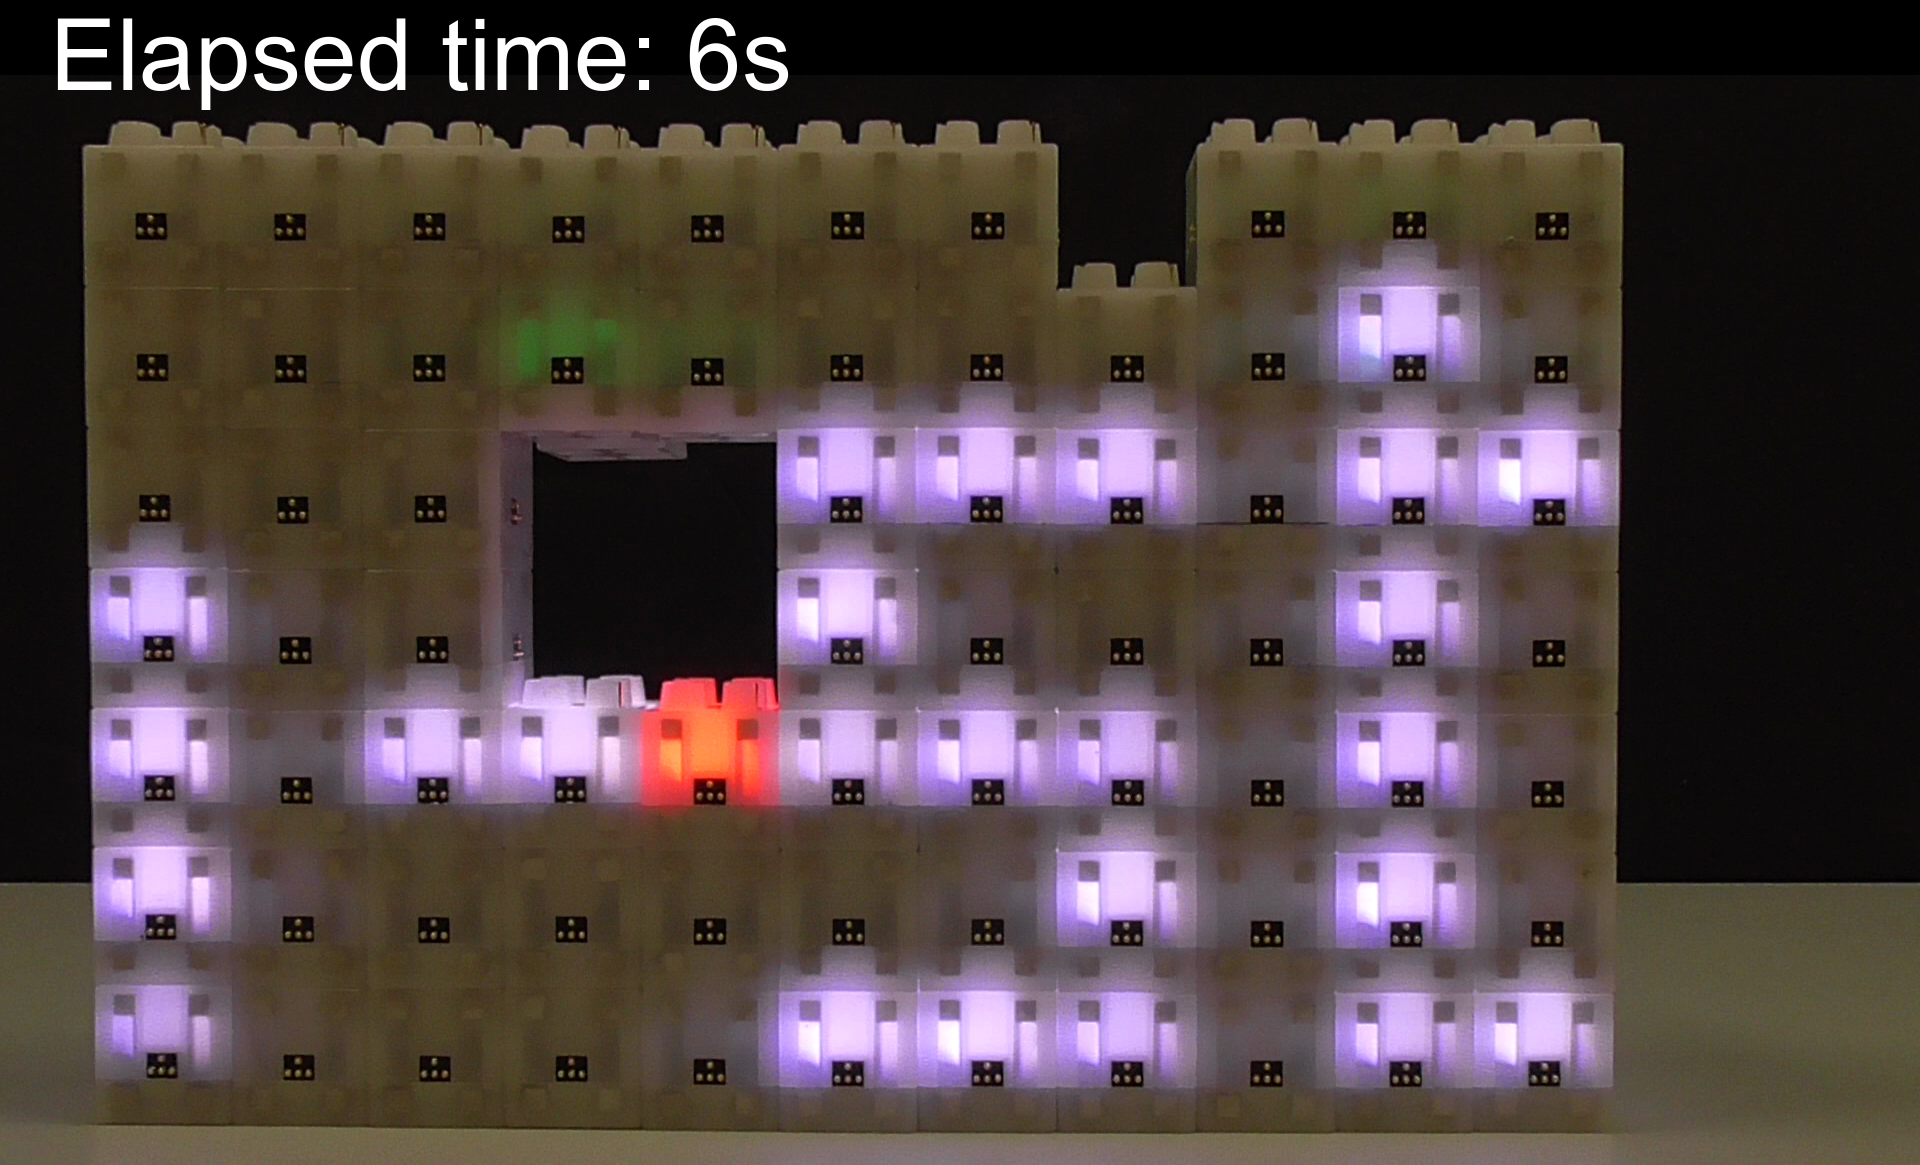
\includegraphics[width=\subFigureWidth]{images/time-synchronization/scroller/sync_6s}\\
			
			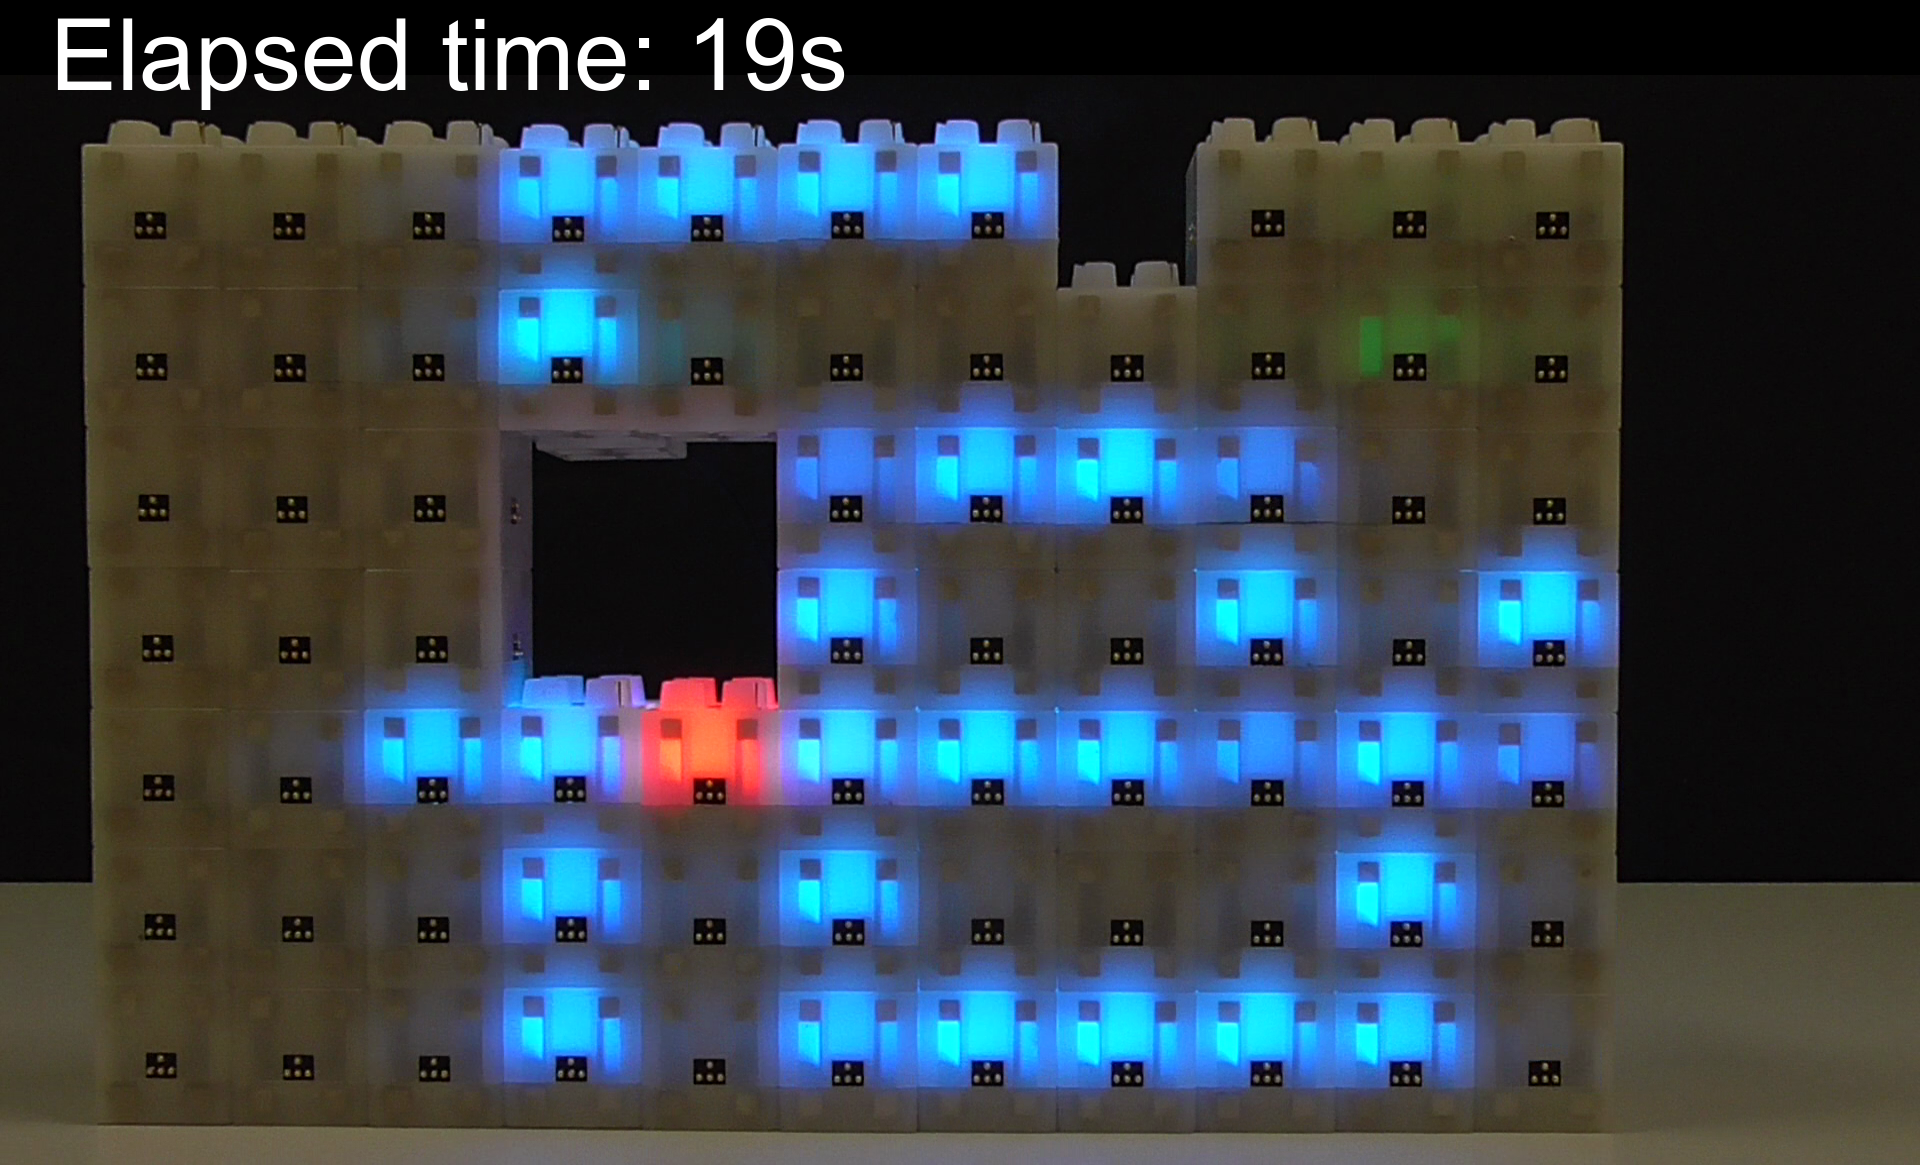
\includegraphics[width=\subFigureWidth]{images/time-synchronization/scroller/sync_19s}  &
			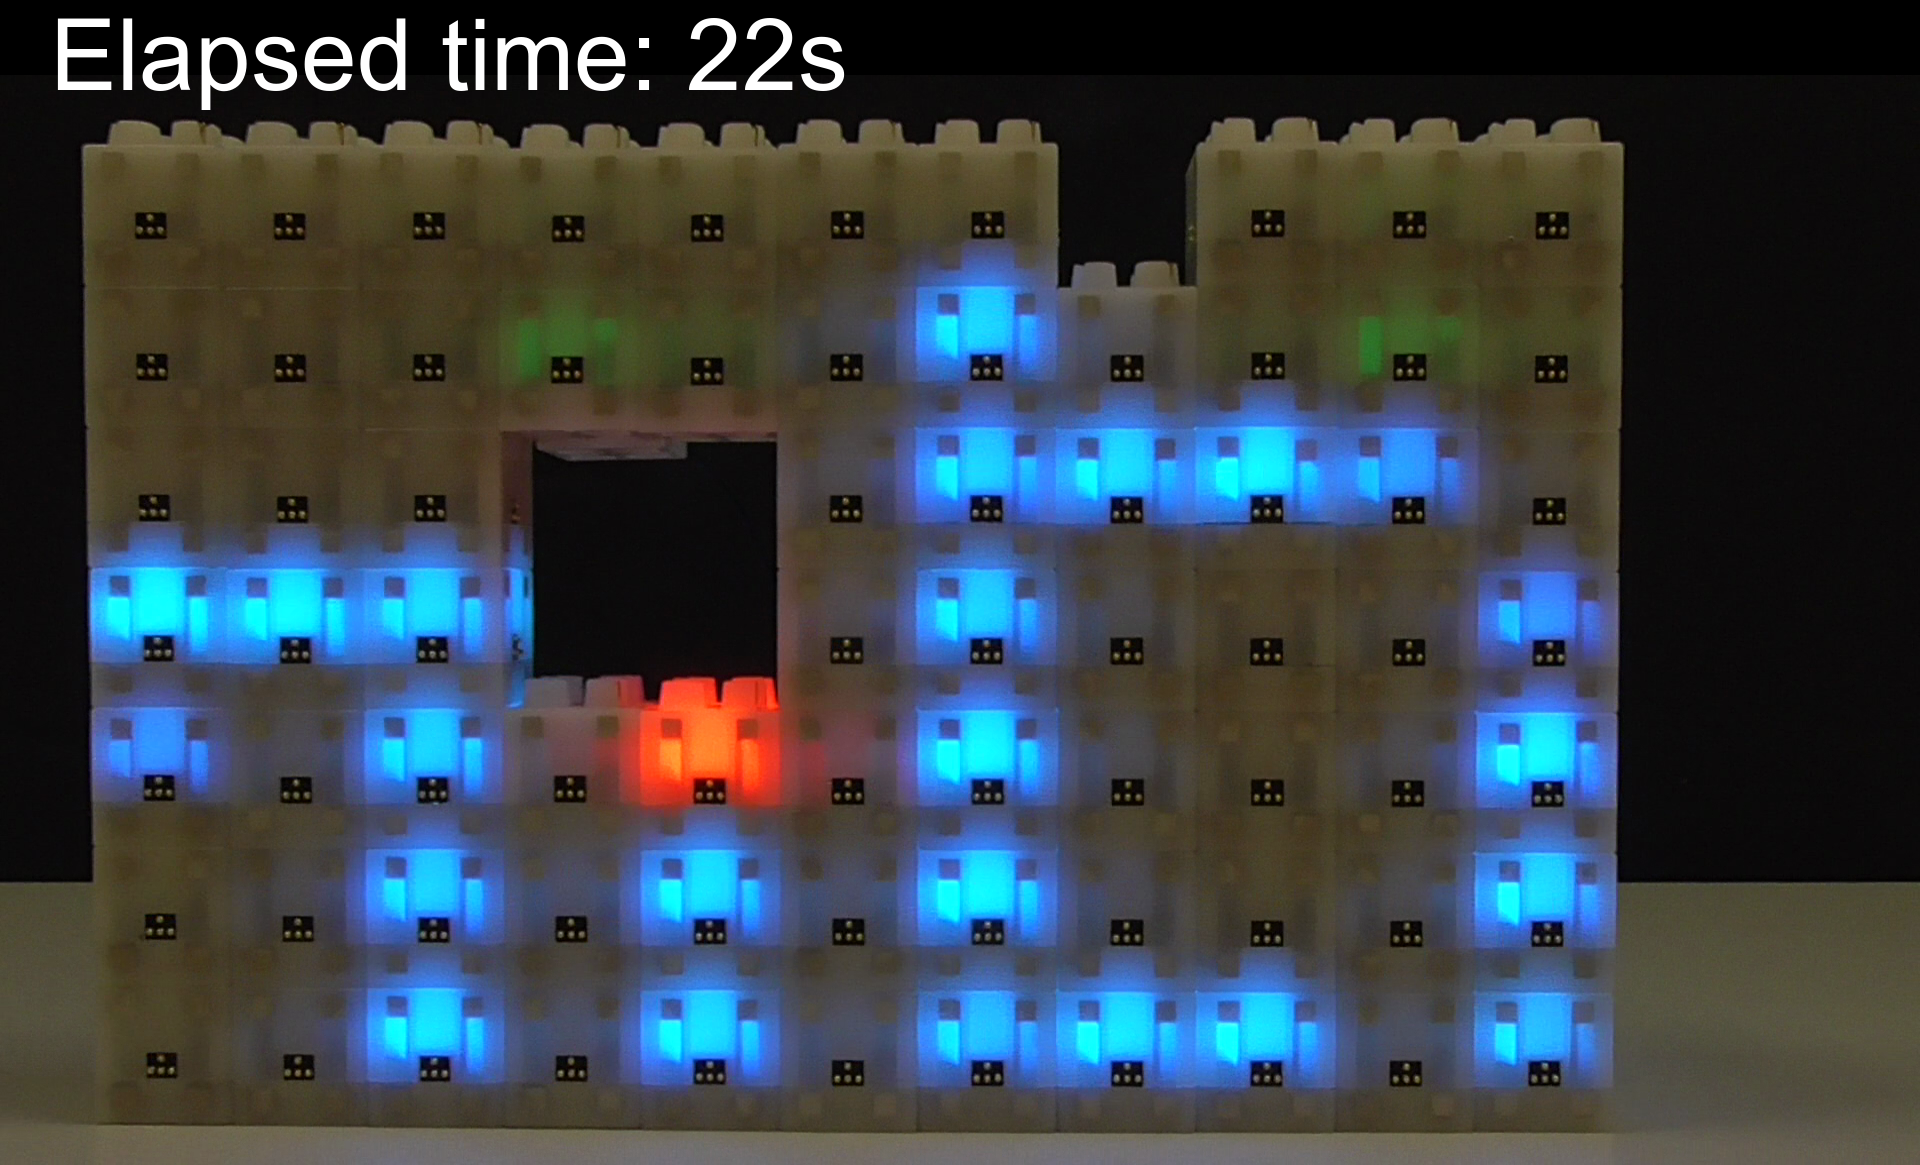
\includegraphics[width=\subFigureWidth]{images/time-synchronization/scroller/sync_22s} &
			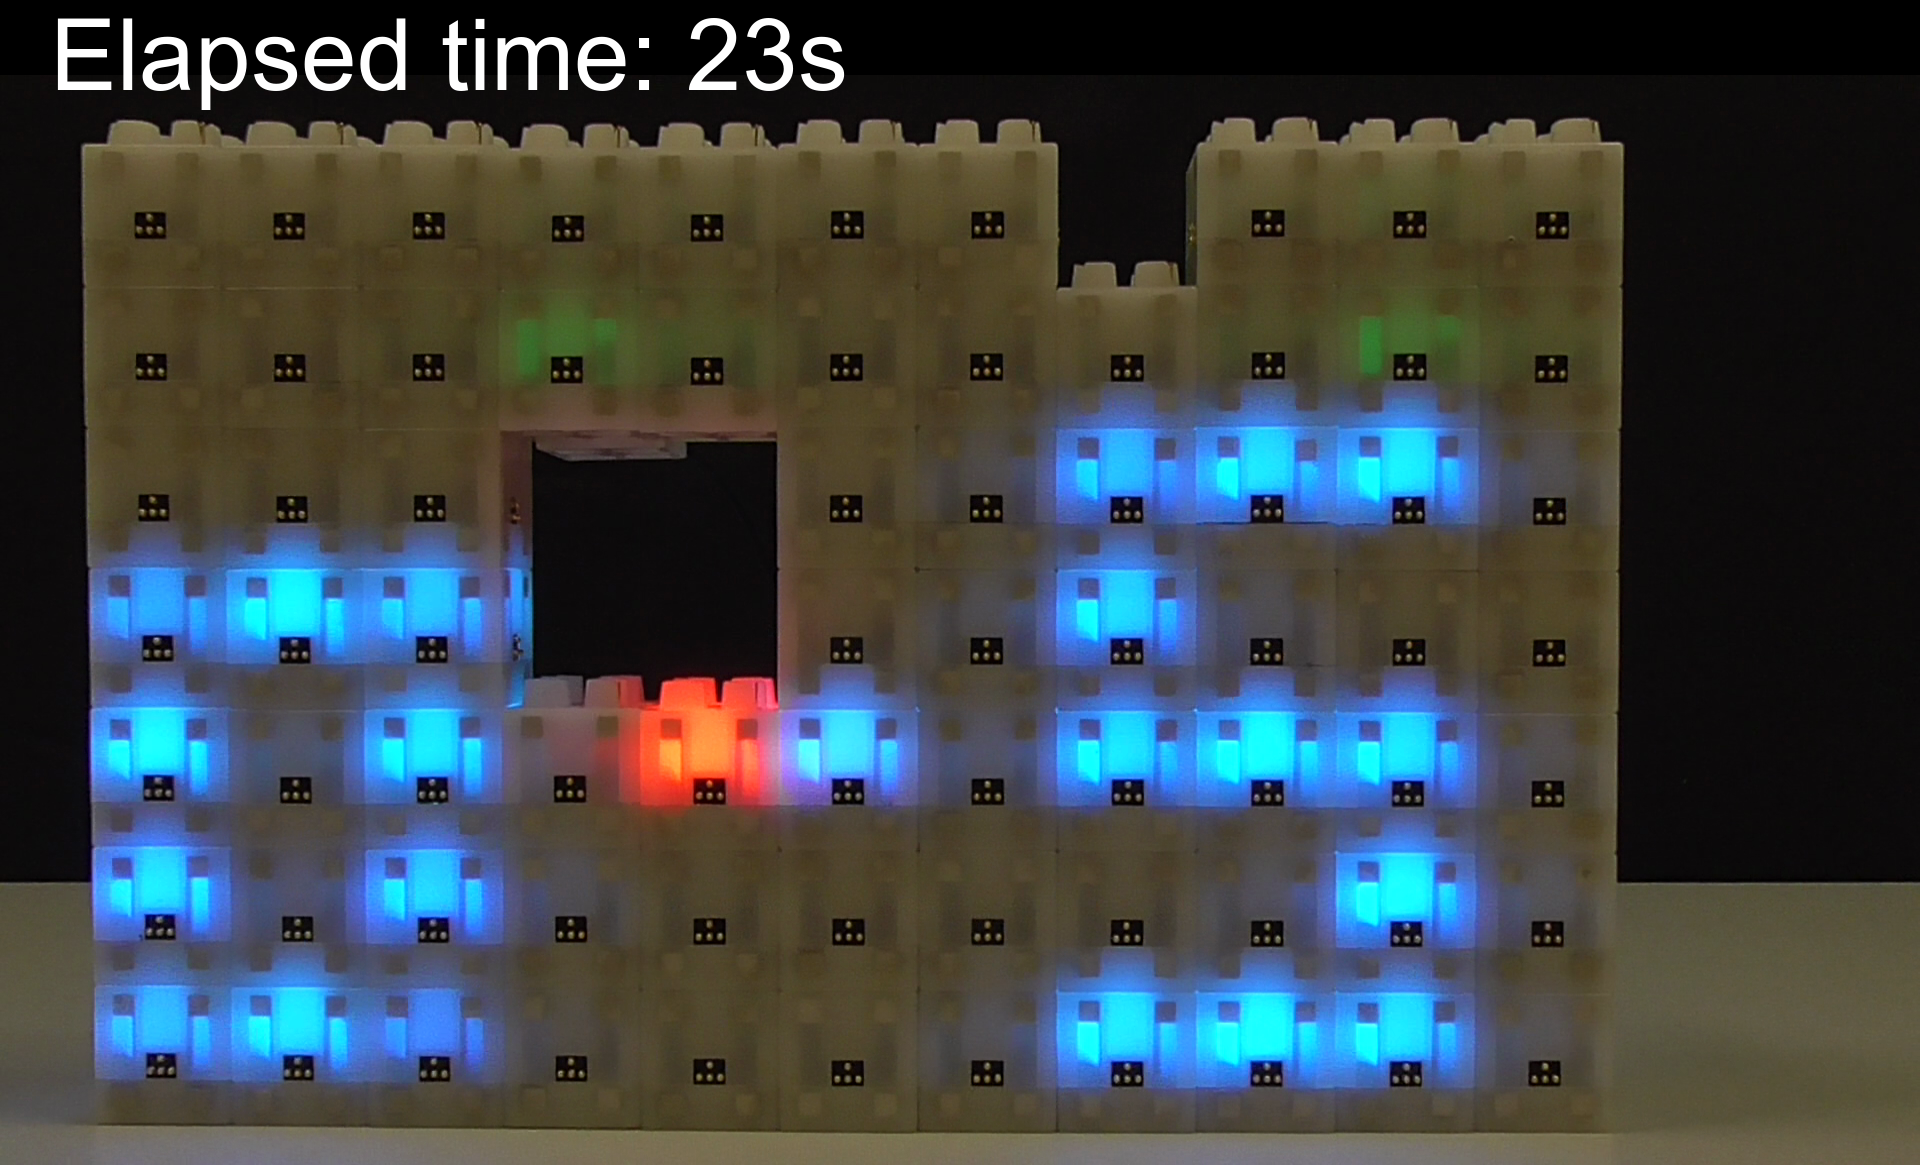
\includegraphics[width=\subFigureWidth]{images/time-synchronization/scroller/sync_23s}  \\
			
			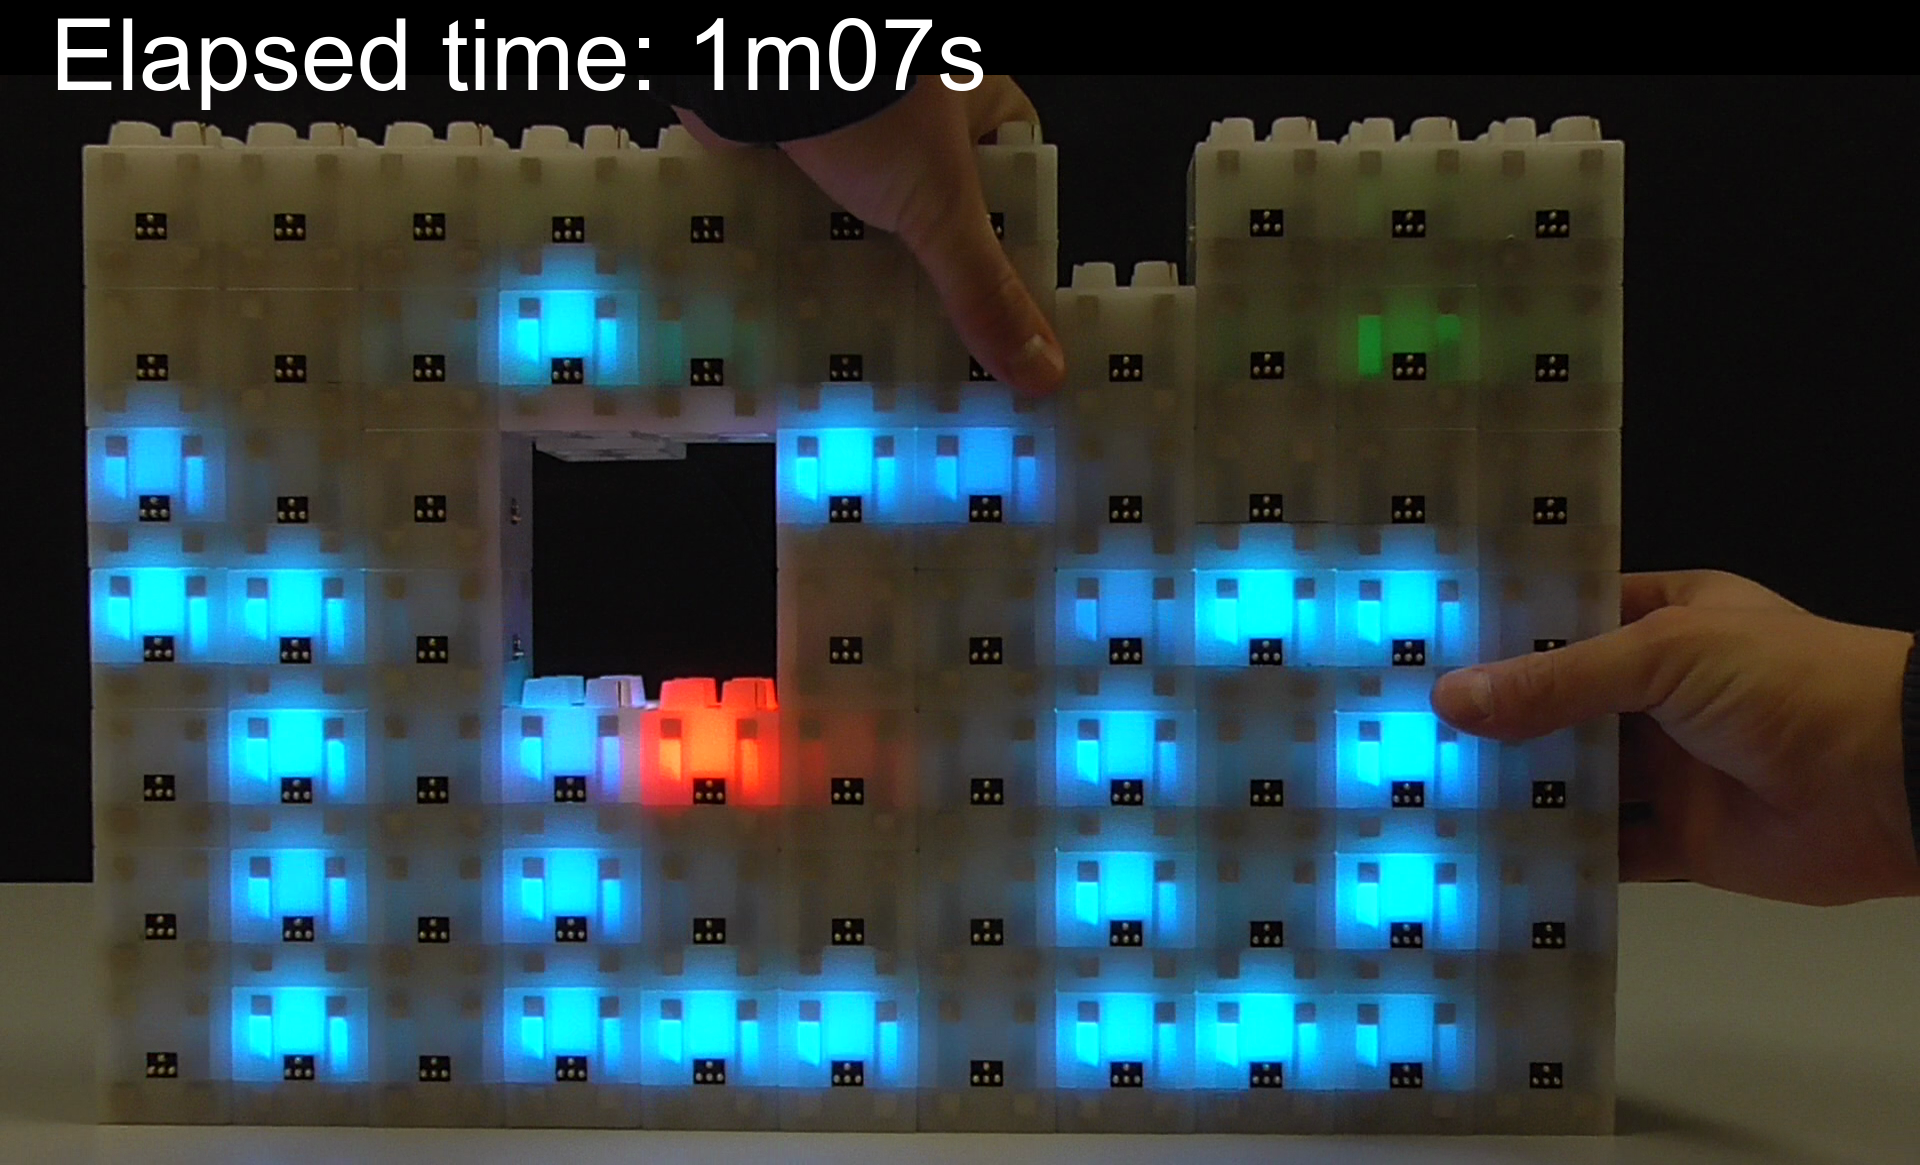
\includegraphics[width=\subFigureWidth]{images/time-synchronization/scroller/sync_1m07s} &
			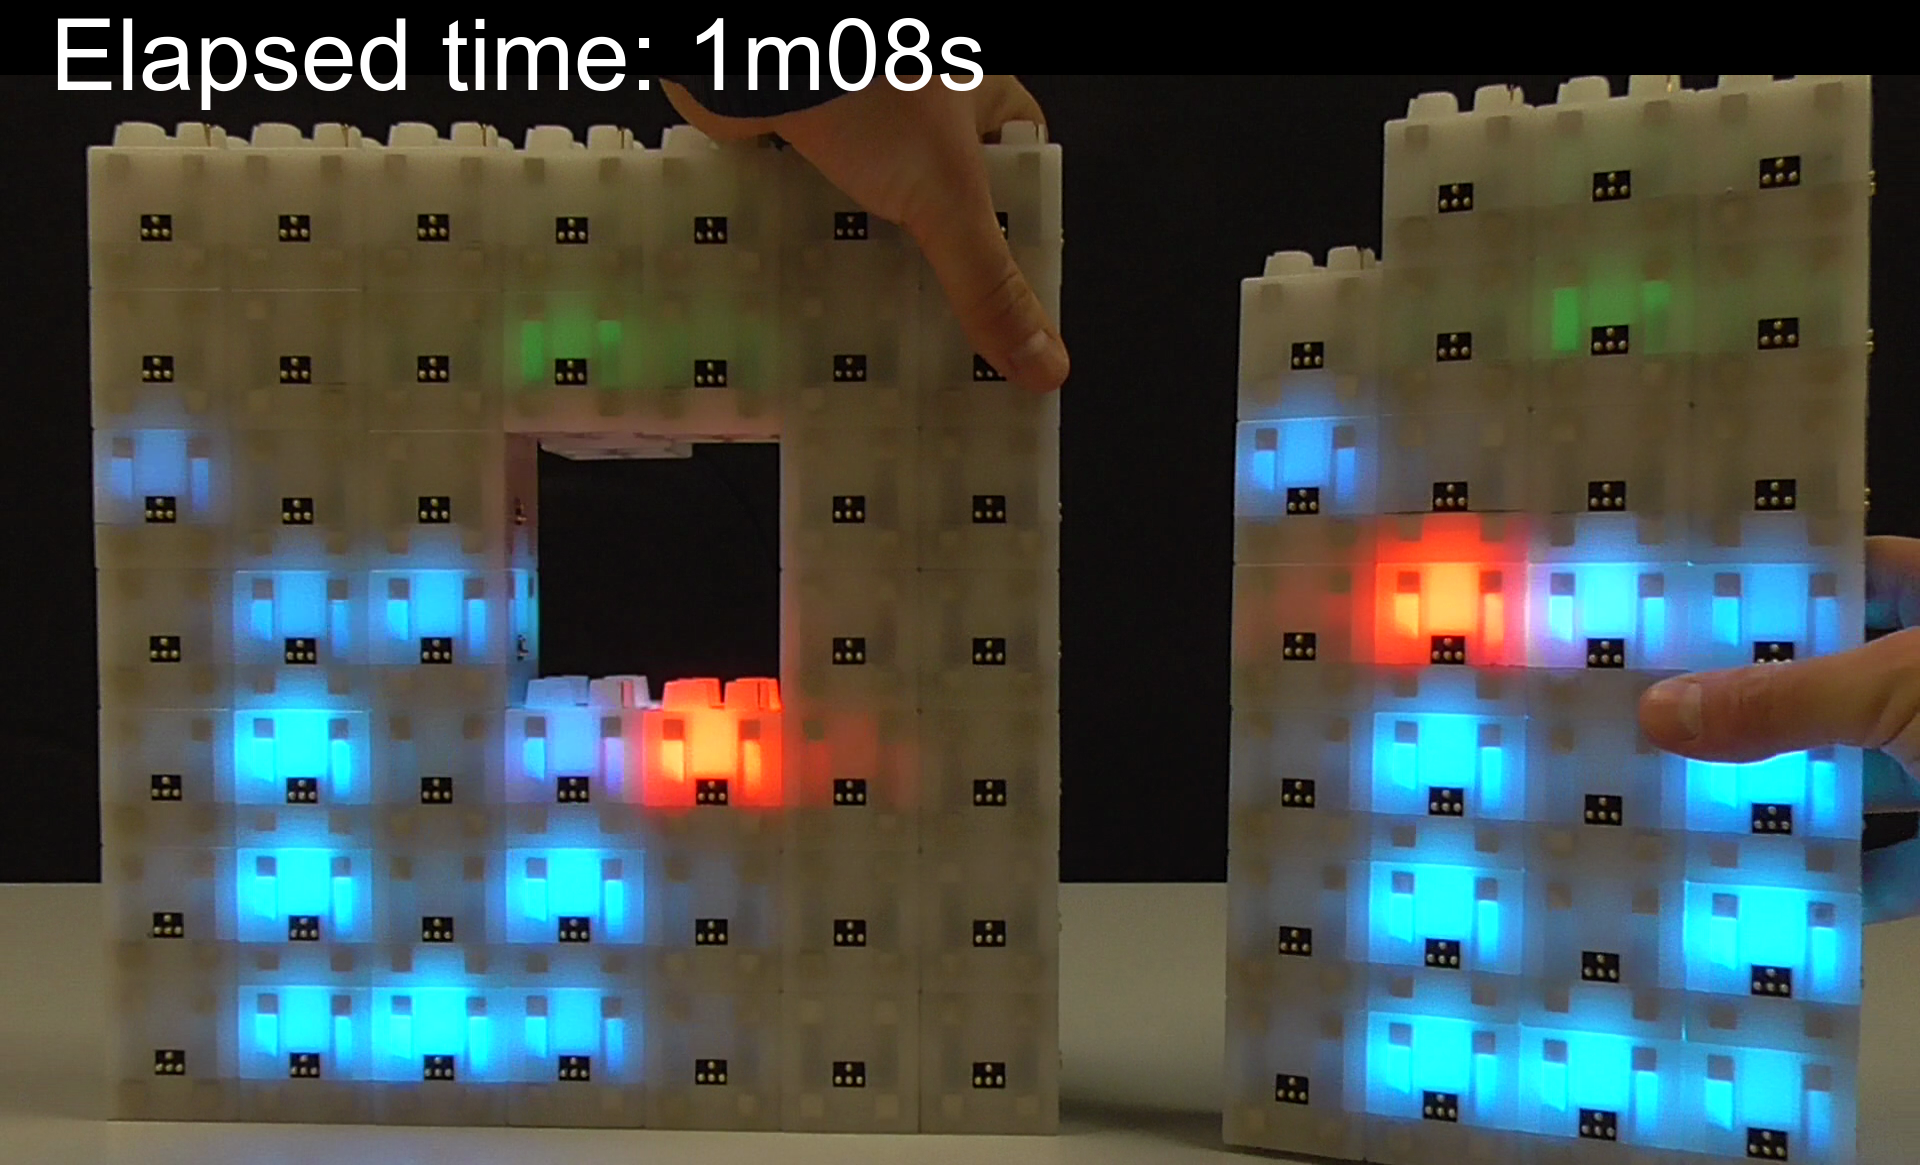
\includegraphics[width=\subFigureWidth]{images/time-synchronization/scroller/sync_1m08s} &
			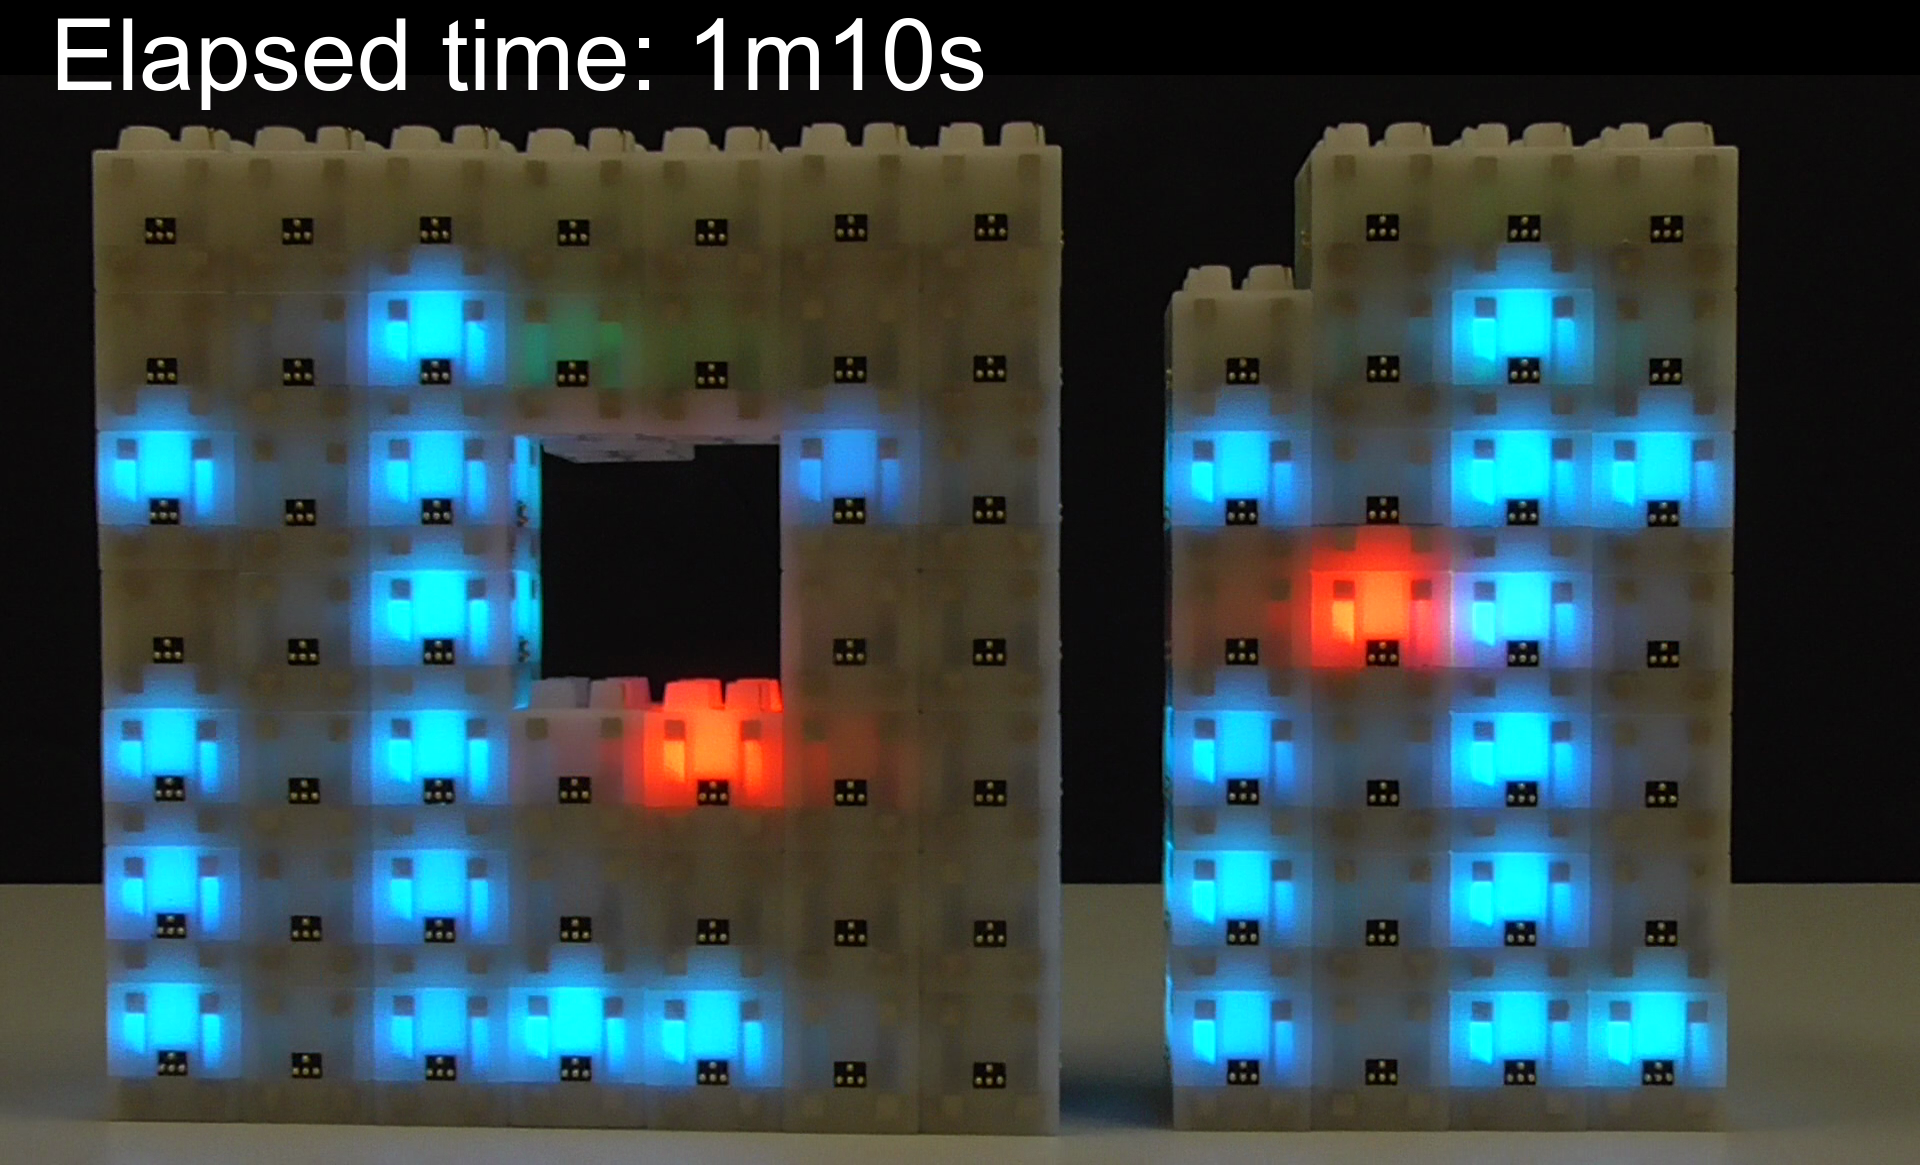
\includegraphics[width=\subFigureWidth]{images/time-synchronization/scroller/sync_1m10s} \\
			
			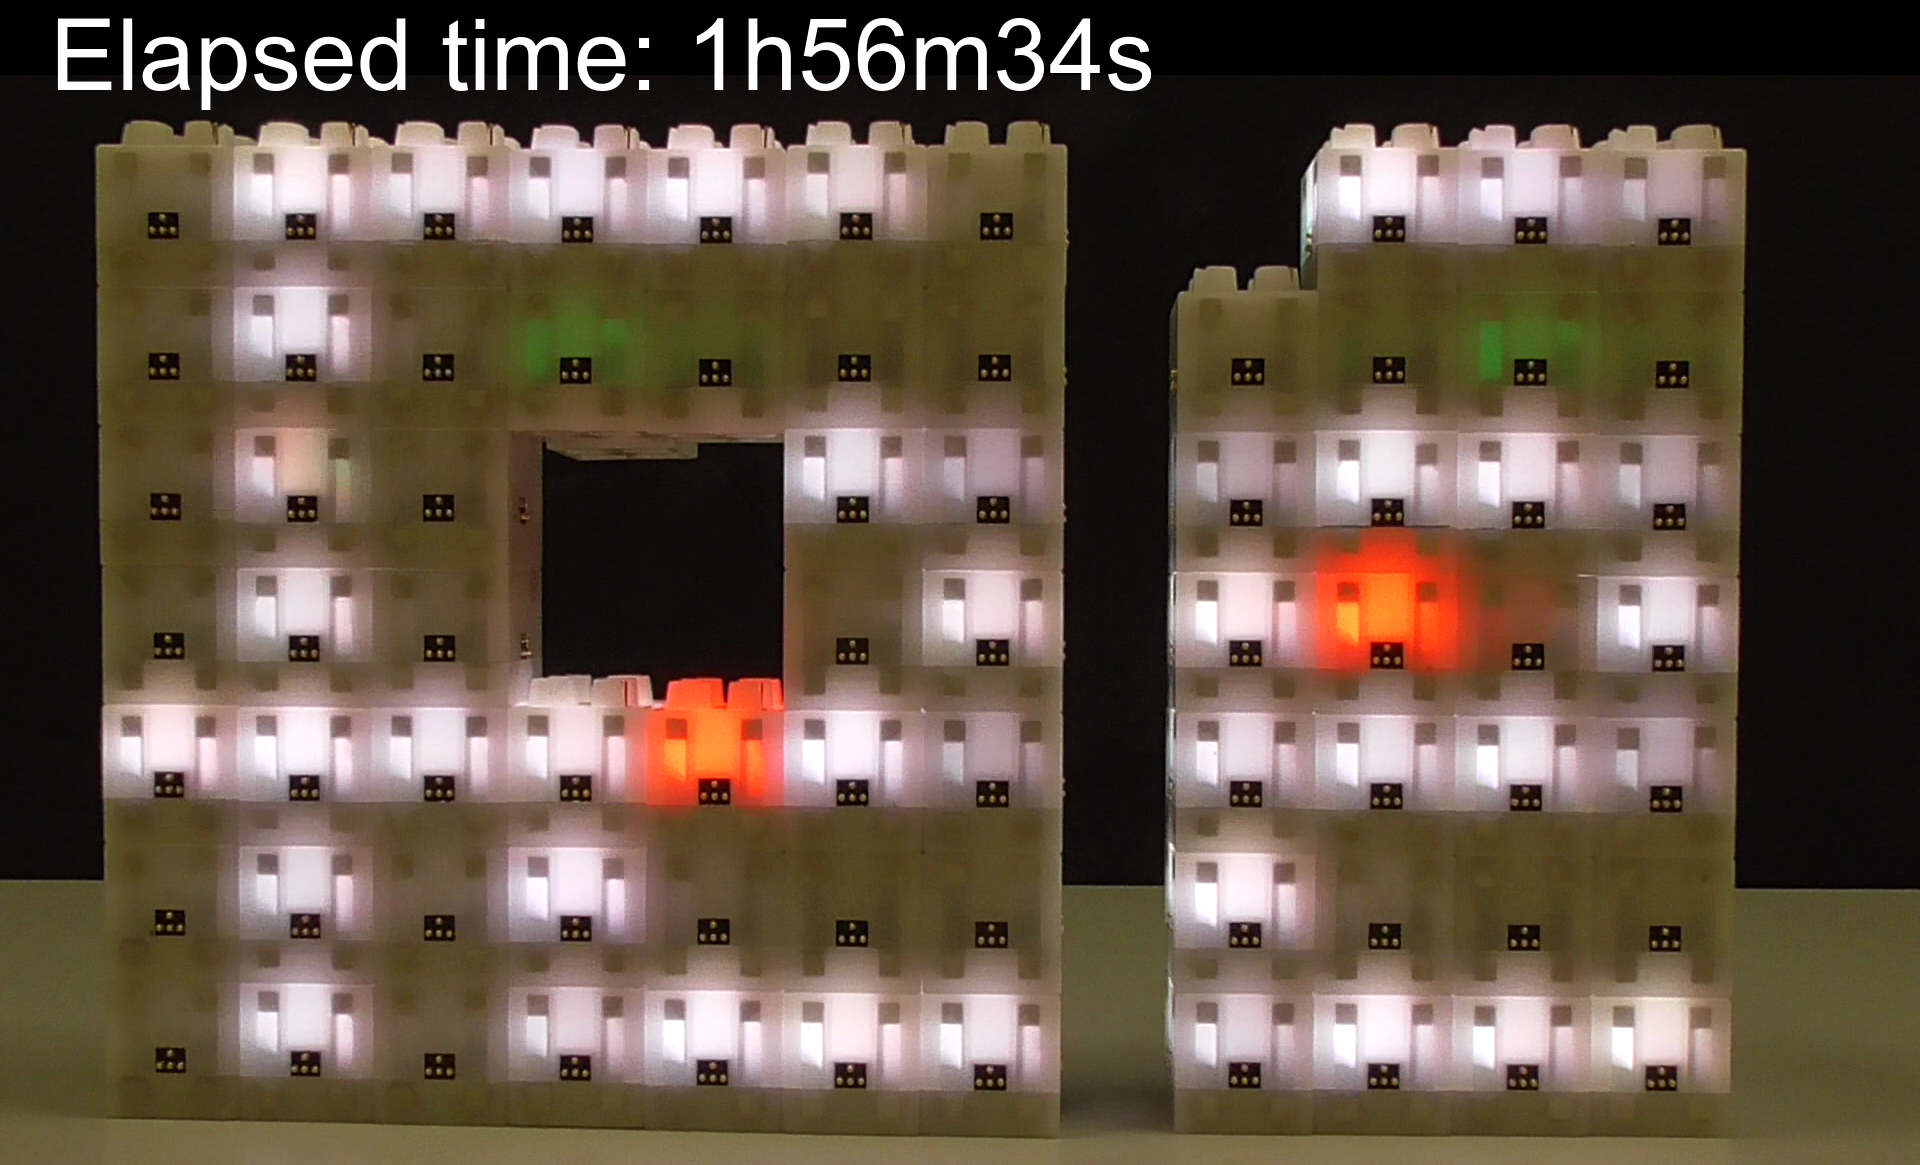
\includegraphics[width=\subFigureWidth]{images/time-synchronization/scroller/sync_1h56m34s} &
			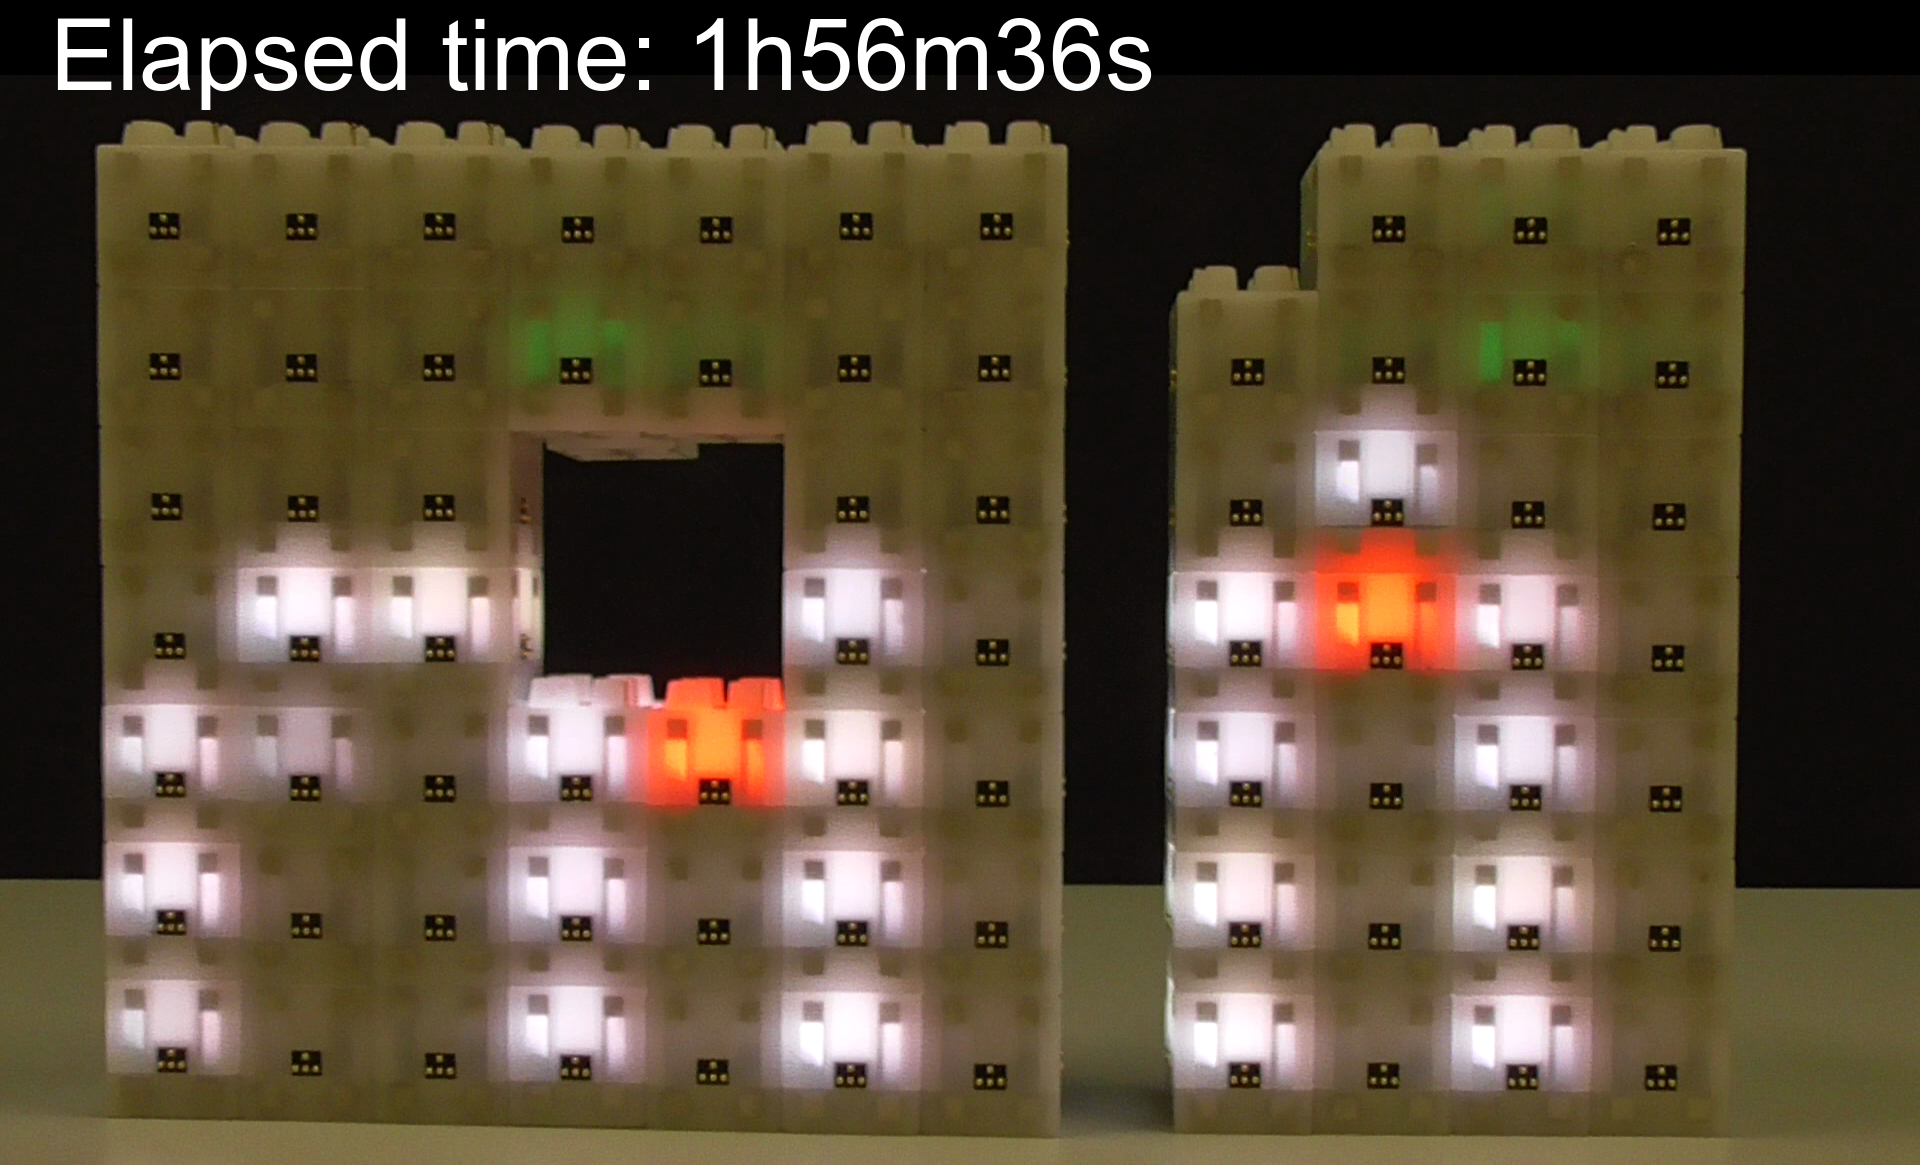
\includegraphics[width=\subFigureWidth]{images/time-synchronization/scroller/sync_1h56m36s} &
			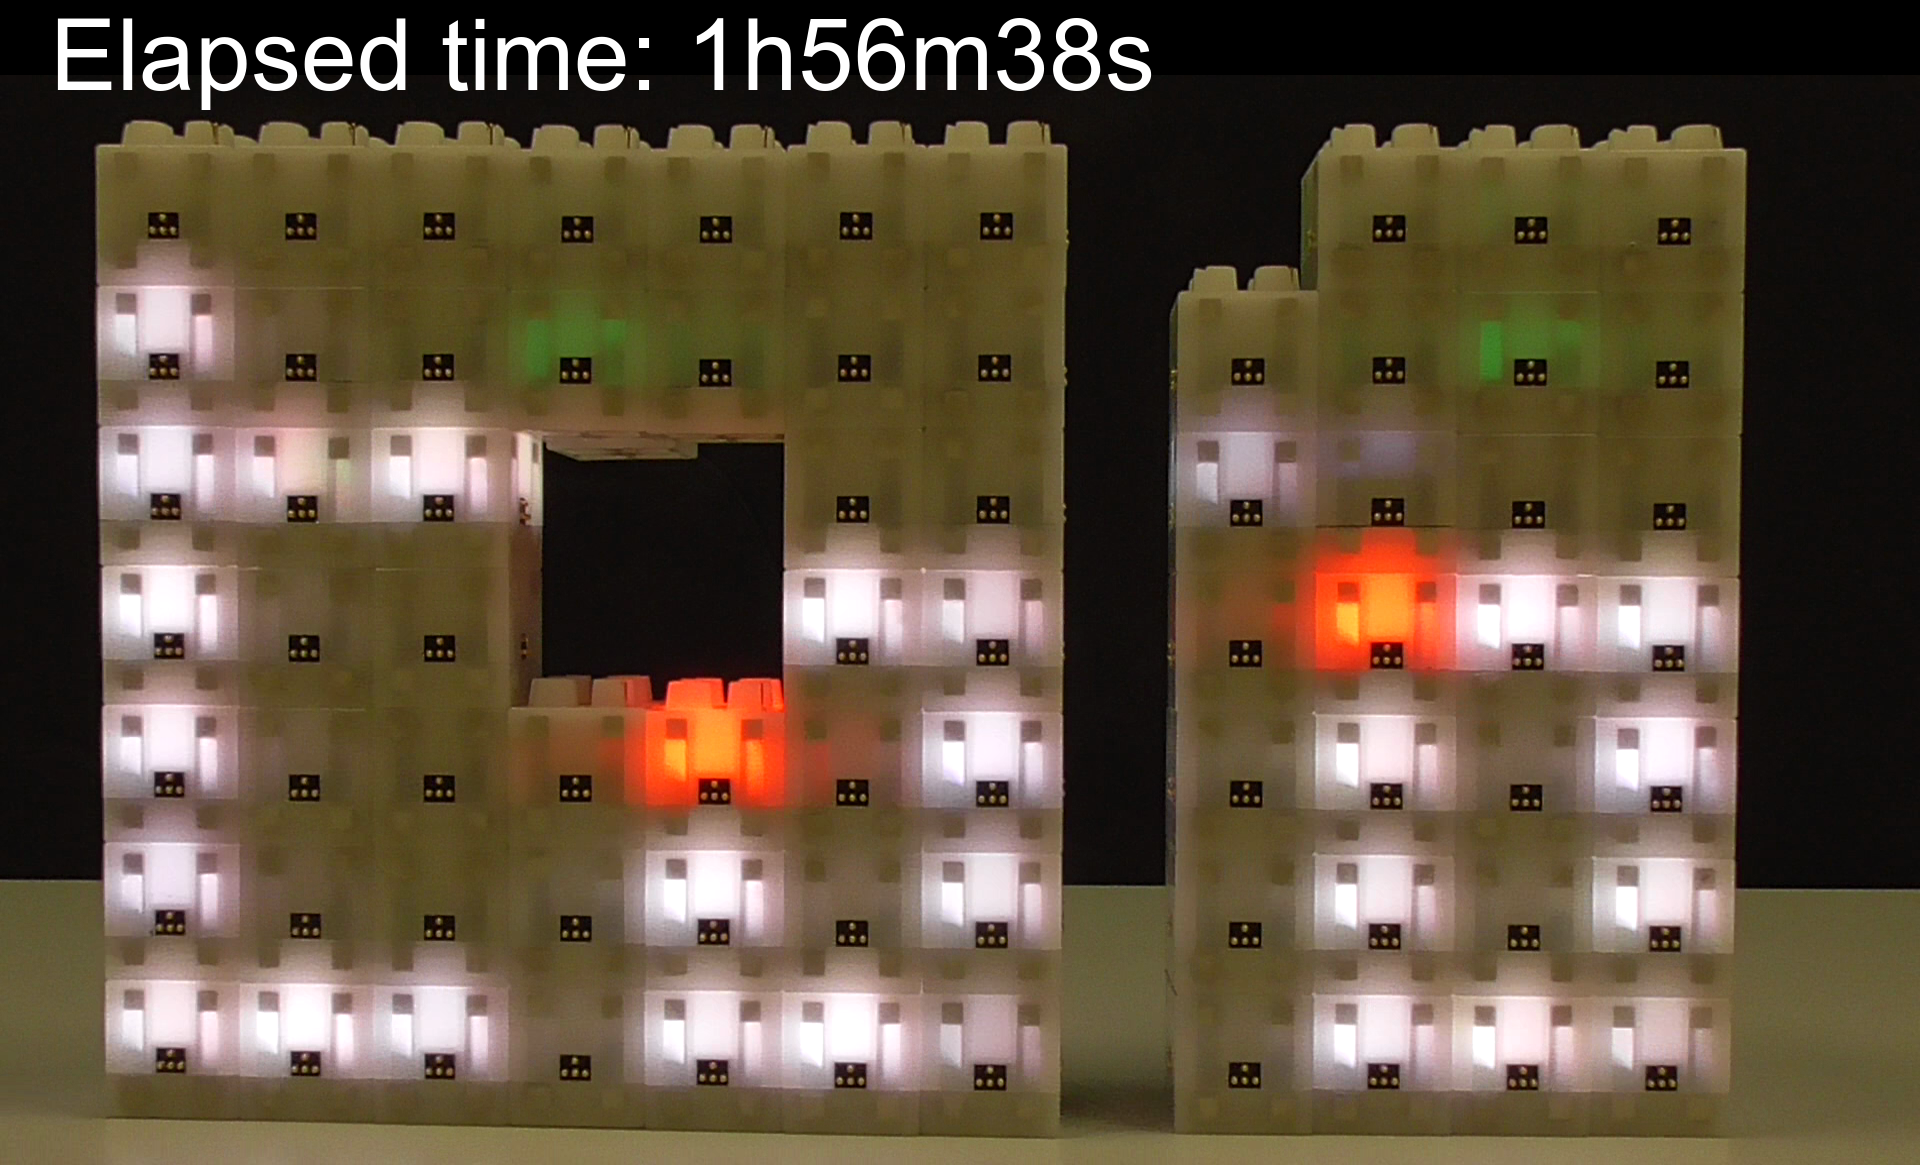
\includegraphics[width=\subFigureWidth]{images/time-synchronization/scroller/sync_1h56m38s} \\
			
			
			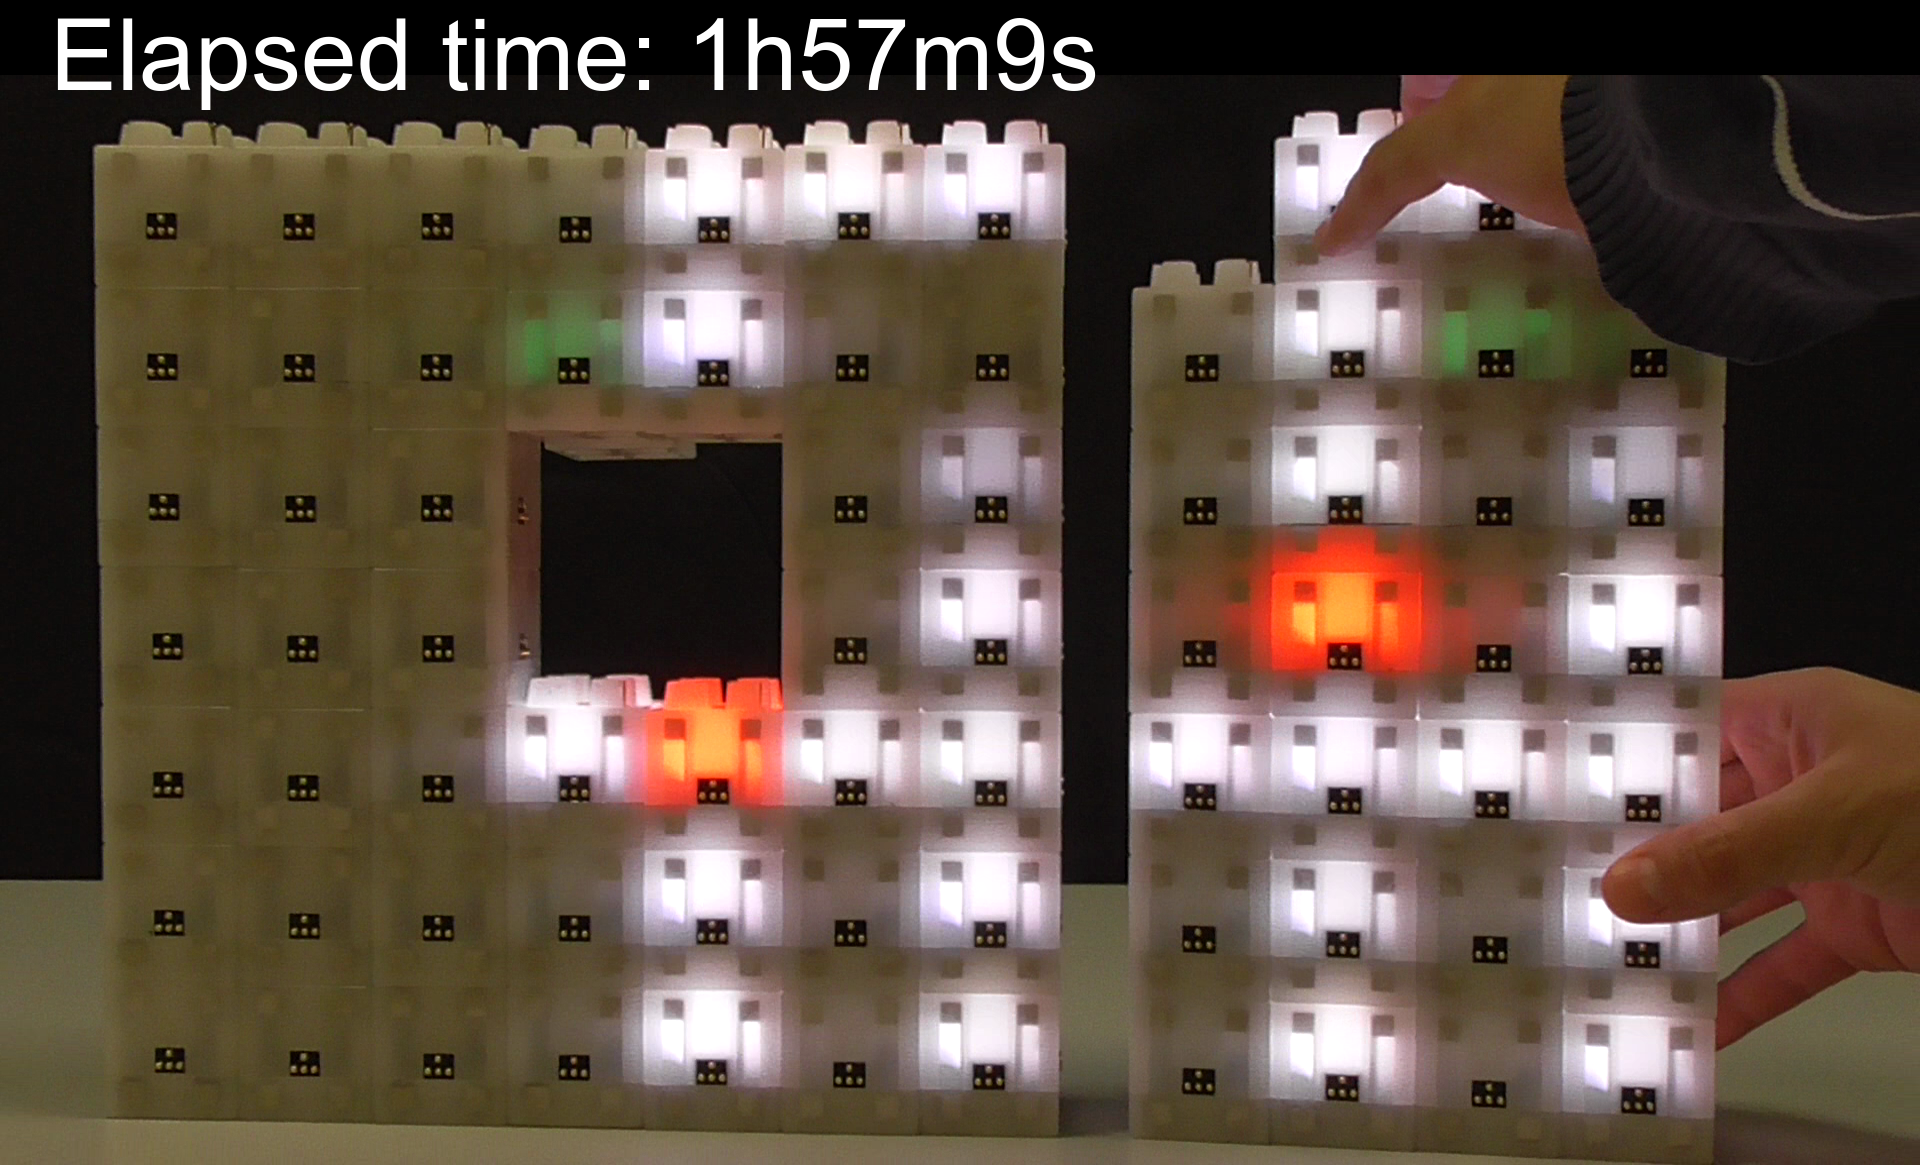
\includegraphics[width=\subFigureWidth]{images/time-synchronization/scroller/sync_1h57m9s} &
			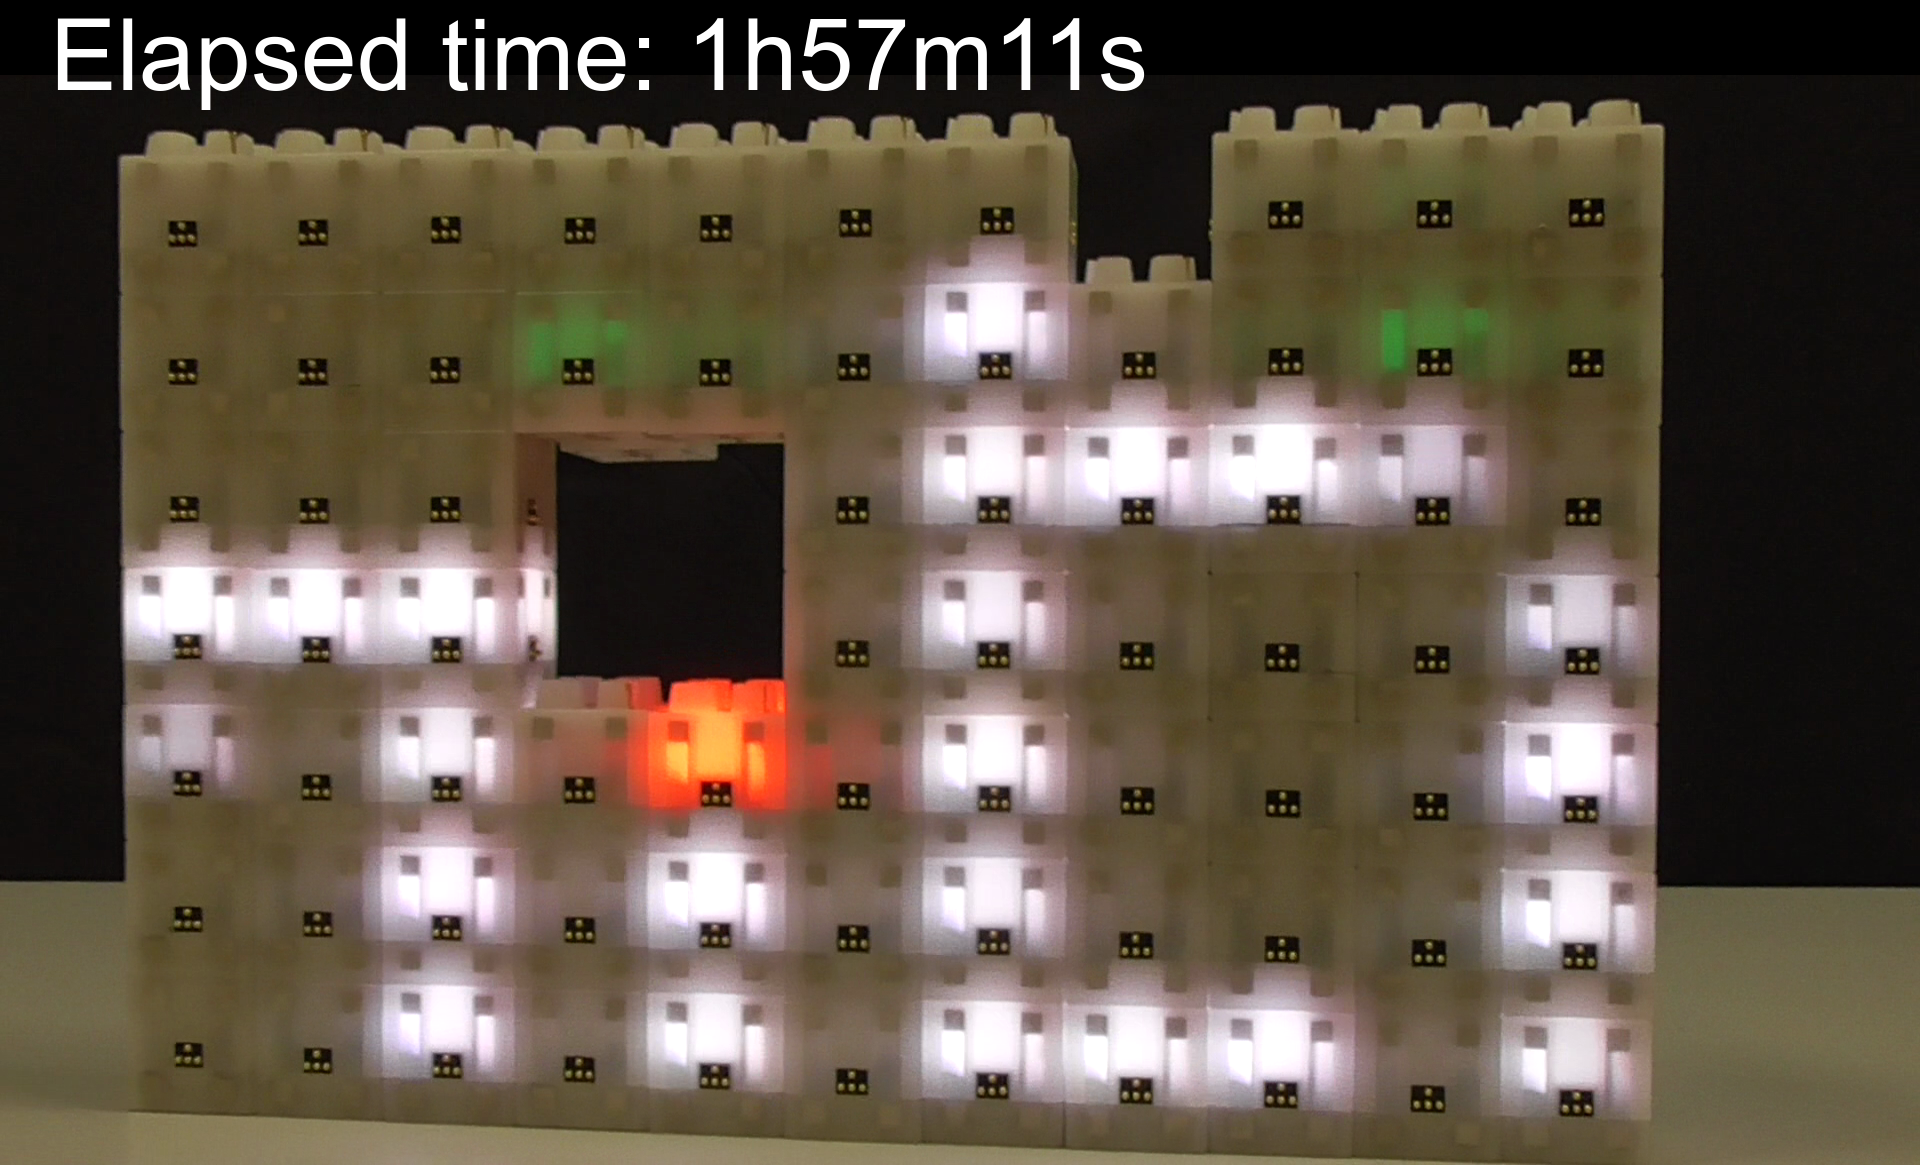
\includegraphics[width=\subFigureWidth]{images/time-synchronization/scroller/sync_1h57m11s}  &
			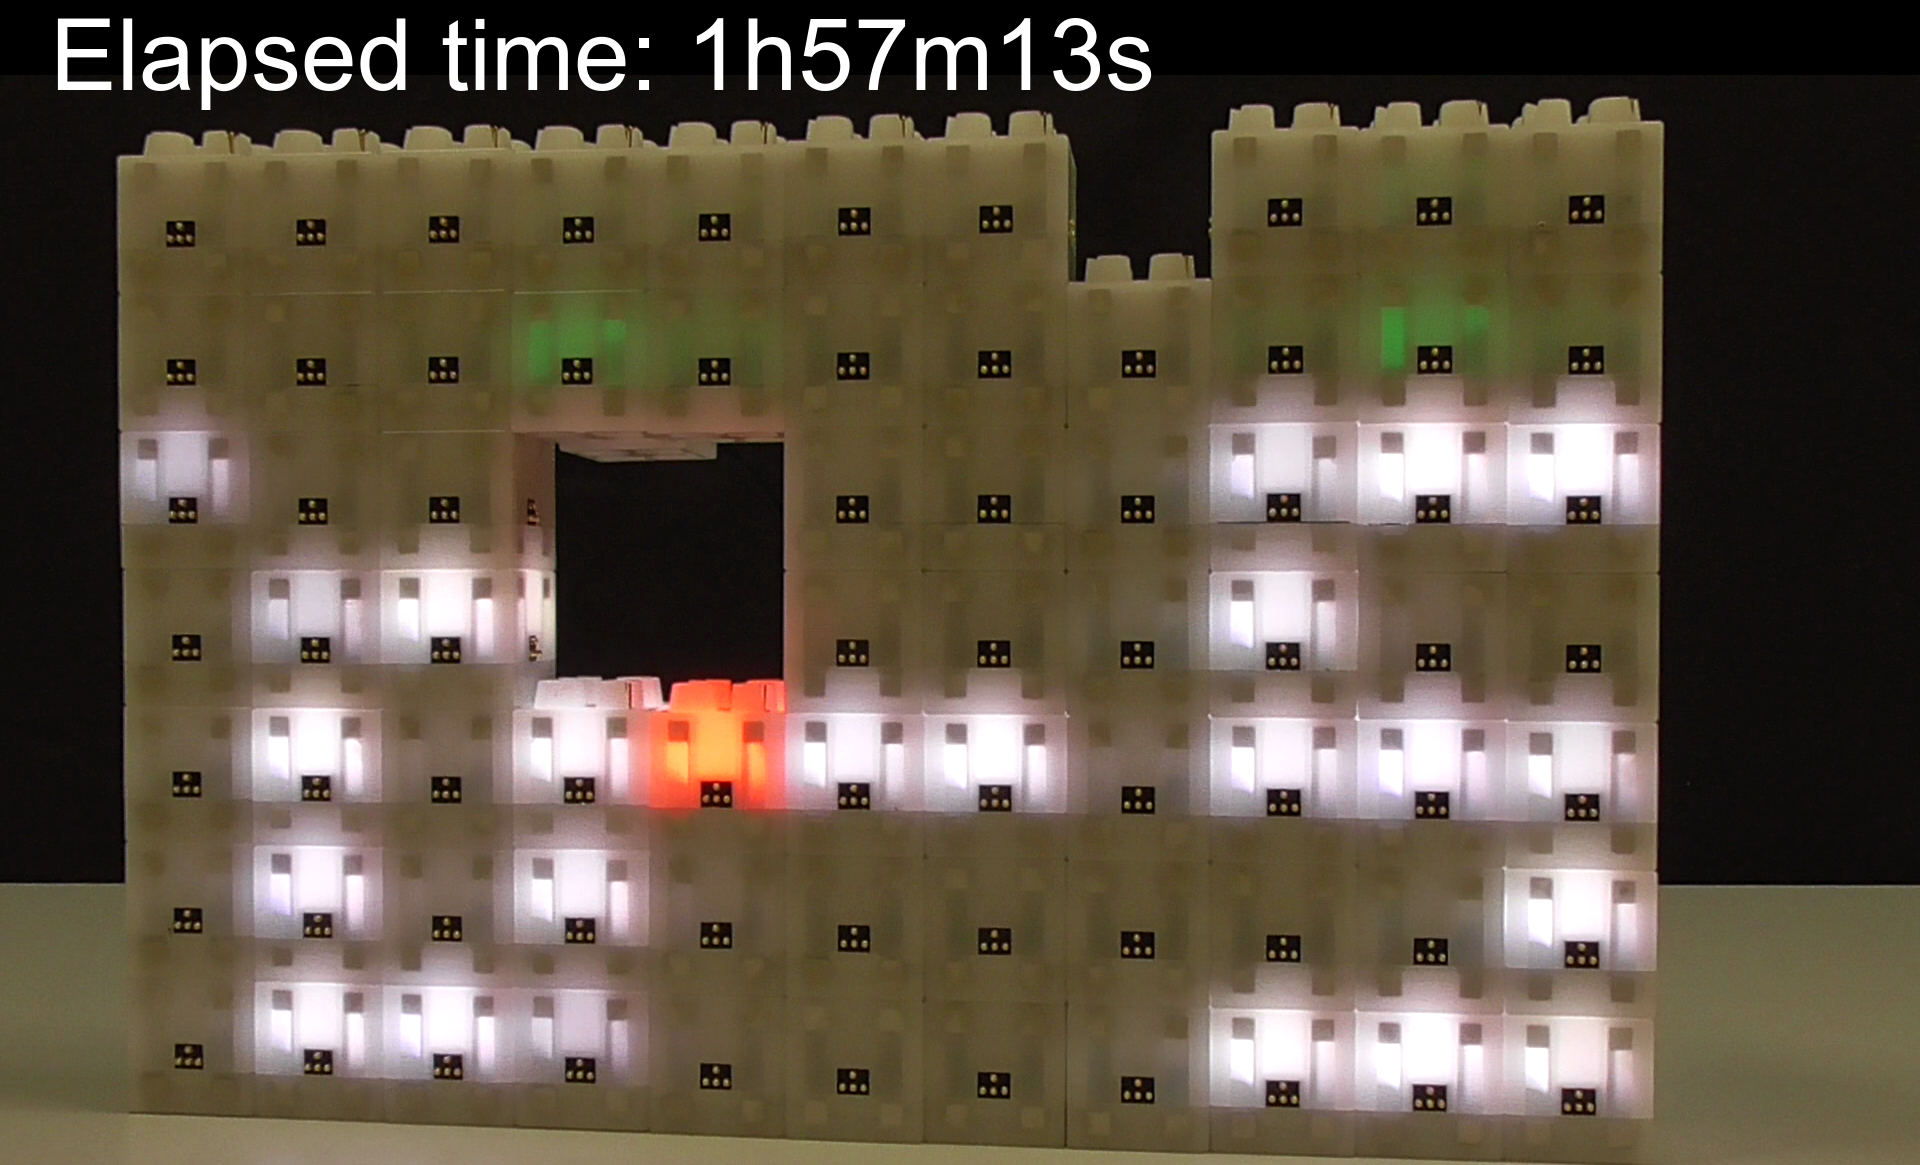
\includegraphics[width=\subFigureWidth]{images/time-synchronization/scroller/sync_1h57m13s}
			
		\end{tabular}	
		\caption{A distributed bitmap scroller made from 72 Blinky Blocks. The system scrolls \inquote{Femto-st} in different colors. The blocks are synchronized using MRTP. The time master stays in red.\label{fig:time-sync:bitmap-scroller}}
	\end{figure}
}

\subsection{Our Implementation}

In our implementation, modules first distributively build a coordinate system. Then, they start to display the text that is shifted one column to the left every 250 milliseconds. From a local point of view, every module stores the global bitmap to display and locally updates its color on a regular basis, based on the module position and on its current clock time, only. The vision persistence is around 40 milliseconds. Hence, when the text is shifted one column to the left, all modules should change their color within 40 milliseconds in order for the color changes to appear synchronized. In our implementation, the system is globally synchronized using MRTP. The time master stays in red.

As shown in Figure~\ref{fig:time-sync:bitmap-scroller}, the bitmap scroller and thus MRTP are robust to system merge and split.

\subsection{Need for Global Time Synchronization}

In order to show that the distributed bitmap scroller requires a global timescale, we sub-sequentially discuss the issues risen by a non-exhaustive list of alternative approaches.

\paragraph{Unsynchronized scroller}

Figure~\ref{fig:time-sync:unsync-bitmap-scroller} shows our implementation of the bitmap scroller running without time synchronization. Because of clock skew, module clocks progressively drift apart from each others causing the modules to light asynchronously and the text being scrolled to become unreadable. Hence, individual color changes need to be synchronized in order to ensure a synchronous scrolling at the global scale.

{
	\newcommand{\subFigureWidth}{0.32\linewidth}
	\begin{figure}[h!]
		\centering			
		\small
		\begin{tabular}{c c c}
			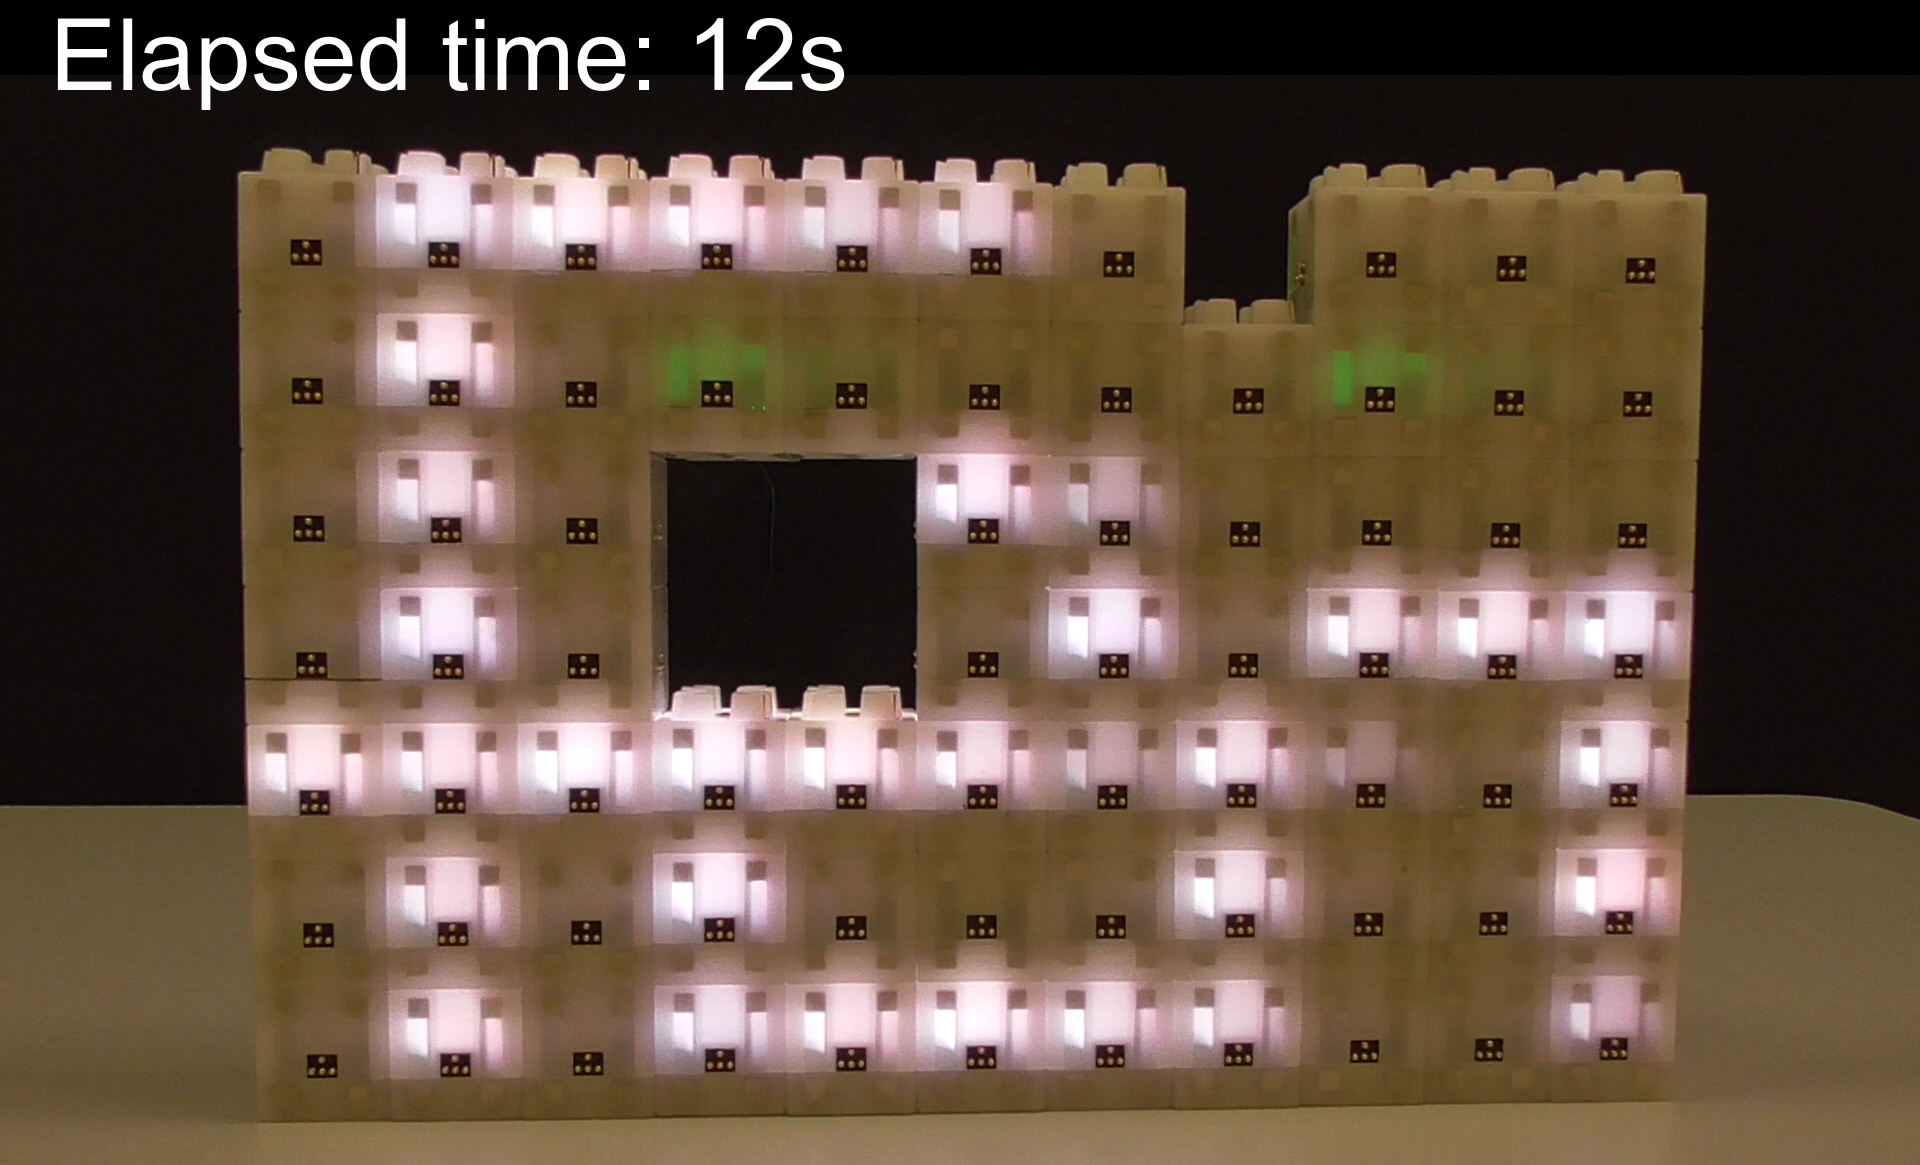
\includegraphics[width=\subFigureWidth]{images/time-synchronization/scroller/unsync_12s}  &
			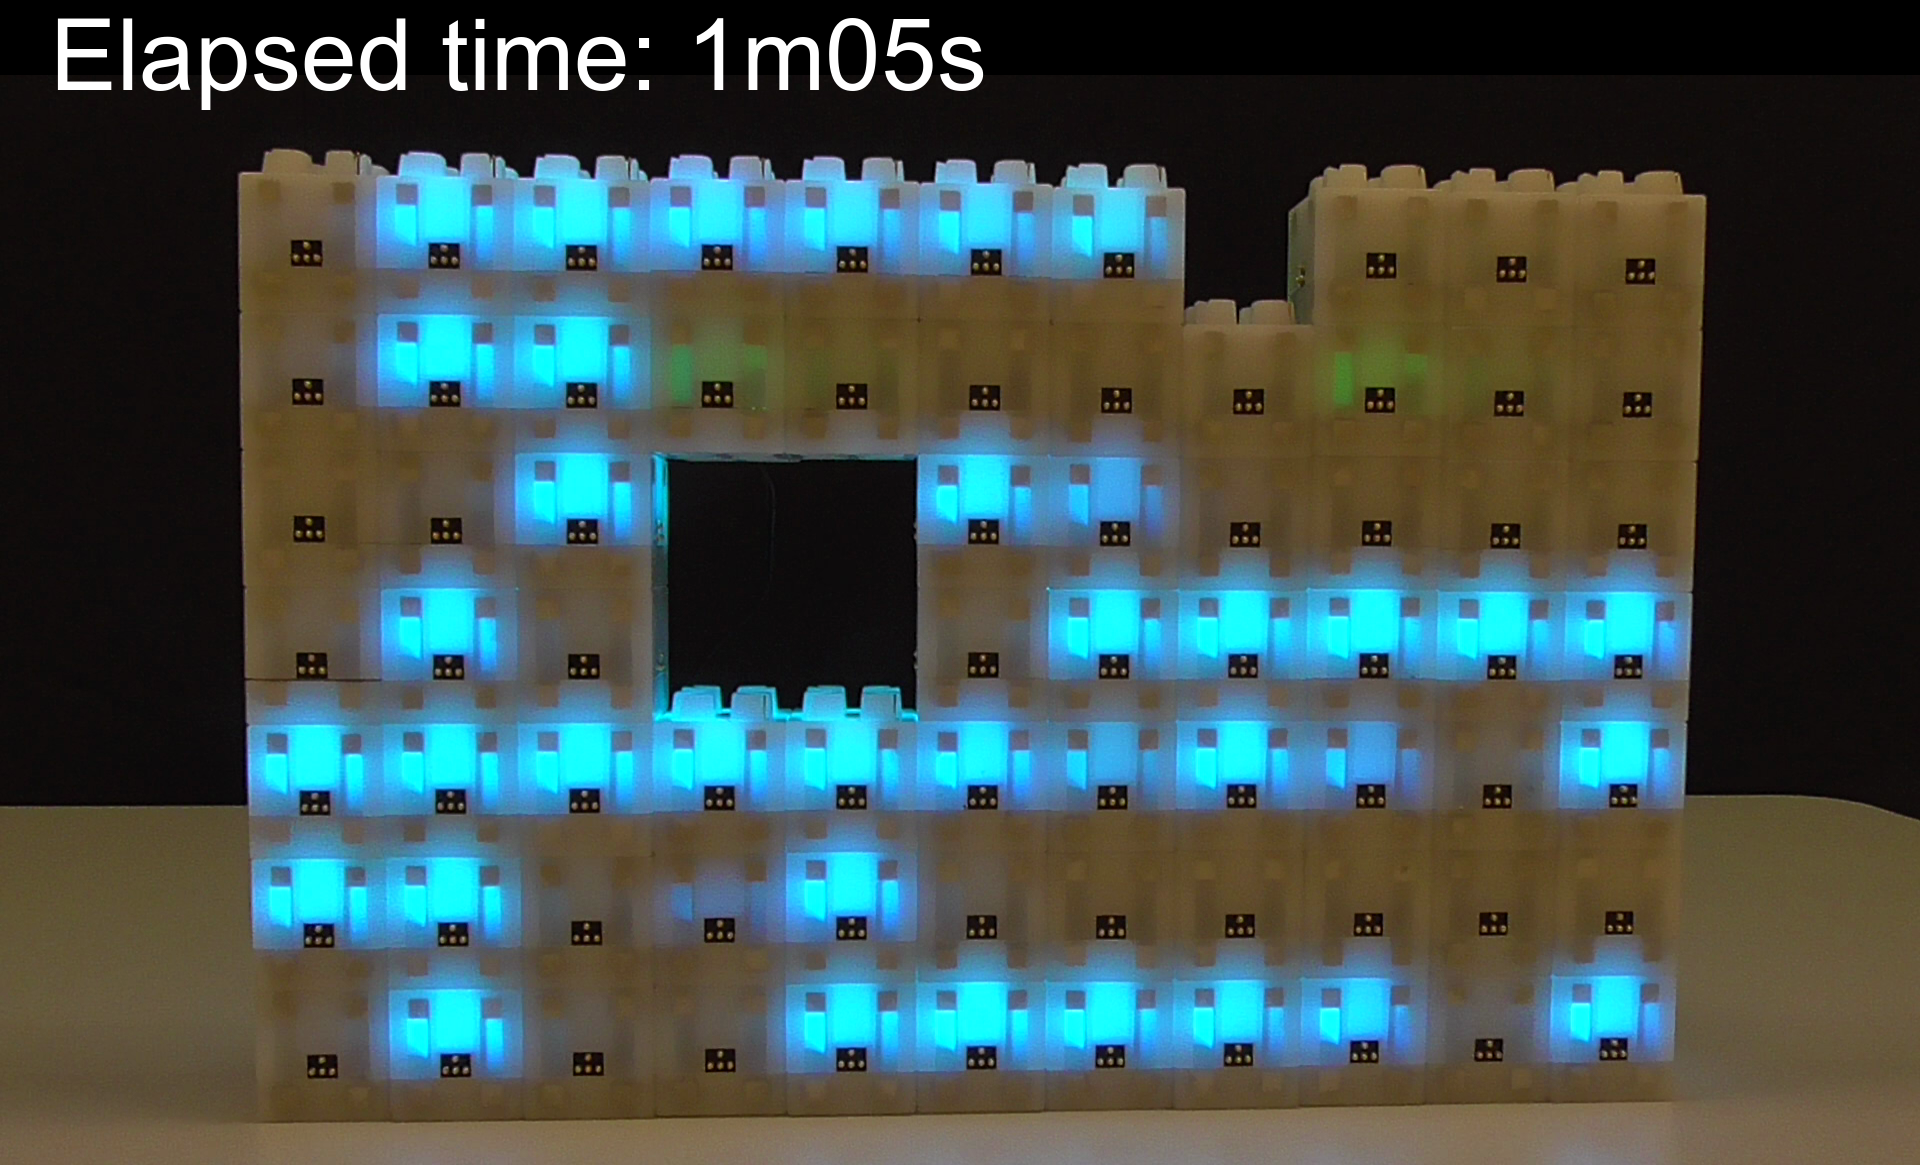
\includegraphics[width=\subFigureWidth]{images/time-synchronization/scroller/unsync_1m05s} & 
			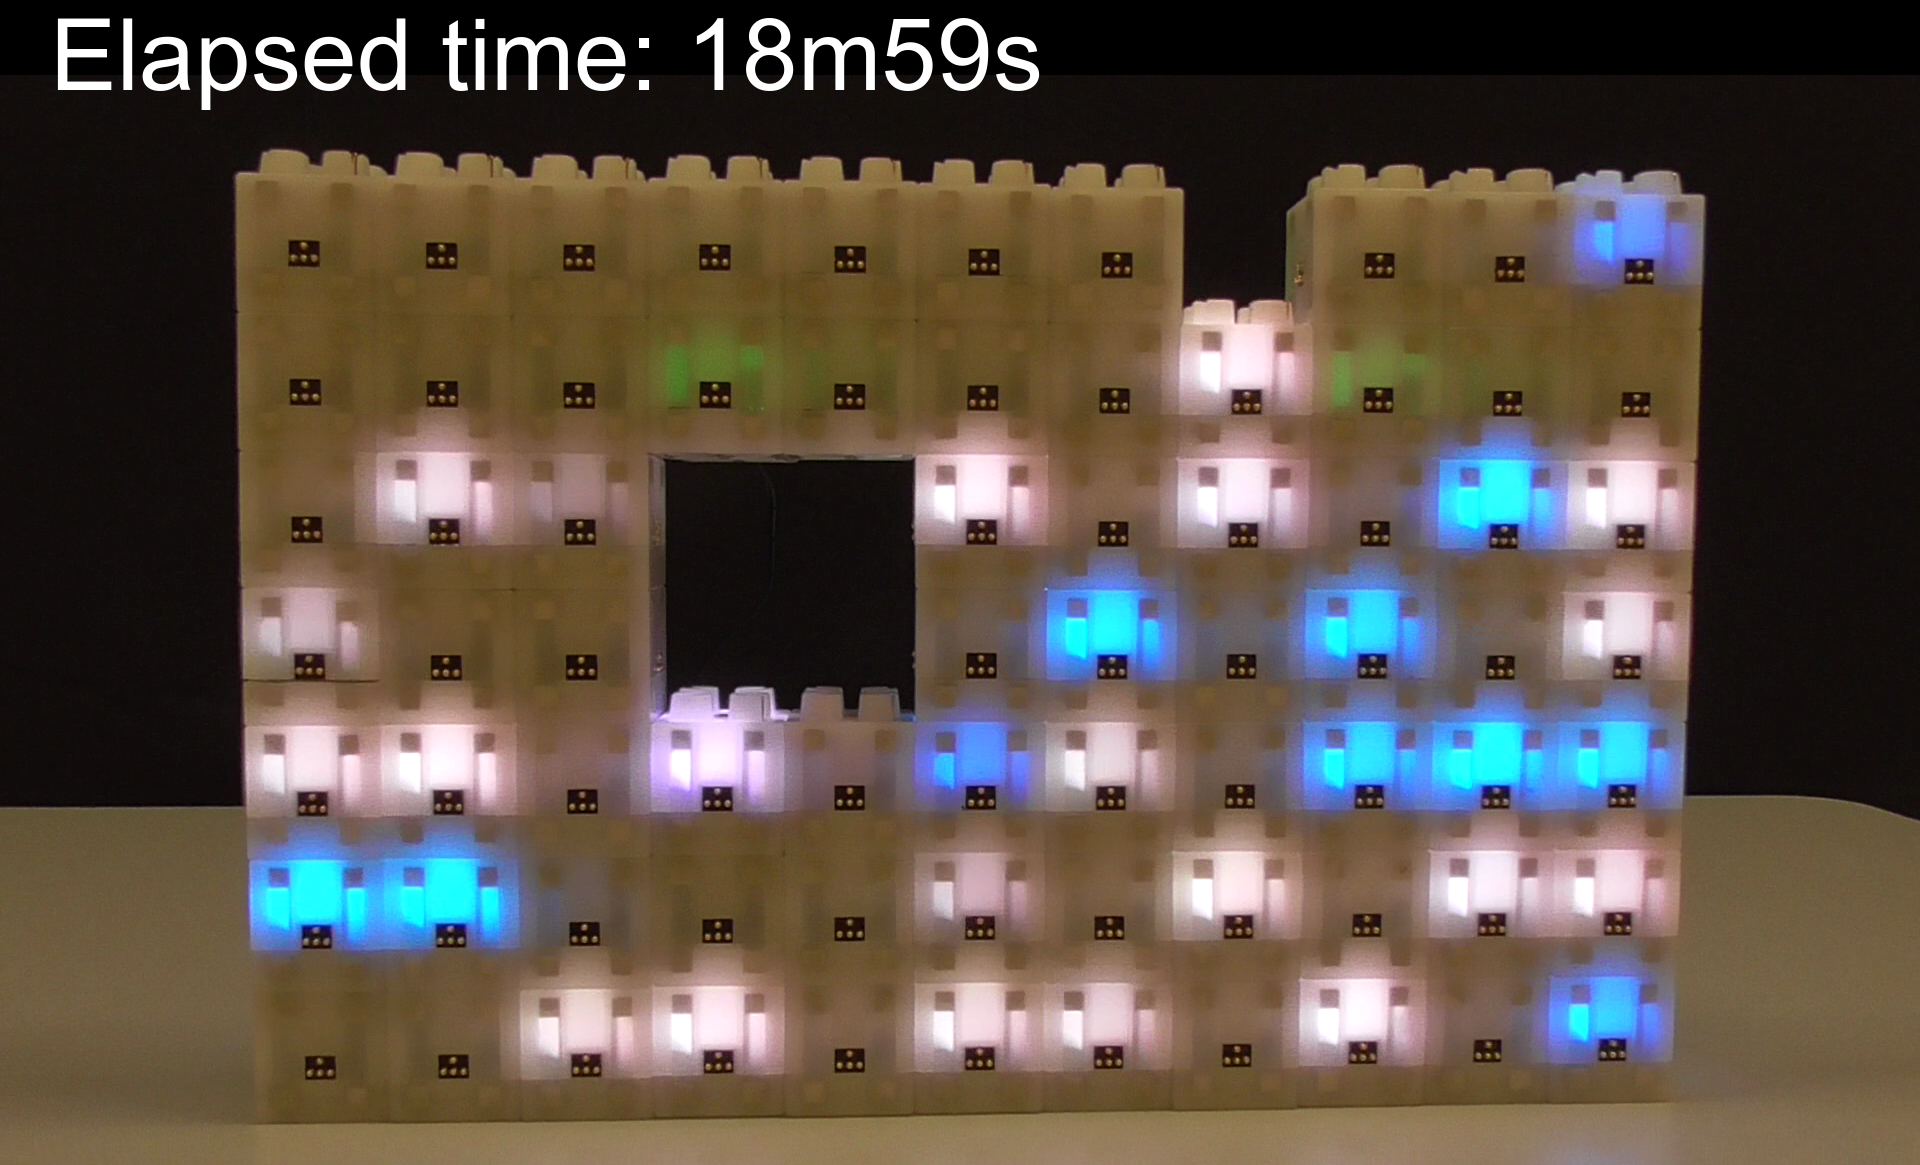
\includegraphics[width=\subFigureWidth]{images/time-synchronization/scroller/unsync_18m59s}
			
		\end{tabular}	
		\caption{Unsynchronized bitmap scroller of 72 Blinky Blocks.\label{fig:time-sync:unsync-bitmap-scroller}}
	\end{figure}
}

\paragraph{Centralized or Distributed Control based on Order Propagation}

A different approach than clock synchronization is to use color change orders to control the system and to dictate the pace of the text shifting.

After having locally observed a delay of 250 ms, a single elected module, or any module, can flood a message to request all the modules to update their color upon reception. However, immediate-term order propagation relies on fast propagation. In our example, a Blinky Block sends a message to a neighboring module on average in 6 milliseconds. If we do not consider message time of residence at nodes, a message needs at least 42 milliseconds to travel over seven hops. Hence, after seven hops, a delay in color changes will be observed and the one-column text shifting will appear unsynchronized.

Color updates can also be scheduled to a future date at which all modules will have received the information. However, it is difficult to predict that time. Indeed, order propagation may be delayed due to the network load for instance. Moreover, it is not possible to precisely schedule a global event too far in the future because of hardware-clock imprecision (skew, noise, etc.).

Moreover, this approach is less robust to message loss than the clock synchronization approach. If an order message is lost, then some modules will not update their color for a step. On the other hand, in our implementation, if an MRTP synchronization message gets lost, all modules will still update their color, but with a slight delay.

\paragraph{Right-to-Left Pixel Propagation}

In this approach, a module holds for 250 milliseconds the current pixel that it has to display. Pixels are propagated from the left to the right using messages to produce column shifts. The right-most module of every row is responsible to start displaying a given pixel. We name these modules the pixel initiators.

An immediate limitation of this approach is that it requires some routing procedure in the presence of holes. Indeed, the left-next module may not be an immediate neighbors. Moreover, this approach less robust to failures than the previous one. Indeed, a pixel gets lost if the message that carries it is lost.

Regarding synchronization, pixel initiators have to be synchronized in order to synchronously start the propagation of the pixels. However, even-though pixel initiators are synchronized, delays in color updates may still be observable. As every module has its own notion of time, pixels will reside at modules for slightly different durations. Hence, pixels will not propagate at the exact same speed in all rows, causing color changes to become more and more unsynchronized with the hop distance.

\paragraph{Limited-scope Time Synchronization}

% Synchronization vs unsynchronization
One may envision to synchronize only neighboring modules together. As shown in the Section~\ref{section:time-sync:large-scale-evaluation}, with this approach, modules are not well synchronized to a global time in large-scale systems. Hence, delays will be observed in the color changes.

Alternatively, one can also envision to synchronize all modules of a same column together. However, because of clock skew, columns will progressively drift apart from each others and color changes will not appear to be all synchronous. Moreover, this approach may be tricky to implement in the presence of holes.

Hence, limited-scope synchronization is not sufficient. In the distributed bitmap scroller, all modules have to synchronously perform an action (i.e., update their color). Hence, all clocks should be synchronized to a global timescale.

\section{State of the Art}

\label{section:time-sync:related-works}

Time synchronization has been extensively studied in various domains. Many algorithms and protocols have been proposed for computer networks such as Cristian's algorithm~\cite{cristian1989proba}, the Berkeley algorithm~\cite{gusella1989accuracy}, the Network Time Protocol (NTP)~\cite{mills1991internet} and the IEEE 1588 Precise Time Protocol (PTP)~\cite{ptp2008}. Time synchronization is also an important topic of interest in \glspl{wsn} where many protocols have been proposed, e.g., Reference Broadcast Synchronization (RBS)~\cite{elson2002fine}, the Timing-sync Protocol for Sensor Networks (TPSN)~\cite{ganeriwal2003timing}, the Flooding Time Synchronization Protocol (FTSP)~\cite{maroti2004flooding}, the Time-Diffusion Synchronization Protocol (TDP)~\cite{su2005time}, the Rapid Time Synchronization (RATS)~\cite{kusy2007spatiotemporal}, the 
PulseSync~\cite{lenzen2009optimal,lenzen2015pulsesync}, the Asynchronous Diffusion algorithm (AD)~\cite{li2006global}, the Gradient Time Synchronization Protocol (GTSP)~\cite{sommer2009gradient}, the Average TimeSynch (ATS) protocol~\cite{schenato2011average} and the Maximum Time Synchronization (MTS)~\cite{he2014time}. Like modular robots, \glspl{wsn} generally form spontaneous peer-to-peer networks of resource-constrained devices. To the best of our knowledge, time synchronization has not attracted any attention in the modular robotic community. Methods to provide a global metronome-like signal in modular robots have been proposed in~\cite{kokaji1996clock, baca2010synchronizing}. However, these mechanisms synchronize clock phase or/and frequency, but not actual clock time. Moreover,~\cite{kokaji1996clock} is purely theoretical, the authors consider ideal clocks running at the same exact frequency and do not provide any performance evaluation. In~\cite{Stoy03,stoy2002make,stoy2002global}, the authors propose the role-based distributed control algorithm for modular robotic systems. It enables to coordinate module actions in order to produce a global behavior. In this method, a periodic logical signal is established in the system using message passing (e.g., a sine wave signal to produce a caterpillar-like locomotion in a chain of modules). However, this control method does not establish a global timescale and ignores communication delays.

\subsection{Architecture : from Master/Slave to fully Distributed Protocols}

Existing time synchronization protocols differ by the network architecture they adopt. NTP, PTP, TPSN, FTSP, PuleSync, RBS and TDP adopt a master/slave approach. In a master/slave approach, one or more masters are in charge of synchronizing slave nodes. In NTP, PTP, TPSN, FTSP, PuleSync and TDP, slave node clocks are adjusted to a reference time held by the time master(s). The reference time can be the Coordinated Universal Time or the master local clock. In the Berkeley algorithm, slave node clocks are adjusted to an aggregated value of some or all the system clock values. These approaches aim at performing global synchronization, i.e., keeping all nodes synchronized together. These protocols provide a satisfactory synchronization precision between arbitrary nodes but may poorly synchronize neighboring nodes. This is due to the fact that two neighboring nodes can be synchronized by messages that have traveled on long and almost independent paths, causing the error accumulated at every hop to be propagated differently.

In contrast, AD, ATS, GTSP and MTS are fully distributed. In these protocols, nodes exchange timing information with all their one-hop neighbors on a regular basis. In AD, every node frequently adjusts its clock to the average value of its neighbors' clock. ATS and GTSP use a similar consensus-based averaging technique. These average-based approaches primarily aim at achieving local synchronization, i.e., keeping neighboring nodes synchronized together, allowing nodes to have a larger pairwise synchronization error with nodes that are faraway. MTS and its variants proposed in~\cite{he2014time,he2014study} use extremum-value-based consensus to achieve faster convergence. In general, fully distributed methods are naturally fault-tolerant and robust to node mobility. However, they can lead to a long convergence time and to a high message complexity, especially in point-to-point networks without broadcast support. Indeed, in systems without local or global shared broadcast medium, a node has to send individual messages to all neighbors in order to broadcast messages.

\subsection{Infrastructure of Master/Slave Protocols}
\label{section:synchronization:related-work:infrastructure}

\newcommand{\InfrastructureLess}{infrastructure\hyp less}

Master/slave time synchronization protocols differ by the infrastructure they use. Protocols can use tree-like structures, cluster-based structures or be infrastructure-less.

\paragraph{Tree-like Structures}

NTP, PTP and TPSN use tree-like hierarchical structures rooted at the time master(s) to spread timing information. Logical neighbors in the tree(s) can be neighbors in the physical network as in TPSN, or potentially distant as in NTP. The latter case may require multi-hop communications that rely on the existence of an underlying routing service. In our case, we assume no routing service. In TPSN, nodes are recursively synchronized hop-by-hop along the edges of the synchronization tree starting from the time master. Hence, during each synchronization phase, the current global time gets quickly disseminated through the entire network. In addition to providing a relatively quick synchronization convergence, this reduces the impact of clock inaccuracies (due to noise, skew variations, time-increasing errors in the local estimation of the global time) on the synchronization process. 

\paragraph{Clustering based on Broadcast Domains} In RBS, nodes maintain relative timescales of their neighborhood using reference pulses broadcast by some master nodes. In multi-hop networks, nodes can be grouped into overlapping clusters based on broadcast domains and border nodes act as gateways to translate clock values. 

\paragraph{Infrastructure-less Approaches}

In contrast, FTSP, RATS and PulseSync are infrastructure-less. They provide robustness to network topology changes and to link failures using either periodic local broadcasts or periodic network-wide floodings. In FTSP, the time master and the synchronized nodes periodically broadcast their estimation of the current global time to all their neighbors, in an asynchronous way. Synchronization waves propagate with a limited speed through the network. Indeed, after having received a new synchronization message, a node has to wait until the expiration of its broadcast period to transmit the information to its neighbors. As a consequence, the time-increasing estimation error of the global time is amplified at every hop and FTSP exhibits a synchronization error that grows exponentially with the size of the network~\cite{lenzen2009optimal}. Hence, optimal synchronization requires fast network flooding~\cite{lenzen2009optimal}. RATS and PulseSync employ rapid network-wide floodings using recursive broadcasts to quickly disseminate the global time through the network. The time master periodically launches synchronization waves using broadcasts. Slave modules re-broadcast new synchronization messages shortly after reception. In~\cite{ferrari2011efficient}, the authors propose a sophisticated mechanism to provide fast network flooding in IEEE 802.15.4 \glspl{wsn} and thus accurate time synchronization. In reliable and fairly static point-to-point networks without broadcast support, recursive synchronizations using a tree-like structure are more communication-efficient than network-wide flooding.

\subsection{Communication Delay Compensation Methods}
\label{section:time-sync:communication-delay-comp-methods}

Time synchronization protocols also differ by the methods they use to compensate for communication delays. The method to be applied depends on the target platform and more precisely on the communication mechanism and the precision with which time can be measured. This choice directly impacts the precision of the synchronization protocol. Existing methods can be divided into three categories: approaches based on the round-trip time, methods based on byte-level timestamping and approaches based on reference broadcasts.

\paragraph{Round-Trip Time based Methods}

Cristian's algorithm, the Berkeley algorithm, NTP, PTP, TPSN and TDP measure half the round-trip time to estimate one-way communication delays. Cristian's algorithm and NTP perform end-to-end synchronization on possibly multi-hop paths. They use statistical analysis to mitigate variations in delays due to retransmission(s), queueing, route selection, etc. These methods are expensive in communications and in computations. PTP and TPSN propose to perform per-hop synchronization with low-level timestamping to prevent unpredictable delays induced at the different layers of the network stack from affecting delay measurements. PTP can use timestamps recorded at the physical layer to achieve high accuracy if dedicated hardware is available. In TPSN, a node exchanges a single bidirectional message timestamped at the boundary of the data-link layer to synchronize itself to another node and compensates for communication delays using half the round-trip time. We call this method RTT (for Round-Trip Time). Round-trip time methods assume symmetrical nominal delays and usually neglect the effect of clock skew during the round trip. In~\cite{syed2006time}, Syed et al. study time synchronization in underwater acoustic sensor networks where propagation times of several hundred milliseconds are observed. They propose to use skew-compensated two-way message exchanges in these systems.

%https://www.ietf.org/rfc/rfc5905.txt
% NTPv4
%If the NTP has access to the physical layer, then the timestamps are
%associated with the beginning of the symbol after the start of frame.
%Otherwise, implementations should attempt to associate the timestamp
%to the earliest accessible point in the frame.

\paragraph{Byte-level Timestamp based Methods}

FTSP, PulseSync and the practical implementations of both ATS~\cite{schenato2011average} and MTS~\cite{he2014study} use byte-level time\hyph stamping, which requires an intimate access to the data-link layer.

In the last two methods, nodes exchange a single unidirectional message timestamped just before the transmission of the first byte (i.e., the Frame Delimiter byte) and upon reception of this byte. The time elapsed between the transmission and the reception of the frame delimiter byte is neglected and ATS~/~MTS consider that the two timestamps refer to the same real time. We call this method FD (for Frame Delimiter). This method neglects the interrupt handling time, the frame delimiter byte transmission~/~reception, the propagation time and the time required for the detection of the frame delimiter byte. Although FD works well in low-latency networks, the neglected time can be important in higher-latency systems. For instance, our target system uses 38.4 kbit/s connections while \glspl{wsn} that use IEEE 802.11b communications have a maximal bitrate of 11 Mbit/s.  At 38.4 kbit/s, a byte is transmitted in roughly 208 $\mu s$, while at 11 Mbit/s a byte is sent in less than 1 $\mu s$.

FTSP goes one step further in order to eliminate most of the sources of delays in message transmission (except for the propagation time). FTSP synchronizes neighbors using a single message broadcast with statistical operations on timestamps captured at the byte boundary during interrupts at the data-link layer. The latest version of PulseSync~\cite{lenzen2015pulsesync} is based on an enhanced version of the FD method. The authors use the slotted programming approach~\cite{flury2010slotted} to minimize the interrupt latency and use a static value measured experimentally during a calibration phase to compensate for the time between the insertion of the timestamp, just before transmitting the frame delimiter byte, and its detection upon reception. However, the method proposed in FTSP and PulseSync cannot be applied directly to our target system. Indeed, we assume low-resolution clocks, typically in the order of the millisecond, that cannot efficiently capture phenomena at the byte transmission level which occurs on the microsecond scale.

\paragraph{Reference Broadcast}
In RBS, some reference nodes periodically broadcast reference messages. Neglecting propagation delays, receiving nodes use the data-link reception times as reference points to compare their clock values all together. This requires a shared broadcast medium and it is not usable in point-to-point networks.

\paragraph{Discussion}
We argue that the method of compensating for communication delays has to be selected as a function of the target system. If we assume a predictable transfer time between neighbor modules, we propose to perform per-hop synchronization using a single unidirectional message timestamped at the data-link layer and predictive communication delay compensation (see Section~\ref{section:time-sync:pred-method}). We call this method PRED (for Predictive). We show in the evaluation section~\ref{section:time-sync:delay-comp-method} that, in our target system, PRED is on average more precise than the other two methods that can be applied to our target system, namely FD and RTT. Note that this is mainly due to the fact that the average transfer delay of a frame is almost a round number (on the millisecond scale) in this system.

\subsection{Clock Model: from Clock Offset Adjustment only to Clock Skew Compensation}

% http://stackoverflow.com/questions/19352740/how-does-ntp-clock-discipline-work

Furthermore, time synchronization protocols differ in the clock model they use. In some protocols, e.g., AD and TPSN, nodes perform clock offset adjustment only and do not take into account clock skew. Compensation for clock skew enables modules to be synchronized less frequently without degrading the synchronization precision. 

NTP uses phase-locked loops and/or frequency-locked loops. In~\cite{kim2012tracking}, the authors use a Kalman filter to track clock offset and skew with low-precision oscillators and time-varying skew. Indeed, in the presence of ambient environment variations (e.g., temperature variations), the clock skew may vary over time. 

ATS, Belief Propagation (BP)~\cite{etzlinger2014cooperative}, GTSP, Mean Field (MF)~\cite{etzlinger2014cooperative}, MTS, FTSP, RBS, PulseSync, RATS and~\cite{noh2007novel,leng2010clock} propose to model clock using a linear model computed from recent observations, assuming that oscillators have high short-term stability. Indeed, if we assume that environment changes do not happen or happen gradually, the clock skew will change smoothly. RBS, FTSP, PulseSync and RATS use least-square linear regression on a recent window of observations. ATS and GTSP use an averaging technique to estimate the clock skew based on the previous synchronization point. In~\cite{noh2007novel,leng2010clock}, the authors propose to enhance TPSN by using a linear model and maximum likelihood estimators. BP and MF derive maximum a posteriori estimators of the clock parameters using belief propagation and mean field on factor graphs, respectively. Different methods for clock skew compensation including linear regression, exponential averaging and phase-locked loops have been evaluated in~\cite{amundson2008time}. Although results are nearly identical, experiments suggest that linear regression leads to slightly more precision.

Note that, in addition to compensating for clock skew, these aggregating techniques also tend to reduce the impact of the measurement errors due to the resolution of the timestamps.

\subsection{Time Master Election}
\label{section:time-sync:time-master}

Master/slave time synchronization protocols also differ by the mechanisms they employ to select the time master. In NTP and RATS, time masters are pre-configured. In our case, it is more flexible if the system itself elects its time master. In PTP and TDP, elections are based on the quality of the clocks. In addition, TDP periodically re-elects time masters to balance the load. FTSP and PulseSync implicitly elect the minimum-identifier node as the time master during the synchronization phases. 

In our case, we consider systems where all modules are identical and equipped with the same hardware clocks. Although these clocks differ slightly in their accuracy and stability, we consider that with a careful selection of the hardware, the impact of cumulative errors in network delay estimations will be predominant in large-diameter systems. A random error is experienced at each hop. Let us assume that these per-hop errors are independent and identically distributed with a mean of $\lambda$ and a standard deviation of $\sigma$. The Central Limit theorem states that the error accumulated over $k$ hops follows a normal distribution with a mean of $\lambda k$ and a standard deviation of $\delta\sqrt{k}$. Experimental results presented in Section~\ref{section:time-sync:delay-comp-method} confirm this trend. Hence, we propose to elect a central module as the time master.

\subsection{Summary}

{
	\newcommand{\lenMinusOne}{0.11\linewidth}
	\newcommand{\lenZero}{0.09\linewidth}
	\newcommand{\lenOneFour}{0.15\linewidth}
	\newcommand{\lenOneThree}{0.12\linewidth}
	\newcommand{\lenTwo}{0.15\linewidth}
	\newcommand{\lenTwoOne}{0.14\linewidth}
	\newcommand{\lenThree}{0.17\linewidth}
	\newcommand{\lenFour}{0.24\linewidth}
	
	\linespread{1}\selectfont
	
	\begin{table}[h!]
		%\footnotesize
		\scriptsize
		%\tiny
		%\tiny
		\begin{center}
			\resizebox{\textwidth}{!}{\begin{tabular} {|C{\lenOneThree}|C{\lenZero}|C{\lenTwoOne}|C{\lenMinusOne}|C{\lenFour}|C{\lenOneFour}|}
					\hline
					Name &  Domain & Architecture & Infrastructure & Synchronization Technique & Clock Skew Compensation\\
					\hline
					NTP~\cite{mills1991internet} & Computer Networks & Master/Slave Master(s): pre-configured & Tree & (Multi-hop) round-trip messages with frame-level timestamps and statistics & Phase-locked and/or frequency-locked loops \\
					\hline
					PTP~\cite{ptp2008} & Computer Networks & Master/Slave Master: clock quality based election & Tree & Round-trip messages with low-level (data-link to physical layer) timestamps and per-hop delay compensation & \\
					\hline
					TPSN~\cite{ganeriwal2003timing} & Sensor Networks & Master/Slave & Tree & Recursive per-hop synchronization. Round-trip messages with frame-level timestamps  & / \\
					\hline
					%~\cite{ganeriwal2003timing} 
					TPSN + MLE~\cite{leng2010clock} & Sensor Networks & Master/Slave & Tree & Recursive per-hop synchronization. Round-trip messages with frame-level timestamps and statistics & Linear model with maximum likelihood estimators \\
					\hline
					TDP~\cite{su2005time} & Sensor Networks & Masters/Slave multiple changing masters: clock quality based election & / & Recursive per-hop synchronization. Bidirectional round-trip messages with statistics & / \\
					\hline
					RBS~\cite{elson2002fine} & Sensor Networks & Master/Slave & Broadcast-domain based clustering  & Reference broadcast  & Linear model with least-square linear regression \\
					\hline
					%CLTS~\cite{van2003lightweight} & Sensor Networks & Master/slave & Minimum-depth tree & Pairwise: per-hop round-trip with frame-level timestamps & / \\
					%\hline
					%Tiny-Sync and Mini-Sync~\cite{sichitiu2003simple} & Sensor Networks & ? & Tree & & Linear model with linear programming problem solving\\
					%\hline			
					FTSP~\cite{maroti2004flooding} & Sensor Networks & Master/Slave Master: id-based implicit election& / & Periodic asynchronous broadcasts. Unidirectional broadcast with byte-level timestamps and statistics & Linear model with least-square linear regression \\
					\hline
					RATS~\cite{kusy2007spatiotemporal} & Sensor Networks & Master/Slave Master: pre-configured & / &  Recursive per-hop synchronization. Unidirectional broadcast with byte-level timestamps and statistics & Linear model with least-square regression\\
					\hline				
					Pulse-Sync~\cite{lenzen2009optimal,lenzen2015pulsesync} & Sensor Networks & Master/Slave Master: id-based implicit election& / & Recursive per-hop synchronization. Unidirectional broadcast with byte-level timestamps and statistics & Linear model with least-square linear regression \\
					\hline
					%FCSA~\cite{yildirim2014time} & Sensor Networks & Master/Slave Master: pre-configured & / & & Linear model with least-square regression\\
					%\hline
					%HRTS~\cite{dai2004tsync} & Sensor Networks & Master/Slave & Broadcast-domain based clustering & Broadcast: overheard round-trip with frame-level timestamps  & / \\
					%\hline
					AD~\cite{li2006global} & Sensor Networks & Fully distributed & / & Average-based consensus & / \\
					\hline			
					GTSP~\cite{sommer2009gradient} & Sensor Networks & Fully distributed & / & Average-based consensus. Unidirectional broadcast with byte-level timestamps and statistics & Linear model with an averaging technique\\
					\hline
					ATS~\cite{schenato2011average} & Sensor Networks & Fully distributed & / & Average-based consensus. Unidirectional broadcast with byte-level timestamps & Linear model with an averaging technique\\
					\hline
					MTS and its variants~\cite{he2014time,he2014study} & Sensor Networks & Fully distributed & / & Extremum-value based consensus. Unidirectional broadcast with byte-level timestamps & Linear model with possibly an averaging technique\\
					\hline
					%ADMM~\cite{zennaro2011fast} & Sensor Networks & Fully distributed & / & alternating direction of multiplier method based consensus & Linear model\\
					%\hline
					%LCS~\cite{solis2006new} & Sensor Networks & & / & & Linear model with recursive least-square regression\\
					%\hline
					BP and MF~\cite{etzlinger2014cooperative} & Sensor Networks & Master/Slave or fully distributed & / & Belief propagation and mean field. Single-hop bidirectional messages with frame-level timestamps & Linear model with maximum a posteriori estimators\\
					\hline
			\end{tabular}}
		\end{center}
		
		\begin{center}
			
			\resizebox{\textwidth}{!}{\begin{tabular}{|C{\lenOneThree}|C{\lenZero}|C{\lenTwoOne}|C{\lenMinusOne}|C{\lenFour}|C{\lenOneFour}|}
					\hline
					Our Contribution: MRTP  & Modular Robotic & Master/Slave Master: centrality-based election & Tree & Recursive per-hop synchronization. Selection of the most suited communication delay compensation method for the target system &  Linear model with least-square linear regression\\
					\hline
			\end{tabular}}
		\end{center}
		\vspace{-0.5cm}
		\caption{Summary of the state of the art on time synchronization.}
		\vspace{-0.75cm}
		\label{table:time-sync:related-work-summary}
	\end{table}
}


Table~\ref{table:time-sync:related-work-summary} summarizes the related work. Existing protocols contain interesting ideas but fail to efficiently adapt to homogeneous modular robot systems where modules use low-bitrate neighbor-to-neighbor communications, hardware clocks have low precision and the network diameter can be large.  In the absence of a (locally) shared communication medium, infrastructure-less approaches are too expensive in terms of communication in compact systems compared to tree-based approaches. The method to compensate for network delays has to be carefully selected in function of the target platform. Furthermore, criteria considered for time master election are not adapted to modular robots running under our assumptions. Node centrality can be considered for the election in order to increase the overall synchronization precision.

\section{System Model and Assumptions}
\label{section:time-sync:model}

In this chapter, we consider modular reconfigurable robots that form asynchronous non-anonymous point-to-point connected networks in which modules use neighbor-to-neighbor communications. We assume that every module has a unique identifier and maintains a consistent list of its neighbors. Furthermore, our protocol is intended to synchronize fairly stable systems where changes in the network topology, due for instance to module mobility, or potential module or link failures, are infrequent. A modular robot can be modeled by an undirected and unweighted graph of interconnected entities $G = (V,E)$, with $V$ the set of vertices representing the modules, E the set of edges representing the connections, $|V|=n$, the number of vertices and $|E|= m$, the number of edges. We use the general graph theory concepts such as the distance between two nodes and the diameter $d$ of the graph.

\subsection{Clocks: Notation and Assumptions}

Each module $M_i$ is equipped with its own internal clock and has its own local time $L^{M_i}(t)$, an approximation of the real time $t$. The goal of MRTP is to maintain a global timescale $G(t)$ across the system. We denote $G^{M_i}(t)$, the estimation of $G(t)$ of the module $M_i$. MRTP preserves time monotonicity and prevents time from running backward, i.e., for any module $M_i$, $\forall (t,t'), t \geq t', G^{M_i}(t) \geq G^{M_i}(t')$. Moreover, we consider clocks which have high short-term frequency stability but which can be low-precision and can have high skew with respect to one another. Such clocks tend to drift apart from each other in a quasi-linear way over a short period of time.

We consider two synchronization error metrics. We define the module $M_i$ relative synchronization error with respect to the global time at real time $t$ as:

\begin{equation}
\epsilon^{M_i}(t) = G^{M_i}(t) - G(t)
\end{equation}

We define the maximum pairwise synchronization error at real time $t$, $\epsilon(t)$, as the maximum difference between any two global clocks in the system:

\begin{equation}
\epsilon(t) = \max\limits_{M_i,M_j}  \left|G^{M_i}(t) - G^{M_j}(t)\right|
\end{equation}

Since our goal is to achieve global synchronization, we do not consider local synchronization error metrics such as the maximum pairwise synchronization error between neighboring nodes~\cite{lenzen2009optimal}.
%There is a one-to-one correspondence between clock and module, hence, we do not distinguish module and clock. For example, "module $i$ offset" means "offset of the clock of module $i$".

\subsection{Sources of Network Delays}
\label{section:time-sync:msg-decomposition}

\begin{figure}[h!]
	\centering
	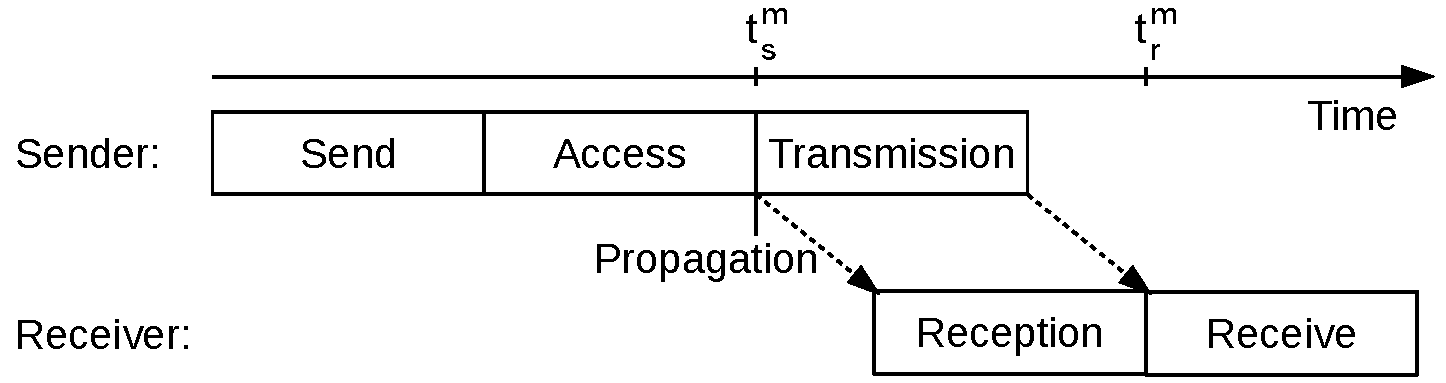
\includegraphics[width=0.75\textwidth]{images/time-synchronization/delays.pdf}
	\caption{Sources of delivery delays in the exchange of a message $m$ between two neighbor modules.\label{fig:time-sync:delay-decomposition}}
\end{figure}

% first introduced by Kopetz and 
%Ochsenreiter [7],[8] and later extended  in [3] and [5]
%\cite{kopetz1987clock} 

As indicated in~\cite{ganeriwal2003timing,maroti2004flooding,amundson2008time}, the exchange of a single message $m$ between two neighbor modules can be typically characterized by the steps presented in Figure~\ref{fig:time-sync:delay-decomposition}. Sending and receiving times represent the times necessary for the message to travel from the application to the data-link layers. These delays are introduced by the operating system and are highly non-deterministic. The access time represents the waiting time at the data-link layer for accessing the communication channel. This time is also highly non-deterministic. The transmission and reception times represent, respectively, the times to transmit and to receive the frame using a bit-by-bit transmission at the physical layer. These delays are mainly deterministic and depend on the length of the frame and the bitrate. The propagation time represents the time necessary for the bits to travel from the sender to the receiver over the physical link. This delay is highly deterministic and depends on the distance between the modules involved in the communication and on the propagation speed over the physical link. We define the transfer time, $T_{transfer}^m$, as the sum of the transmission, propagation and reception times for a message $m$. These times are highly deterministic.

\subsection{Predictive Method to Compensate for Communication Delays}
\label{section:time-sync:pred-method}

We propose to use the predictive method (PRED) to compensate for communication delays whenever they can be predicted. PRED is a naive method that relies on the assumption that $T_{transfer}^m$ is predictable with a certain accuracy that directly impacts the precision of our protocol. Moreover, it assumes that messages can be timestamped at the data-link layer, shortly before the beginning of the transmission at time $t_s^{m}$ and upon complete reception at time $t_r^{m}$. If we neglect the interrupt handling time, $T_{transfer}^m = t_r^{m} - t_s^{m}$.

To compensate for communication delays, the predictive method (PRED)  works as follows: Let us assume that a module $M_i$ receives a message $m$ from a module $M_j$ and that $m$ has been timestamped at the data-link layer on both sides (i.e., $m$ contains  $L^{M_j}(t_s^{m})$ and $L^{M_i}(t_r^{m})$). Then, the module $M_i$ can compensate for the communication delays of $m$ and estimate the local time of $M_j$ at the reception of $m$ by:
\begin{equation}
L^{M_j}(t_r^{m}) \approx L^{M_j}(t_s^{m}) + T_{transfer}^m
\end{equation}

\section{The Modular Robot Time Protocol}
\label{section:time-sync:protocol}

MRTP works in two steps. The first step initializes the system: election of a central module as the time master \textit{TM}, construction of a spanning tree and initialization of the global clock. In the second step, the time master periodically synchronizes the slave modules. 

\subsection{Method to Compensate for Communication Delays}

The method of compensating for communication delays in MRTP has to be carefully selected depending on the target system. The choice of this method has a direct impact on both the precision of the synchronization and its efficiency in terms of communications. The precision of an approach mainly depends on the hardware-clock precision, its resolution and the communication mechanism. In Section~\ref{section:time-sync:delay-comp-method}, we describe a procedure to experimentally evaluate the precision of a given approach over multiple hops.

In that section, we also show that, in our target system, i.e., the Blinky Blocks, PRED is on average more precise than the other two existing methods that can be applied to this system (i.e., FD and RTT). Moreover, PRED uses a unidirectional message exchange while RTT requires a bidirectional message exchange, thus incurring a larger communication overhead.

In the rest of this section, we describe MRTP, assuming PRED is used. Note that in practice, any method compatible with the target system can be used in MRTP.

\subsection{Step 1: Initialization}

\paragraph{Time Master Election}

A module is elected as the time master using an external algorithm. Different criteria can be used for the election of the time master (e.g., minimum-identifier node, etc.). Modular robotic systems with neighbor-to-neighbor communications form large-diameter networks (see Section~\ref{section:context:lmrs}). 

To achieve a better synchronization precision, we recommend electing a central module as the time master, i.e., a node that tends to minimize the maximum or the average hop distance to any other module. Placing the time master close to the center of the system reduces the time of the synchronization phases and increases the overall precision because cumulative estimations are made at every hop. Note that we do not claim that one can infer the synchronization precision of MRTP knowing the diameter of the target network. We only suggest a suitable position for the time master in a given system. Of course, the node density, the traffic distribution and the clock distribution may have an impact on the overall synchronization precision.

Any center election algorithm can be used to elect a central module. We suggest using one of the algorithms defined in the previous chapter ($k$-BFS SumSweep, ABC-Center or PC2LE) or the algorithm presented in~\cite{kim2013leader}. These algorithms scale well in terms of memory usage and execution time.

To handle dynamic topology changes, a module launches a time master re-election if it detects a new neighbor or a neighbor departure, and the system goes through the whole initialization process again.

\paragraph{Breadth-First Spanning Tree Construction}

At the end of the election process, our protocol creates a breadth-first spanning tree rooted at the time master. The \cheungCb{} algorithm, presented in Section~\ref{section:centrality:bfs}, can be used. This algorithm guarantees that modules at distance $d_{\mathrm{TM}}$ hops of the time master in the physical configuration, are at distance $d_{\mathrm{TM}}$ hops in the tree. Logical neighbors in the tree are neighbors in the physical configuration. At this point, every module knows its parent and children in the tree. This tree will be used to recursively propagate synchronization waves from the time master through the system. As explained in Section~\ref{section:synchronization:related-work:infrastructure}, this approach is, in compact systems running under our assumptions, more communication-efficient than infrastructure-less network-wide flooding based approaches.

\paragraph{Global Clock Initialization}

Initially, slave modules estimate the global time with their local time. Slave modules adjust their estimation of the global time during synchronization phases, in the second step of MRTP. When a new time master is elected, modules keep their previous estimation of the global time but do not keep the previous corrections of the clock skew. They can indeed disturb the synchronization process when two distinct systems are merged together.

Since time cannot run backward, clocks ahead of the global timescale have to slow down or to wait during the synchronization process, and clocks behind the global timescale have to jump to it. To make time synchronization faster, the global time, held by the time master, is initially set to an estimation of the most advanced global time in the system using the convergecast-max-time algorithm. Note that this approach can cause important jumps into the future.

\myAlg{
	\Input{
		$M_p$ \tcp{\footnotesize parent in the tree}\\
		\nonl{$Children$ \tcp{\footnotesize set of children in the tree}}
	}
	
	\BlankLine
	\BlankLine
	
	{\bf Initialization} of $M_i$ at time $t_{init}$:
	
	$offset \gets G^{M_i}(t_{init}) - L^{M_i}(t_{init})$; $Wait \gets Children$\;\label{alg:time-sync:convergecast:line:init}
	\uIf{$M_p = \perp$} {
		\ShowLn \tcp{\footnotesize convergecast-max-time terminates}\label{alg:time-sync:convergecast:line:end1}
	}
	\ElseIf{$Wait = \emptyset$} {
		send $m = $ BACK(\_,\_) to $M_p$\;\label{alg:time-sync:convergecast:line:parent1} 
		\tcp{\footnotesize $M_p$ will receive BACK($ Y^{M_i}(t_s^{m}) = L^{M_i}(t_s^{m}) + offset^{M_i}(t_s^{m}) ,L^{M_p}(t_r^{m})$) at the application layer. $Y^{M_i}(t_s^{m})$ is inserted by $M_i$ at the data-link layer, just before transmission start. $M_p$ will insert $L^{M_p}(t_r^{m})$ upon reception, at the data-link layer.
		}
	}
	
	\BlankLine
	\BlankLine
	{\bf When}  m = BACK($Y^{M_c}(t_s^{m}),L^{M_i}(t_r^{m})$) {\bf is received by} $M_i$
	{\bf from} $M_c$ such that $M_c \in Children$ {\bf do}:
	
	$Y^{M_c}(t_r^{m}) \gets Y^{M_c}(t_s^{m}) + T_{transfer}^{m}$\;	\label{alg:time-sync:convergecast:line:estimation}
	
	$offset \gets max(offset, Y^{M_c}(t_r^{m}) - L^{M_i}(t_r^{m}))$\label{alg:time-sync:convergecast:line:max}\;
	
	$Wait \gets Wait - \{M_c\}$\;
	\uIf{$M_p = \perp$} {
		\ShowLn \tcp{\footnotesize convergecast-max-time terminates}\label{alg:time-sync:convergecast:line:end2}
	}
	\ElseIf{$Wait = \emptyset$}{
		send $m' =$ BACK$(\_,\_)$ to $M_p$\; \label{alg:time-sync:convergecast:line:parent2}\tcp{\footnotesize As explain in comment line~\ref{alg:time-sync:convergecast:line:parent1}, $M_p$ will receive BACK($ Y^{M_i}(t_s^{m'}),L^{M_p}(t_r^{m'})$) at the application layer.}
	}
	\caption{The convergecast-max-time algorithm for a module, $M_i$.\label{alg:time-sync:convergecast}}
}

The pseudo-code of convergecast-max-time for any module $M_i$ is provided in Algorithm~\ref{alg:time-sync:convergecast}. At any time, a module $M_i$ estimates the maximum global time with:
\begin{equation}
Y^{M_i}(t) = L^{M_i}(t) + offset^{M_i}(t)
\end{equation}
with $offset^{M_i}(t)$ being the estimated offset between the estimation of ${M_i}$ concerning the maximum global time in the system and the local clock of ${M_i}$ at time $t$. Initially, ${M_i}$ considers it has the maximum global time (line~\ref{alg:time-sync:convergecast:line:init}). This algorithm uses a single type of message, namely \textit{BACK} message. Every \textit{BACK} message $m$ is timestamped twice at the data-link layer: the sender ${M_j}$ inserts $Y^{M_j}(t_s^{m})$ just before transmission starts and the receiver ${M_k}$ inserts $L^{M_k}(t_r^{m})$ upon complete reception (see Figure~\ref{fig:time-sync:delay-decomposition}).Each leaf module sends a \textit{BACK} message to its parent (line~\ref{alg:time-sync:convergecast:line:parent1}). Every non-leaf module waits for a \textit{BACK} message from all its children. When ${M_i}$ receives a \textit{BACK}$(Y^{M_c}(t_s^{m}),L^{M_i}(t_r^{m}))$ message $m$ from one of its children $M_c$, $M_i$ estimates $Y^{M_c}(t_r^{m}) \approx Y^{M_c}(t_s^{m}) + T_{transfer}^m$ using the PRED method (line~\ref{alg:time-sync:convergecast:line:estimation}) and adjusts $offset^{M_i}(t)$ accordingly (line~\ref{alg:time-sync:convergecast:line:max}). When ${M_i}$ has received a \textit{BACK} message from all its children, it sends in turn a \textit{BACK} message to its parent. When the convergecast terminates (lines~\ref{alg:time-sync:convergecast:line:end1} or~\ref{alg:time-sync:convergecast:line:end2}), the time master has an estimation of the maximum global time in the system $Y^{\mathrm{\textit{TM}}}(t)$. The time master then sets the global timescale $G(t)$ to $Y^{\mathrm{\textit{TM}}}(t)$. The convergecast-max-time algorithm neglects the effect of clock skew, and considers offsets to be constant in the system during convergecast.

\subsection{Step 2: Periodic Synchronization}

The time master holds the global timescale and periodically initiates synchronization phases. During each synchronization phase, the time master disseminates the current global time along the edges of the spanning tree built in the first step. $\tilde{G}(t)$, an estimation of the global time, is disseminated through the spanning tree, module-by-module, starting from the time master. At each hop, the transmitted time is updated to take into account communication delays and time of residence in intermediate modules. Slave modules use a linear model to compensate for clock skew. As explained in the related-work section, this is a common choice.

The time master starts a synchronization phase by sending the actual global time to all its children. Algorithm~\ref{alg:time-sync:synchronization} details the synchronization process of any slave module $M_i$.


\myAlg{
	\Input{
		$M_p$ \tcp{\footnotesize parent in the tree}\\
		\nonl{$Children$ \tcp{\footnotesize set of children in the tree}}\\
		\nonl{$w$ \tcp{\footnotesize maximum number of synchronization points used for linear regressions}}
	}
	
	
	\BlankLine
	\BlankLine
	
	{\bf Initialization} of $M_i$:
	
	$a \gets 1.0$; $b \gets 0$; $W \gets \emptyset$;\label{alg:time-sync:synchronization:line:init}
	
	\BlankLine
	\BlankLine
	{\bf When} m = SYNC($\tilde{G}(t_s^{m})$,$L^{M_i}(t_r^{m})$) {\bf is received by} ${M_i}$
	{\bf from} its parent ${M_p}$ {\bf do}:
	
	$\tilde{G}(t_r^{m}) = \tilde{G}(t_s^{m}) +
	T_{transfer}^m$\;\label{alg:time-sync:synchronization:line:estimation}
	\If{$|W| = w$}{ \label{alg:time-sync:synchronization:line:insertion:beginning}
		$W \gets W - \{\underset{\tilde{G}(t)} {\mathrm{argmin}}\ W(<\!\tilde{G}(t),L(t)\!>)\}$\;
	}
	$W \gets W\ \cup 
	<\!\tilde{G}(t_r^{m}),L^{M_i}(t_r^{m})\!>$\;\label{alg:time-sync:synchronization:line:insertion:end}
	computeLinearRegression($a,b,W$)\;\label{alg:time-sync:synchronization:line:regression}
	\ForEach{$M_c \in Children$ } {
		send $m' =$ SYNC$(\_,\_)$ to $M_c$\; \label{alg:time-sync:synchronization:line:dissemination} 
		\tcp{\footnotesize $M_c$ will receive SYNC($\small \tilde{G}(t_s^{m'}),L^{M_c}(t_r^{m'})$) at the application layer. $\tilde{G}(t_s^{m'}) = \tilde{G}(t_r^{m}) + a^{M_i}(W^{M_i}(t_s^{m'}))*(L^{M_i}(t_s^{m'}) - L^{M_i}(t_r^{m}))$ is inserted at the data-link layer, just before transmission start. $M_c$ will insert $L^{M_c}(t_r^{m'})$ upon reception, at the data-link layer.}
	}
	\caption{Synchronization protocol for a slave module, ${M_i}$.\label{alg:time-sync:synchronization}}
}

\paragraph{Time-stamping and Global Time Estimation}
\label{section:time-sync:synchronization-error}

The synchronization process uses a single type of message \textit{SYNC}. Every \textit{SYNC} message $m$ is timestamped twice at the data-link layer: the sender, ${M_j}$, inserts $\tilde{G}(t_s^{m})$ just before transmission starts and the receiver, ${M_k}$, inserts $L^{M_k}(t_r^{m})$ upon complete reception. When ${M_i}$ receives a \textit{SYNC}$(\tilde{G}(t_s^{m}),L^{M_i}(t_r^{m}))$ message $m$ from its parent, ${M_i}$ computes $\tilde{G}(t_r^{m}) = \tilde{G}(t_s^{m}) + T_{transfer}^{m}$, an estimation of the global time at the reception of the synchronization message, using the PRED method (line~\ref{alg:time-sync:synchronization:line:estimation}). $<\!\tilde{G}(t_r^{m}),L^{M_i}{(t_r^{m})}\!>$ forms a synchronization point that contains both the local clock value of $M_i$ and the estimation of the global time at nearly the same real time. ${M_i}$ can estimate its relative synchronization error with respect to the global time using Equation~\eqref{eq:time-sync:estimated-relative-error}.

\begin{equation}
	\label{eq:time-sync:estimated-relative-error}
	\tilde{\epsilon}^{M_i}(t) = G^{M_i}(t_r^{m}) - \tilde{G}(t_r^{m})
\end{equation}

\paragraph{Global Clock Adjustment}

$M_i$ computes $a^{M_i}(W^{M_i}(t))$ and $b^{M_i}(W^{M_i}(t))$ such that
\begin{equation}
\tilde{G}(t) \sim a^{M_i}(W^{M_i}(t))\times L^{M_i}(t) + b^{M_i}(W^{M_i}(t))
\end{equation}
using least-squares linear regression based on $W^{M_i}(t)$, a window of the last $w$ synchronization points (line~\ref{alg:time-sync:synchronization:line:regression}). $a^{M_i}(W^{M_i}(t))$ denotes the $M_i$ estimated skew with respect to the global time, and $b^{M_i}(W^{M_i}(t))$ its estimated offset at time $t$. This mechanism compensates for clock skew and enables modules to be synchronized less frequently without degrading the synchronization precision. In order to preserve time monotonicity, our protocol prevents $G^{M_i}(t)$ from running backward: 
\begin{equation}
%\small
\forall (t, t'), t \geq t', \ G^{M_i}(t) = \max{\left(G^{M_i}(t'),\ a^{M_i}\left(W^{M_i}(t)\right)\times L^{M_i}(t) + b^{M_i}\left(W^{M_i}(t)\right)\right)}
\end{equation}
If a new computed model leads to an estimated global time behind the maximum time already reached by $G^{M_i}(t)$, then $G^{M_i}(t)$ is blocked until the new model reaches this maximum time. Otherwise, $G^{M_i}(t)$ jumps into the future.

\paragraph{Global Time Dissemination}

${M_i}$ then sends a \textit{SYNC} message $m'$ to each of its children ${M_c}$ in the tree (line~\ref{alg:time-sync:synchronization:line:dissemination}). At the data-link layer, ${M_i}$ inserts 
\begin{equation}\tilde{G}(t_s^{m'}) = \tilde{G}(t_r^{m}) + a^{M_i}\left(W^{M_i}\left(t_s^{m'}\right)\right)\times \left(L^{M_i}\left(t_s^{m'}\right) - L^{M_i}\left(t_r^{m}\right)\right)
\end{equation} into $m'$, just before it starts to transmit the frame over the communication medium. This compensates for the time of residence at module ${M_i}$, assuming the ${M_i}$ clock skew to be constant and equal to $a^{M_i}(W^{M_i}(t_s^{m'}))$ during this time. ${M_c}$ inserts its local time $L^{M_c}(t_r^{m'})$ into the incoming message at the data-link layer, immediately after $M_c$ has pulled the synchronization message from the interface buffer. At the ${M_c}$ application layer, $m'$ contains $\tilde{G}(t_s^{m'})$ and $L^{M_c}(t_r^{m'})$. ${M_c}$ then repeats the same synchronization process as ${M_i}$.

\paragraph{Synchronization Periods}

%This scheme was suggested in~\cite{kusy2007spatiotemporal}.

Our protocol contains two synchronization phases: a calibration phase and a runtime phase. During the calibration phase, modules are more frequently synchronized with a period $P_{ca}$ in order to collect enough synchronization points to compute skew models while preserving a satisfying level of precision. The calibration phase lasts $w\times P_{ca}$. Then, during the runtime phase, modules are synchronized less frequently, with a period $P_{ru}$, and use the computed models to compensate for clock skew. The values of $w$, $P_{ca}$, and $P_{ru}$ have to be chosen according to the target platform hardware and the desired precision, with resource usage in mind.

In our experimental evaluation, we empirically selected $w = 5$, $P_{ca} = 2\ seconds$ and $P_{ru} = 5\ seconds$ (unless otherwise mentioned). These values provide, in our target platform, a satisfactory precision at a reasonable cost in terms of communications and computations.

\section{The Target System: the Blinky Blocks}
\label{section:time-sync:target}

We implemented MRTP and evaluated it on the Blinky Blocks system using both hardware prototypes and simulations on VisibleSim. Figure~\ref{fig:time-sync:mrtp-blinkyblocks} shows MRTP running on hardware Blinky Blocks. This section presents the characteristics of the Blinky Blocks local clocks and communication systems on the hardware prototypes along with the simulation models used in the simulations.

{
\newcommand{\ImgWidth}{4.5cm}
\newcommand{\ImgHeight}{4.5cm}
\begin{figure}[!h]
	\begin{center}
		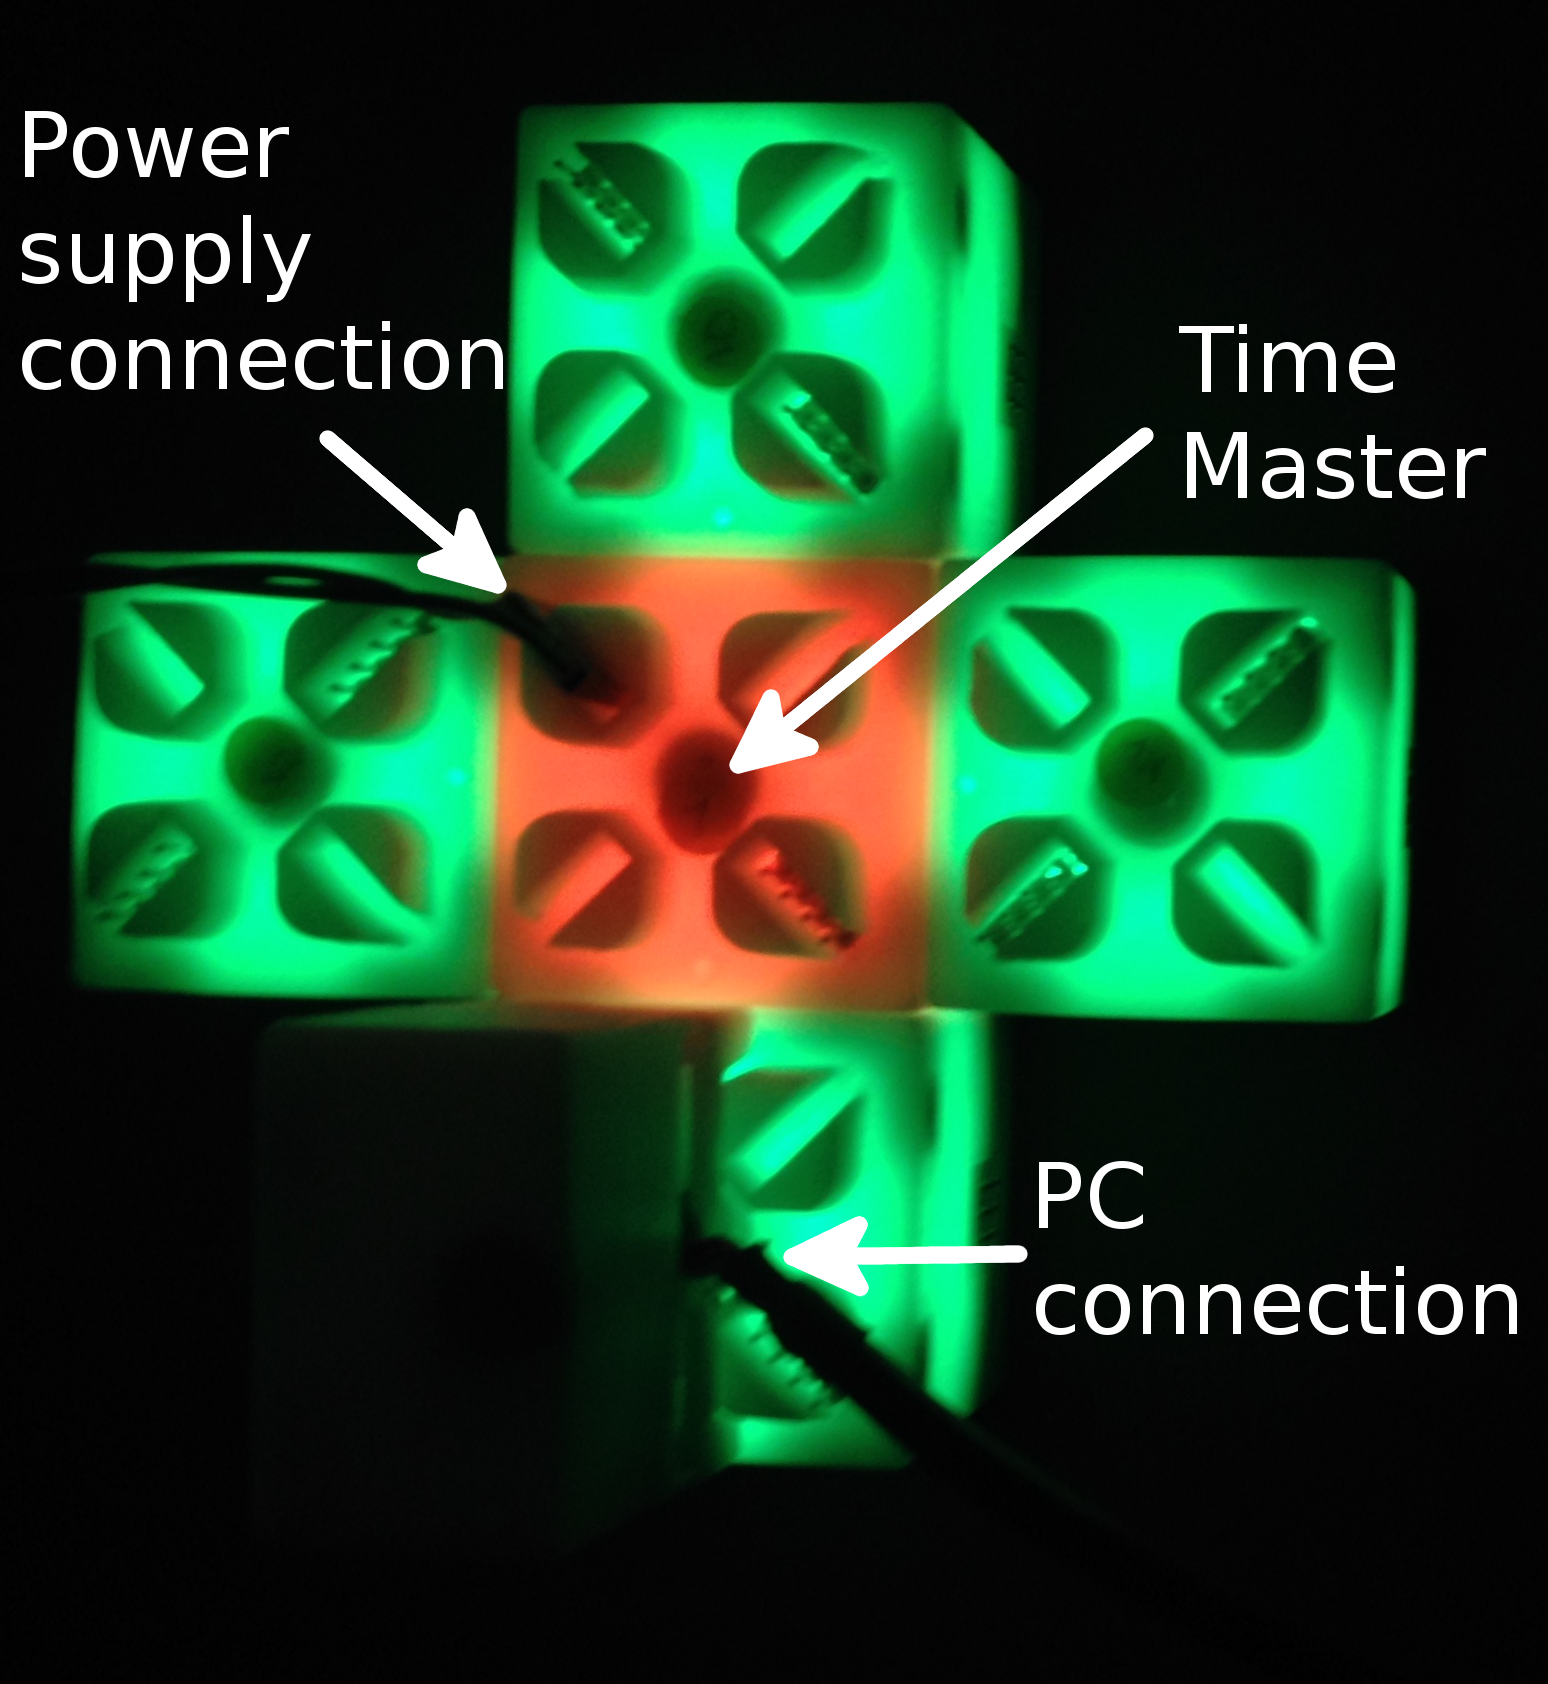
\includegraphics[width=\ImgWidth,height=\ImgHeight]{images/time-synchronization/cross.png}
		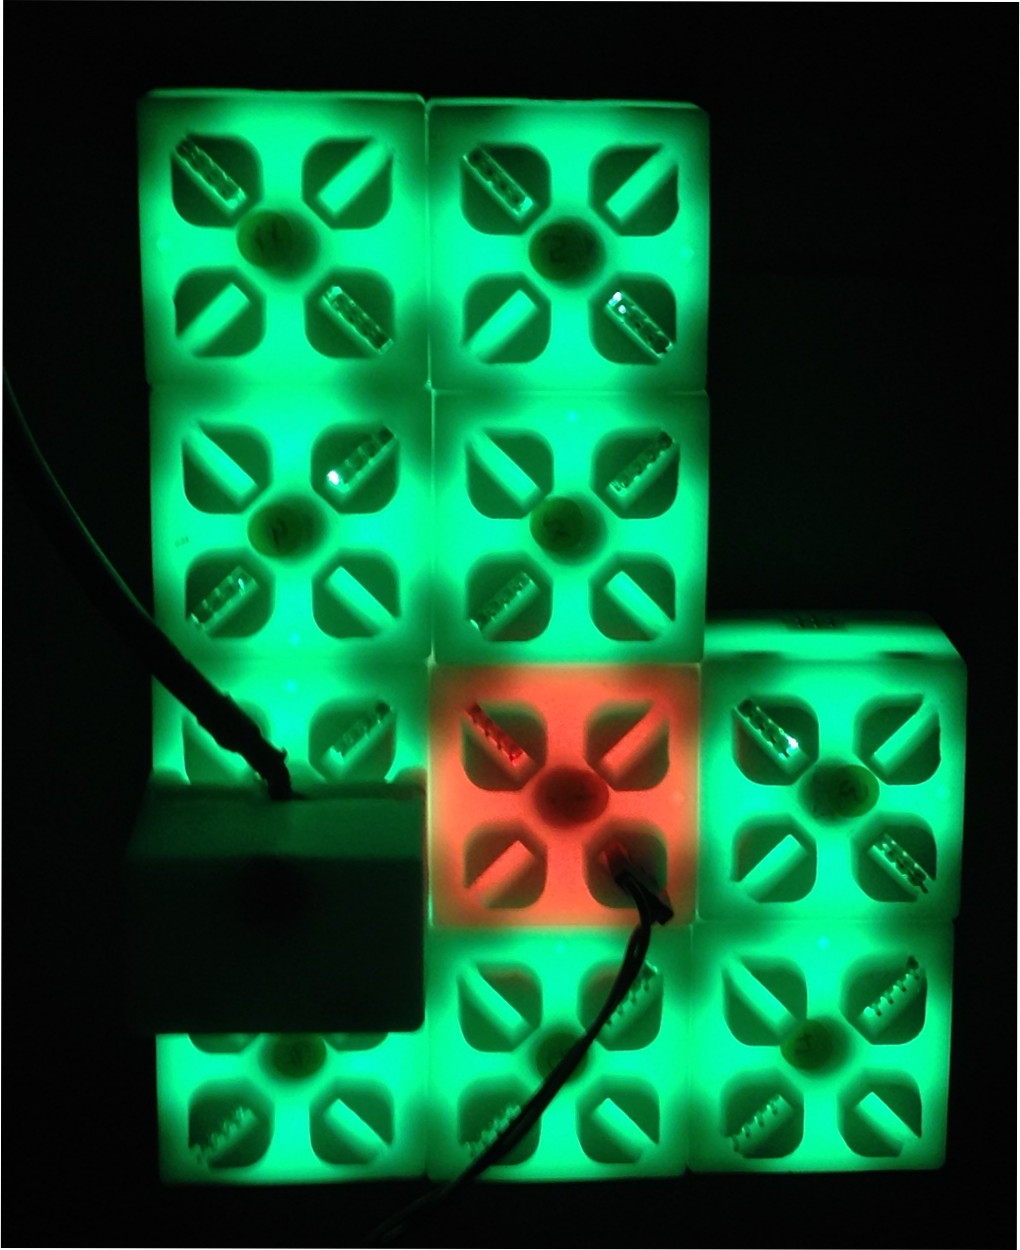
\includegraphics[width=\ImgWidth,height=\ImgHeight]{images/time-synchronization/L.png}
	\end{center}
	\caption{Two Blinky Blocks systems synchronized using MRTP. On the left, the system forms a cross. On the right, blocks are deployed in a doubled L-configuration. In both configurations, the time master, in red, is connected to the power supply. Slave modules are in green. Experimental data are sent by the systems to the PC through a serial cable.\label{fig:time-sync:mrtp-blinkyblocks}}
\end{figure}
}

\subsection{Local Clock Properties}

\paragraph{Hardware System}

Each module maintains its local time using a Real-Time Counter (RTC) driven by an internal RC oscillator running at a frequency of 1.024~kHz with an accuracy of 1\% (10,000 ppm), at 3V and 25\degree C \cite{avr1003}. The RTC counts the time elapsed since the module started with a resolution of about 0.98 millisecond\footnote{Resolution$ = \frac{1}{1.024} \approx 0.98 ms$}. Thus, the synchronization precision results announced in the evaluation section are actually expressed in 0.98 a millisecond, even though we express them in milliseconds for the sake of simplicity. It is important to understand that these oscillators exhibit a very poor accuracy and low resolution that directly affects the performance of our protocol. For instance, a frequency deviation of 1\% causes a clock error of approximately 10 milliseconds per second. Most previous work on time synchronization, e.g.,~\cite{elson2002fine,ganeriwal2003timing,maroti2004flooding,schenato2011average}, was evaluated on devices equipped with crystal oscillators that have a typical accuracy between 0.0001\% and 0.01\% (1 to 100 ppm) and a resolution in the order of tens of microseconds. Under constant temperature and constant supply voltage conditions, RC oscillators are fairly stable over a short period of time. As shown in Figure~\ref{fig:time-sync:deviation-real-time}, Blinky Blocks local clocks tend to drift apart in a roughly linear fashion in the short term.

\begin{figure}[h!]
	\centering
	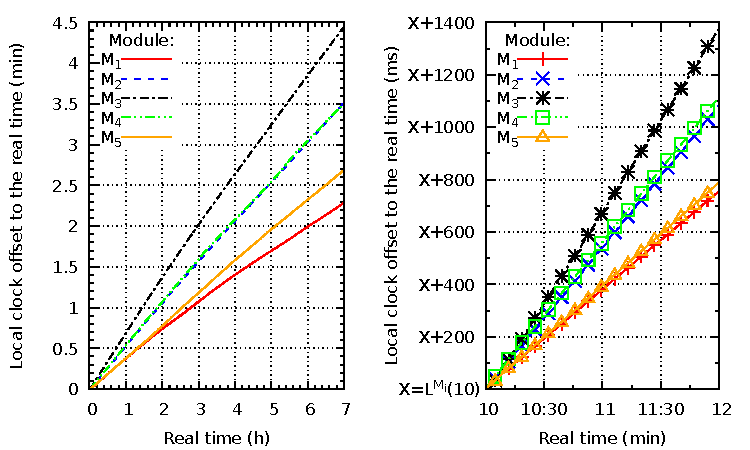
\includegraphics[width=0.7\linewidth]{images/time-synchronization/deviation-real-time}
	\caption{Local clock offset with respect to the real time $(L^{M_i}(t) - t)$. The plot on the left shows the long-term deviation of the local clocks, while the plot on the right shows these deviations in the shorter term. The PRED method was used to compensate for communication delays.}
	\label{fig:time-sync:deviation-real-time}
\end{figure}

\paragraph{Simulation Model}

In~\cite{allan1987time}, the authors propose a general model for oscillators:
\begin{equation}
L^{M_i}(t) = \frac{1}{2}D^{M_i}t^2 + y^{M_i}_0t + x_0^{M_i} + \eta^{M_i}(t)
\label{eq:oscillator-model}
\end{equation}
where $t$ is the real time (i.e., simulation time), $L(t)$ is the local time, $x_0$ is the time offset, $y_0$ is the frequency offset, $D$ is the frequency drift and $\eta(t)$ is a random noise. As explained in~\cite{allan1987time}, $y_0$ and $D$ may vary over time (e.g., due to aging, temperature variations, etc.). For the sake of simplicity, we consider them to be constant and express their small variations in the noise signal $\eta(t)$.

We assume that Blinky Blocks clocks follow the model shown in~\eqref{eq:oscillator-model}. We conducted experiments on hardware using Blinky Blocks in order to compute model parameters. We used a system of five blocks deployed in a cross configuration (see Figure~\ref{fig:time-sync:mrtp-blinkyblocks}) to collect time reference points $<t,L^{M_i}(t)>$, with $i$ being the block unique identifier, every 10 seconds during 7 hours (see Figure~\ref{fig:time-sync:deviation-real-time}). The real time $t$ was provided by a computer. We assumed the computer clock to be perfect. We use the PRED method of compensating for communication delays.

Figure~\ref{fig:time-sync:clock-parameters} shows the distribution of the parameter values obtained using polynomial regression with R. The parameters $D$ and $y_0$ seem normally distributed. As a consequence, we randomly generate clock parameters following normal distributions with the corresponding mean and standard deviation (see Table~\ref{table:time-sync:clock-parameters}). Noise signals are the residual standard errors. We extract the 5 noise signals and replay them in our simulations.

\begin{figure}[h!]
	\centering
	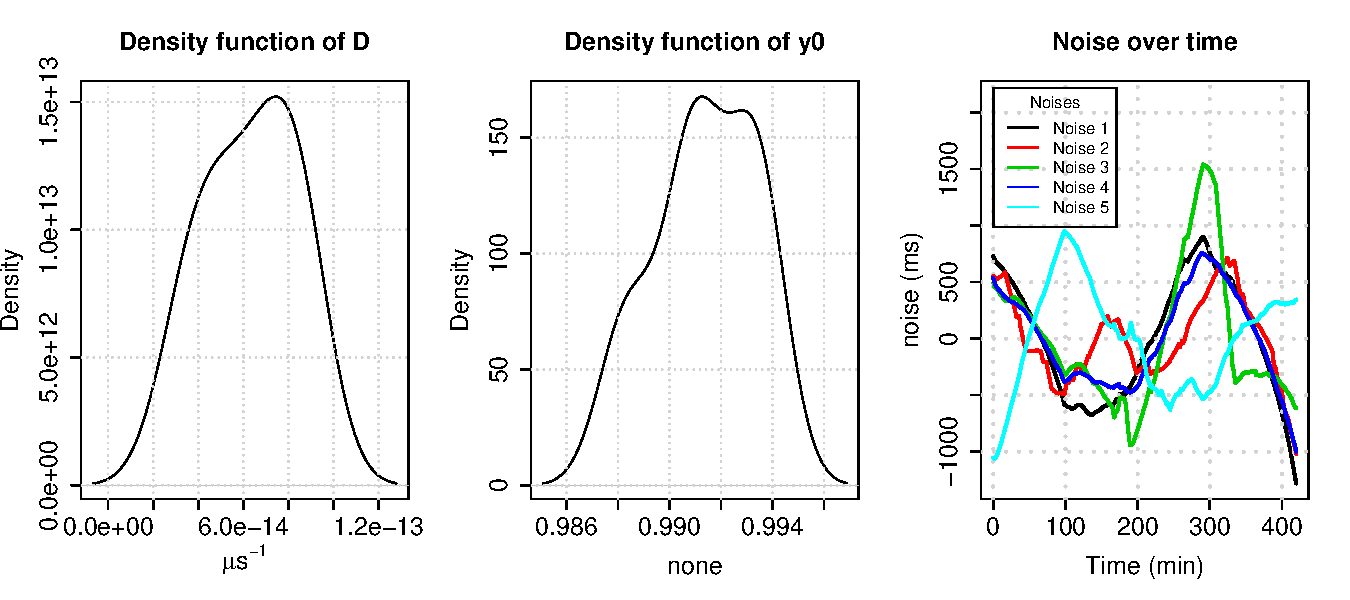
\includegraphics[width=\textwidth]{images/time-synchronization/parameters.pdf}
	\caption{Statistics on the parameters of the model used to simulate clocks. From left to right: $D$ density function, $y0$ density function and the noise signals over the time.}
	\label{fig:time-sync:clock-parameters}
\end{figure}

\begin{table}[h!]
	\begin{center}
		\small
		\begin{tabular}{|c|c|} 
			\hline
			Parameters & Simulation Model \\
			\hline
			$D\ (\mu s^{-1})$ & $\mathcal{N}(7.132315\times10^{-14},5.349995\times10^{-14})$ \\
			\hline
			$y_0\ (none)$ & $\mathcal{N}(0.9911011,0.002114563)$ \\
			\hline
			$x_0\ (\mu s)$ & additive inverse of the simulation time at module start-up \\
			\hline
			$\eta\ (\mu s)$ & Noise replayed from extracted data signals\\
			\hline	
		\end{tabular}		
		\caption{Blinky Blocks hardware-clock model parameters used in VisibleSim.  $\mathcal{N(\mu,\sigma)}$ refers to the normal probabilistic law, with $\mu$ being the mean and $\sigma$ the standard deviation.}
		\label{table:time-sync:clock-parameters}
	\end{center}
\end{table}

\subsection{Communication Properties}
\label{section:time-sync:communication-properties}

\paragraph{Hardware System}

We recall that Blinky Blocks use full-duplex neighbor-to-neighbor communications over serial links controlled by Universal Asynchronous Receivers/Transmitters (UARTs) configured with a bitrate of 38.4~kBauds. Modules exchange messages that contain up to 17~bytes of application data. A message is sent over the link into a frame composed of a minimum of 21~bytes: 17~bytes of payload data, 2~bytes for data related to message handling (active messaging~\cite{eicken1992active}) and 2~bytes of control (i.e., a frame delimiter byte and a checksum byte). Some special bytes need to be escaped using an extra byte in order to dissociate command bytes from data ones. Thus, the number of bytes actually sent on the link varies a little according to the data being sent.

A frame is transferred byte per byte to/from the UART. The transfer is interrupt-controlled, i.e., the UART generates an interrupt when it has finished transmitting or receiving a byte. The transmission time starts when the first byte of data is moved to the UART buffer and ends when the last byte leaves this buffer. The reception time starts when the first byte of data is received by the UART and ends when the last byte is received.

%At the application layer, modules exchange active messages~\cite{eicken1992active} that contains up to 17~bytes of data and a 2-byte handler function address. The handler is invoked on the receiver modules to handle the active message. At the data-link layer, every module maintains an outgoing-message queue per interface and a single incoming-message queue.

%Queued messages are processed in an interrupt-triggered system subroutine executed with a frequency of 2000 Hz (i.e., 500~us). During a call to this system subroutine, a module handles up to 6 messages from the incoming message queue and starts to send up to one message per interface. A message is sent over the link into a frame composed of 21~bytes minimum: 17~bytes of payload data and 4~bytes of control (i.e., frame delimiter, checksum, address of the handler function). Some special bytes need to be escaped using an extra byte in order to dissociate command bytes from data ones. Thus, the number of bytes actually sent on the link varies a little bit according to the data being sent. A frame is transfered byte per byte to/from the UART. The transfer is interrupt controlled, i.e., the UART generates an interrupt when it has finished transmitting or receiving a byte. The transmission time starts when the first byte of data is moved to the UART buffer and ends when the last byte leaves this buffer. The reception time starts when the first byte of data is received by the UART and ends when the last byte is received. Blinky Blocks use a protocol an ARQ (Automatic Repeat reQuest) protocol to deal with transmission failures, frames are transmitted up to 5 times.

%Well simulate need to look at the data link level because the number of bytes change => impact on the transfer time.

\paragraph{Transfer Time Estimation}

The PRED method used to compensate for communication delays assumes that the transfer time, defined in subsection~\ref{section:time-sync:msg-decomposition}, is predictable. The transfer time includes the transmission time, the propagation time and the reception time. The Blinky Blocks are identical and physically connected, thus the propagation time between two neighbor modules can be considered to be deterministic. The transmission time and the reception time of a message  depend on the actual frame size and on the communication rate. 

$T_{transfer}$ can be estimated using two-way timestamped-message exchanges (see Figures~\ref{fig:time-sync:transfer-time-1}-\ref{fig:time-sync:transfer-time-2} and Equation~\eqref{equation:transfer-time}). Equation~\eqref{equation:transfer-time} assumes the communication delays for frames of same size to be symmetrical. In addition, the exchange of messages is assumed to be fast enough so that the skew between the clock of the two modules is insignificant during the exchange.

{
	\begin{equation}
	\label{equation:transfer-time}
	T_{transfer} \approx \frac{(L^{M_2}(t_r^{m'}) - L^{M_2}(t_s^m)) - (L^{M_1}(t_s^{m'})-L^{M_1}(t_r^m))}{2}
	\end{equation}
}


\begin{figure}[h!]
	\centering
	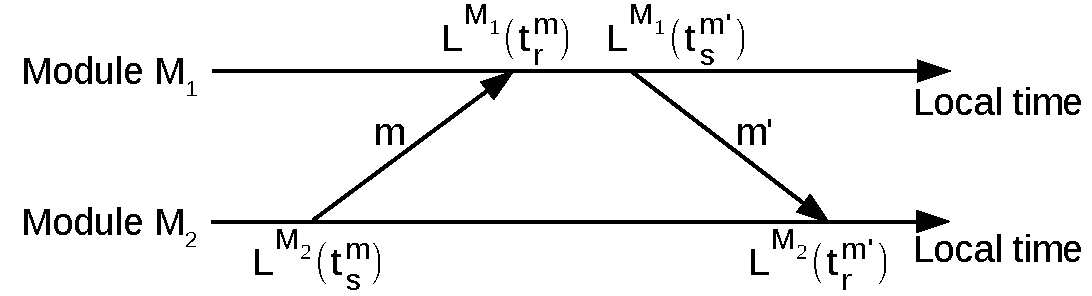
\includegraphics[width=0.6\textwidth]{images/time-synchronization/transfer.pdf}
	\caption{Scheme of a two-way message exchange between two blocks.}
	\label{fig:time-sync:transfer-time-1}
\end{figure}

\begin{figure}[h!]
	\centering
	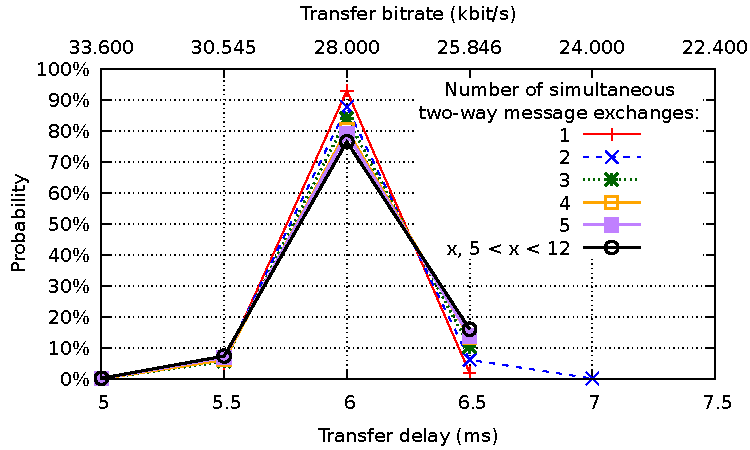
\includegraphics[width=0.7\textwidth]{images/time-synchronization/delayNeighborhood-article.pdf}	
	\caption{Transfer delay/rate distribution of 21-byte-long frames.}
	\label{fig:time-sync:transfer-time-2}
\end{figure}

We experimentally measured $\widetilde{T}_{transfer}$ for 300,000 two-way message exchanges between neighbor modules in sparse and compact Blinky Blocks systems (see Figure~\ref{fig:time-sync:transfer-time-2}). We observed that $\widetilde{T}_{transfer}$ is always between 5 and 7 milliseconds. On average, $\widetilde{T}_{transfer}$ of 21-byte long frames varies slightly around 6 milliseconds, depending on the number of simultaneous communications. Moreover, at the resolution of 1 millisecond, the transfer time of identical-length frames is fairly constant. A transfer time of 6 milliseconds for a 21-byte long frame corresponds to a transfer rate of 28 kbit/s. Based on these results, we consider that the transfer rate of a message can be estimated by $\widetilde{R}_{transfer} = 28\ kbit/s$. As a consequence, we use Equation~\eqref{equation:transfer-time-model} to estimate the transfer delay of a message and to compensate for communication delays in the PRED method.

\begin{equation}
\widetilde{T}_{transfer} = \frac{\text{frame size}}{\widetilde{R}_{transfer}}
\label{equation:transfer-time-model}
\end{equation}

\paragraph{Simulation Model}
\label{section:time-sync:network-simulation-model}

In order to accurately simulate the time, our simulation model takes into account the timeout triggering time, the processing time, the queueing delays, and the transfer rate of the messages (see Figure~\ref{fig:time-sync:comm-model}). We did not observe any node crash or any transmission failure or message loss during the experiments of the previous subsection, when the network is not overwhelmed. Thus, our simulation model does not incorporate any special mechanism to mimic such phenomena. Table~\ref{table:time-sync:comm-model} summarizes the different random variables of our model.

\begin{figure}[h!]
	\centering
	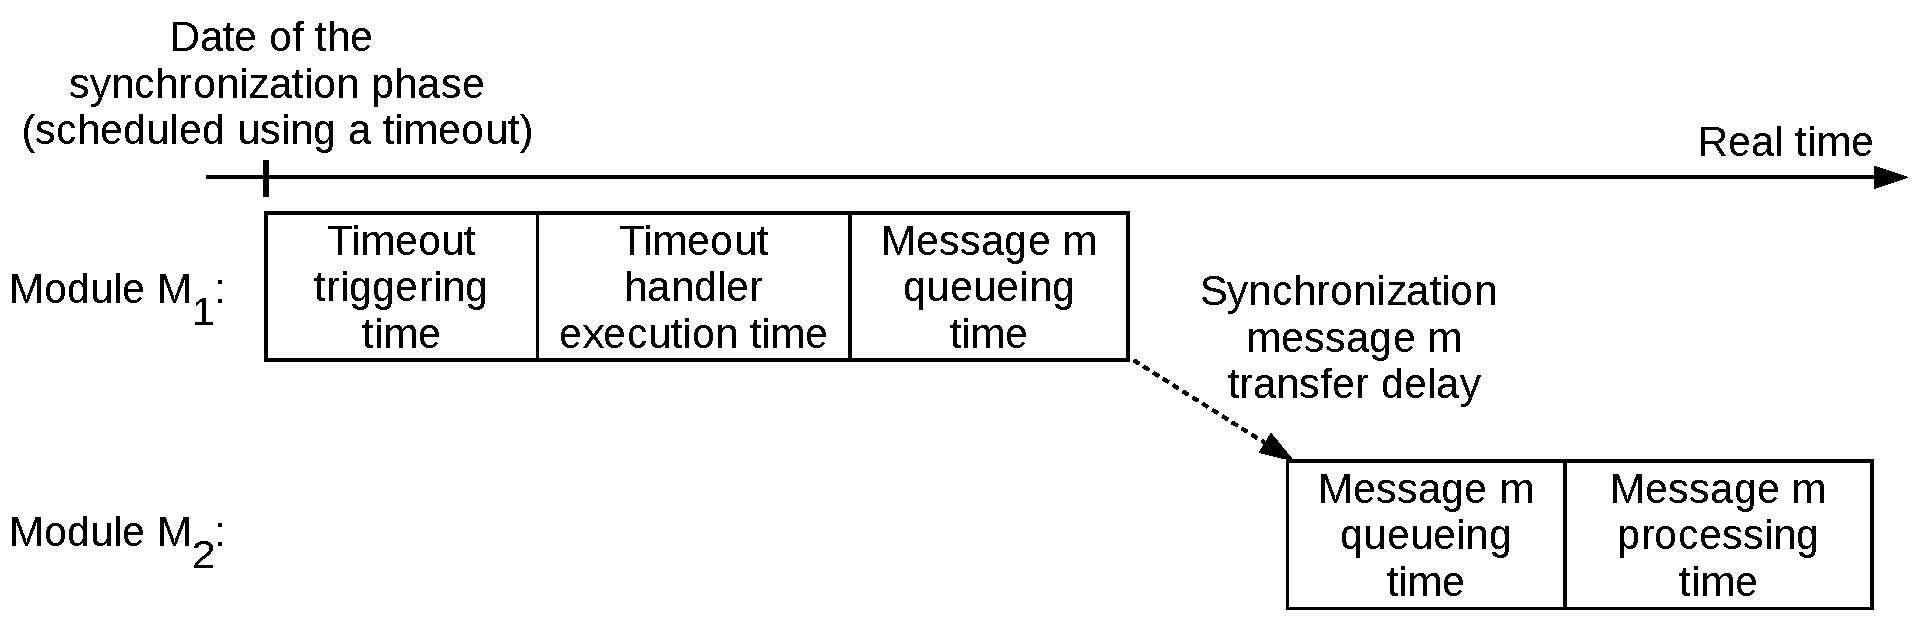
\includegraphics[width=0.9\linewidth]{images/time-synchronization/communication-model}
	\caption{Workflow of the communication model used for the simulation of time synchronization protocols. In this example, module $M_1$ has scheduled a synchronization phase. Upon timeout expiration, module $M_1$ executes the synchronization procedure and sends a synchronization message to module $M_2$ which will process it after a possible delay due to queueing.}
	\label{fig:time-sync:comm-model}
\end{figure}

\paragraph{Timeout triggering time}

The timeout triggering time is the amount of time a module needs to trigger an action scheduled using a software timeout (e.g., the synchronization timeout that initiates a synchronization phase). In the Blinky Blocks firmware, software timeouts are checked with a frequency of 2000~Hz. Thus, if we neglect the interrupt delay, an action scheduled at time $t$ can be executed at any time $t'$, such that $t \leq t' \leq t + 500\mu s$. 

\paragraph{Processing time}
We use the micro-controller clock running at 32~MHz (nanosecond scale resolution) to measure the processing time of the synchronization-timeout handler and the synchronization-message handler. We define two generic models to simulate the message-handler processing time: one for handlers with low-computation cost (e.g., clock adjustment without linear regression) and one for handlers with medium-computation cost (e.g., clock adjustment with linear regression computation on a window of 5 measures).

Note that the queueing and transfer delays include some processing time. In our evaluation, modules were running a rather simple application, in which every module periodically changes its color based on the current global time and does nothing the rest of the time using an active sleep (while loop with a time limit). Thus, they were actually computing all of the time.  The transfer time includes the interrupt time to fetch bytes from the interface buffer. Our target platform (and many others) uses interrupt-driven communications. Hence, only a very few elementary micro-controller instructions are executed before a byte is fetched. We reasonably assume that interrupts are never disabled and that there are not a large number of interrupts to be simultaneously handled. The queueing delays include interrupt time to enter the routine that handles incoming messages and the time to handle potential messages that were already present in the queue at the message arrival.

\paragraph{Queueing delays and network load}
%Network traffic modeling and queueing theory are beyond the scope of this paper.
VisibleSim uses a queueing system to handle both incoming and outgoing messages. We propose two queue load models. The first model is dedicated to lightly loaded networks where modules only exchange neighborhood management messages, with a period of 500 milliseconds. The second model is intended to simulate moderate network traffic due to extra-applications running on the nodes. In this model, in addition to simulating the neighborhood management messages, the queue occupancy at a message arrival follows a Poisson distribution of mean~1. This simulates a moderate network traffic in which message queues contain, most of the time, 0 to 2 messages and in a few cases more messages. The light-load model is used in the experiments of subsection~\ref{section:time-sync:hardware-eval}. The moderate-load model is used in our evaluation on large-scale systems (see Section~\ref{section:time-sync:large-scale-evaluation}).

\paragraph{Transfer rate}
Below the millisecond unit, the transfer rate is scenario-dependent. It depends, for instance, on the number of simultaneous communications. For each experiment performed on the hardware platform, we empirically derive the average system transfer rate using statistics on the round-trip time. We use similar experiments to the ones presented in subsection~\ref{section:time-sync:delay-comp-method}. We define three transfer rate models, namely for sparse, intermediate and compact systems. In a given simulation, all the modules use the same transfer rate model. The model for sparse systems is used in the experiments of subsection~\ref{section:time-sync:delay-comp-method}, on the line system. The model for intermediate systems is used in the experiments of subsections~\ref{section:time-sync:eval-period}~and~\ref{section:time-sync:eval-window}, on the L-shaped system (see Figure~\ref{fig:time-sync:mrtp-blinkyblocks}). The model for compact systems is used in our evaluation on large-scale systems (see Section~\ref{section:time-sync:large-scale-evaluation}).

{
	\newcommand{\lenOneTwo}{0.12\linewidth}
	\newcommand{\lenTwoTwo}{0.14\linewidth}
	\newcommand{\lenThreeTwo}{0.21\linewidth}
	\newcommand{\lenFourTwo}{0.30\linewidth}
	\begin{center}
		\begin{table}[h!]
			\centering
			\small
			\begin{tabular}{|C{\lenOneTwo}|C{\lenTwoTwo}|C{\lenFourTwo}|C{\lenFourTwo}|}
				\hline
				\multicolumn{3}{|c|}{Parameters} & Value\\
				\cline{1-4}
				\multirow{2}{*}{Timeouts} & \multicolumn{2}{c|}{Triggering time $(s)$} & $\mathcal{U}(0,500\times10^{-6})$\\
				\cline{2-4}
				& \multicolumn{2}{c|}{Processing time $(s)$} & $\mathcal{U}(250\times10^{-6},300\times10^{-6})$ \\
				\cline{1-4}
				\multirow{12}{*}{Messages} &
				\multirow{3}{*}{\begin{minipage}{\linewidth}\centering Queue occupancy at arrival \end{minipage}} &  Light load & neighborhood management \\
				\cline{3-4}
				& & Moderate load & neighborhood management +  $\mathcal{P}(1)$ \\
				\cline{2-4}
				& \multirow{6}{*}{\begin{minipage}{\linewidth}\centering Transfer rate $(kbit/s)$\end{minipage}} &  Sparse systems (e.g., line system) & $\mathcal{N}(28.134,0.660)$ \\
				\cline{3-4}
				& & Intermediate systems (e.g., L-shaped systems) & $\mathcal{N}(28.085,0.938)$ \\
				\cline{3-4}
				& & Compact systems (e.g., ball systems)& $\mathcal{N}(27.696,1.143)$ \\
				\cline{2-4}
				& \multirow{2}{*}{\begin{minipage}{\linewidth}\centering Processing time $(s)$\end{minipage}} & Low complexity & $\mathcal{U}(250\times10^{-6},300\times10^{-6})$ \\
				\cline{3-4}
				&  & Medium complexity& $\mathcal{U}(475\times10^{-6},525\times10^{-6})$\\
				\hline
			\end{tabular}
			\caption{Communication model used for the evaluation of time synchronization protocols. $\mathcal{N}(\mu,\sigma)$ refers to the normal probabilistic law, with $\mu$ being the mean and $\sigma$, the standard deviation. $\mathcal{U}(l,u)$ refers to the uniform probabilistic law with the minimum value $l$ and the maximum value $u$. $\mathcal{P}(\lambda)$ refers to the Poisson probabilistic law with $\lambda$ mean.}\label{table:time-sync:comm-model}
		\end{table}
	\end{center}
}

\section{Experimental Evaluation}
\label{section:time-sync:evaluation}

This section presents our experimental evaluation of MRTP, performed both on hardware Blinky Blocks and in the VisibleSim simulator. Through our experiments, we show the effectiveness, the efficiency and the scalability of our protocol. More precisely, we first evaluate the precision of MRTP on hardware and show through some examples that VisibleSim accurately simulates Blinky Blocks systems. Then, we use VisibleSim to evaluate the performance of MRTP in large-scale systems and to compare it to existing synchronization protocols in terms of precision, time of convergence and communication efficiency. Unless otherwise mentioned, we use the PRED method to compensate for communication delays in MRTP.

\subsection{Evaluation on Hardware and Validation of VisibleSim}
\label{section:time-sync:hardware-eval}

In this subsection, we evaluate the precision of the synchronization achieved by MRTP on the Blinky Blocks hardware. In addition, we show that VisibleSim accurately simulates Blinky Blocks systems. 

\subsubsection{Methodology}

We first use color changes to show that MRTP can potentially manage systems composed of up to 27,775 Blinky Blocks. 

Then, we show how the hop distance impacts the precision of the estimated global time $\tilde{G}(t)$ disseminated through the network during synchronization phases. We compare different methods to compensate for communication delays and show that the PRED method is on average the most accurate in our target platform. Furthermore, we show that within a few hops, $\tilde{G}(t)$ can be used as a reference time to estimate the relative synchronization error of the Blinky Blocks with respect to the global time. The relative synchronization error can thus be estimated using Equation~\eqref{eq:time-sync:estimated-relative-error}. 

We then use this estimation to study the local clock behaviors and to show the impact of various parameters on the precision of our protocol.

All experiments presented in this subsection were one-hour long. Unless otherwise mentioned, modules were synchronized every 2 seconds in the calibration phase, then every 5 seconds in the runtime phase and modules used five synchronization points for the linear regressions. These values were empirically chosen with the aim of obtaining, a satisfactory synchronization precision in practice, at reasonable computation and communication costs.

\subsubsection{Evaluation of the Precision of MRTP using Color Changes}
\label{section:time-sync:color-changes}

Measuring clock offsets using message exchanges is as challenging as performing time synchronization because time keeps going during communications.

In this subsection, we apply MRTP to a system of 28 Blinky Blocks\footnote{At the time of the evaluation of MRTP, we only had at our disposal 28 hardware Blinky Blocks.} that have to simultaneously change their color. Potential delays between module color changes reflect the synchronization error of the modules. Modules are connected in a line topology. The time master is manually placed at an extremity of the system and it synchronizes the other modules every 500 milliseconds. With a such runtime synchronization period, every link of the synchronization tree is theoretically used by MRTP only about $1.2\%$ of the time\footnote{$\frac{T_{transfer}}{P_{ru}} \approx \frac{6}{500} \approx 1.2\%$ (without retransmission due to potential message loss or corruption)}. Slave modules have to simultaneously change their color every 3 seconds. This experiment was recorded using a 40-millisecond-resolution camera.

We observed that every time the system started to change its color, all slave modules changed their color in the next image, 40 milliseconds later (see Figure~\ref{fig:time-sync:line}). Hence, MRTP is potentially able to synchronize a system with a radius of up to 27 hops to a less than 40 milliseconds, if the time master is at the center of that system. To give an order of magnitude, a Blinky Blocks system with a radius of 27 hops can be composed of up to 27,775 modules and have a diameter of 54 hops (using formulas demonstrated in Section~\ref{section:appendixLMRs:diameter-blinkyblocks}).

\begin{figure}[h!]
	\begin{center}
		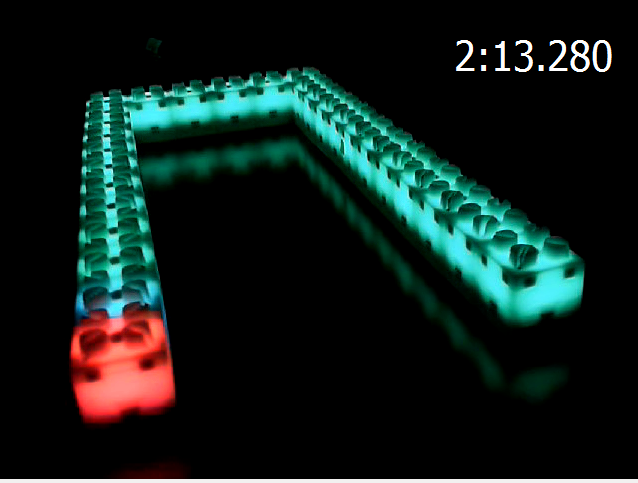
\includegraphics[width=0.35\textwidth]{images/time-synchronization/line1.png}
		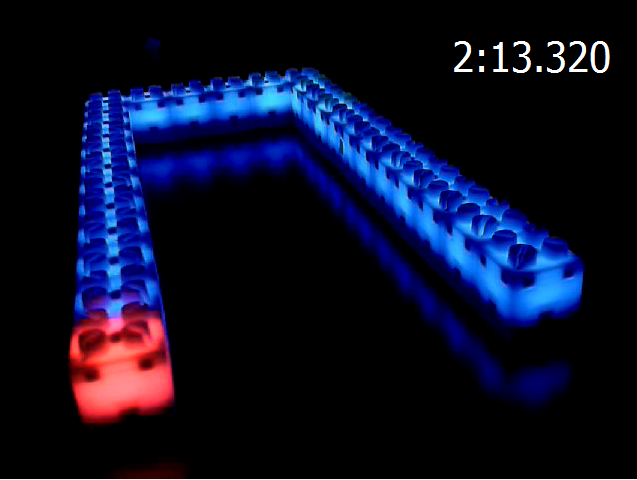
\includegraphics[width=0.35\textwidth]{images/time-synchronization/line2.png}
	\end{center}
	\caption{Two successive images of a video recording 28 Blinky Blocks connected in a line topology. The time master is in red. Slave modules have to simultaneously change their color every 3 seconds. On the left, a color change starts in the system. On the right, 40 milliseconds later, the color of every slave module has changed.\label{fig:time-sync:line}}
\end{figure}

In the next subsections, we present a more precise and automated evaluation of MRTP. 

\subsubsection{Impact of the Hop Distance and the Method to Compensate for Communication Delays on the Precision of the Disseminated Global Time $\tilde{G}(t)$}
\label{section:time-sync:delay-comp-method}

We expect that the estimation of the global time, $\tilde{G}(t)$, disseminated during the synchronization phases gets less precise as the depth of the synchronization tree increases because small but cumulative errors in the estimation of the global time are made at every hop. In this section, we first propose a generic method to evaluate compensation delay methods over multiple hops. Then, we present results obtained using the FD, RTT and PRED methods of compensating for communication delays (see Sections \ref{section:time-sync:communication-delay-comp-methods} and \ref{section:time-sync:pred-method}). We show that the PRED method is on average more accurate. Finally, we show that within a few hops, $\tilde{G}(t)$ can be used as a reference time to estimate the synchronization error of the Blinky Blocks.

\paragraph{Methodology}

We evaluate the precision of $\tilde{G}(t)$ using virtual modules emulated on Blinky Blocks hardware systems. Figure~\ref{fig:time-sync:virtual-line} gives the intuition behind our experiments in a line system. This method, inspired by the approach presented in~\cite{romer2005time}, allows us to compare the estimated global time received by the module $M_{2n-1}$ to the actual global time held by the time master $\mathrm{\textit{TM}}  = M_1$, because these two modules are emulated on the same physical block and can both read the actual global time $G(t)$. 

In the example depicted in Figure~\ref{fig:time-sync:virtual-line}, every physical block hosts 2 virtual modules, except for one block. Each slave virtual module maintains its own estimation of the global time. The synchronization tree rooted at the time master \textit{TM} links the virtual modules together in a virtual line, so that neighbor modules in the tree are hosted on a separate physical block. The leaf module $M_{2n-1}$ is at a distance of $2(n-1)$ hops from \textit{TM} in the synchronization tree. $M_{2n-1}$ computes the global-time dissemination error as $G(t) - \tilde{G}(t)$.

In our experiments, we generalize the example of the virtual line to measure the global-time dissemination error versus the hop distance in arbitrary systems. Modules host a number of virtual modules equal to the diameter of the system, and every physical module initiates a return trip to the root of the tree. The root of the tree receives timing messages that have physically traveled from 2 hops to $2(d-1)$ hops (or $2d-1$, if the diameter is odd). 

\begin{figure}[h!]
	\begin{center}
		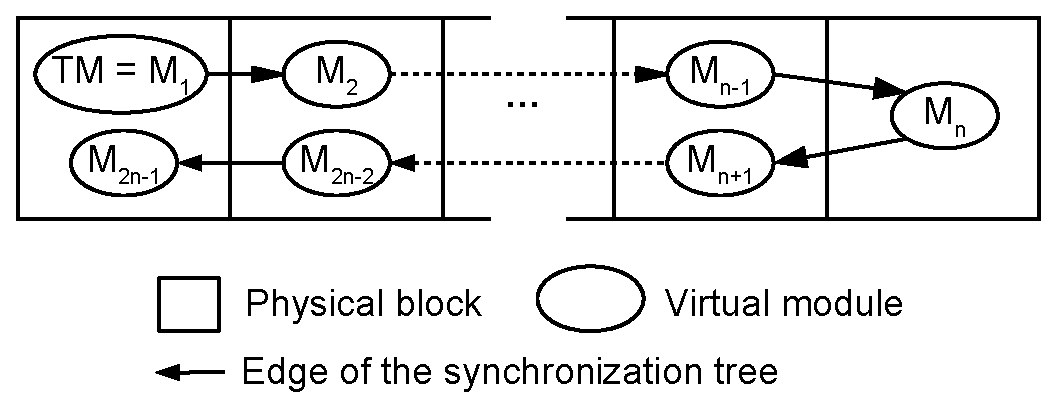
\includegraphics[width=0.7\textwidth]{images/time-synchronization/virtual-line.pdf}
	\end{center}
	\caption{Scheme of a virtual line of emulated modules on hardware Blinky Blocks connected in a line.}
	\label{fig:time-sync:virtual-line}
\end{figure}

\paragraph{Results}

Figure~\ref{fig:time-sync:dissemination-error} and Table~\ref{table:time-sync:diss-error} show the impact of the hop distance on the global-time dissemination error. As expected, the precision of the disseminated global time decreases with the hop distance. As stated in Section~\ref{section:time-sync:time-master}, the absolute mean error increases linearly with the number of hops and the standard error tends to increase with the square root of the number of hops. As a consequence, placing the time master at the center of the system appears to be a judicious choice.

\begin{figure}[!h]
	\begin{center}
		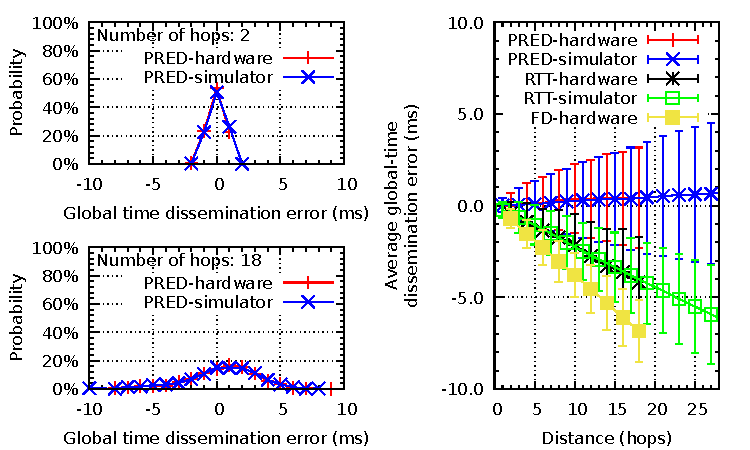
\includegraphics[width=0.75\textwidth]{images/time-synchronization/dissemination-error.pdf}
	\end{center}
	\caption{Global time dissemination error ($\pm$ standard deviation) in MRTP according to the hop distance. On the left, the distribution of the error. On the right, the average error ($\pm$ standard deviation).}
	\label{fig:time-sync:dissemination-error}
\end{figure}


{
	\newcommand{\lenOne}{0.19\linewidth}
	\newcommand{\lenTwo}{0.15\linewidth}
	\begin{center}
		\begin{table}[h!]
			\small	
			\begin{tabular}{|C{\lenOne}|C{\lenTwo}|C{\lenTwo}|C{\lenTwo}|C{\lenTwo}|}
				\hline
				& \multicolumn{4}{c|}{Average global-time dissemination error (ms)}\\
				\cline{2-5}
				Compensation & \multicolumn{2}{c|}{Line configuration} & \multicolumn{2}{c|}{Compact configuration} \\
				\cline{2-5}
				delay method & 2 hops & 4 hops & 2 hops & 4 hops \\
				\hline				
				PRED & $-0.03 \pm 0.70$& $-0.11 \pm 1.11$ & $-0.27 \pm 0.67$ & $-0.36 \pm 1.02$  \\
				\hline
				RTT & $-0.42 \pm 0.62$ & $-0.88 \pm 1.01$  & $-0.50 \pm 0.63$ & $-0.80 \pm 0.97$  \\
				\hline
				FD & $-0.71 \pm 0.50$ & $-1.53 \pm 0.76$ & $-0.87 \pm 0.54$ & $-1.63 \pm 0.80$ \\
				\hline
			\end{tabular}
			\caption{Average dissemination error ($\pm$ standard deviation) with respect to the global time in MRTP for 2 and 4 hops using different methods of compensating for communication delays in the line and the compact systems.}
			\label{table:time-sync:diss-error}
		\end{table}
	\end{center}
}

It appears that PRED is on average more precise than FD and RTT methods in sparse and more compact systems. We observe that regardless of the distance, the error distribution of PRED seems Gaussian and nearly centered around zero. This is mainly due to the fact that, in Blinky Blocks systems, the average transfer delay of a frame is almost a round number at the millisecond scale.

Note that PRED has a more important standard deviation than the other two methods.  FD has the smallest standard deviation as only the transfer time of a single byte is involved in the estimation of the global time whereas PRED and RTT use the transfer time of complete messages. In future work, it would be interesting to evaluate the performance of FD combined with a method that would compensate for the dissemination error only after several hops when this error has become greater than the resolution of the clock and can effectively be compensated for. From now, we only consider the PRED method for the evaluation on hardware.

For a distance of 4 hops, 95\% of the error measures are between [-2;2] milliseconds and the average error is close to zero. Because of the poor accuracy of the Blinky Blocks hardware clocks, we expect synchronization error using our protocol to be greater than 1 to 2 milliseconds. Thus, within a few hops, $\tilde{G}(t)$ can be used as a reference time to estimate the synchronization error of the Blinky Blocks. Upon reception of a synchronization message, a module ${M_i}$ estimates its relative synchronization error with respect to the global time by $\tilde{\epsilon}^{M_i}(t) = G^{M_i}(t) - \tilde{G}(t)$. We do not use virtual modules any more in the rest of the evaluation.

\subsubsection{Analysis of the Local Clock Behavior and Impact of the Hardware Clock Stability on the Synchronization Precision}

We measured the clock values of five blocks deployed in the cross-configuration depicted in Figure~\ref{fig:time-sync:mrtp-blinkyblocks}. The slave modules, denoted $M_6$, $M_7$, $M_8$ and $M_9$, ran under the same conditions: they were all synchronized using the same parameters and they were all neighbors of the time master which was connected to the power supply. Note that the physical modules used in these experiments differ from the ones used in Section~\ref{section:time-sync:target} to compute our simulation model. As shown in Figure~\ref{fig:time-sync:hardware-instability-density}, local clocks seem to drift apart from the global time in a roughly linear fashion. As indicated in Table~\ref{table:time-sync:clock-skew-statistics}, using linear models to compensate for clock skew significantly increases the synchronization precision. 

\begin{figure}[h!]
	\begin{center}
		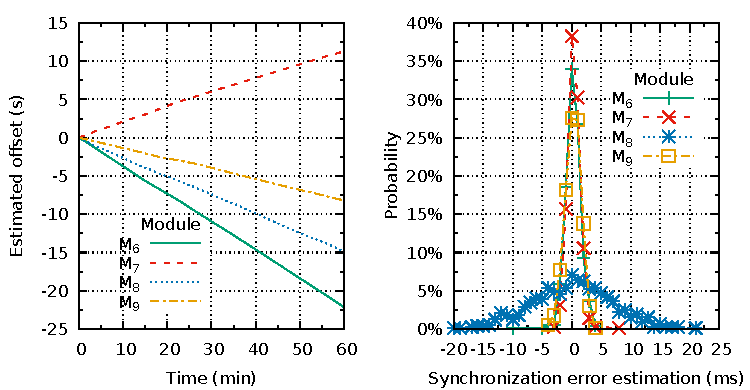
\includegraphics[width=0.7\textwidth]{images/time-synchronization/stability-results.pdf}
	\end{center}
	\caption{On the left, the estimated clock offset ($L^{M_i}(t) - \tilde{G}(t)$). On the right, the distribution of the relative synchronization error in MRTP.\label{fig:time-sync:hardware-instability-density}}
\end{figure}

\begin{table}[!h]
	\centering
	\small
	\begin{tabular}{|c|c|c|c|}
		\hline
		Clock skew & Average & Standard deviation & Maximum absolute \\
		compensation & (ms) & (ms) & (ms)\\
		\hline
		Linear model & 0.22 & 3.55 & 21 \\
		\hline
		None & -12.13 &  18.05 & 67 \\
		\hline
	\end{tabular}
	\caption{Statistics on the average relative synchronization error of the whole system showing the impact of using linear models to compensate for clock skew in MRTP.\label{table:time-sync:clock-skew-statistics}}
\end{table}

The distributions of the estimated relative synchronization errors observed for all blocks are shown in Figure~\ref{fig:time-sync:hardware-instability-density}. The distributions seem to be Gaussian. They are bell-shaped and nearly centered around 0. All modules remain synchronized to a few milliseconds.

However, it must be noted that the distribution for $M_8$ is much more spread out than the others. It is shorter and flatter. Thus, $M_8$ is less precisely synchronized. Figure~\ref{fig:time-sync:hardware-instability-offset} shows the stability with respect to the global time and the synchronization error of the modules $M_7$ and $M_8$ during two minutes of the experiment. We observe that the synchronization error oscillates around 0 for both blocks. However, its magnitude is more important for block $M_8$ than for block $M_7$. This is because the local clocks of the two modules do not exhibit the same stability with respect to the global time. The offset with respect to the global time is less linear for the local clock of $M_8$, and its skew with respect to the global timescale varies much more.

\begin{figure}[h!]
	\begin{center}
		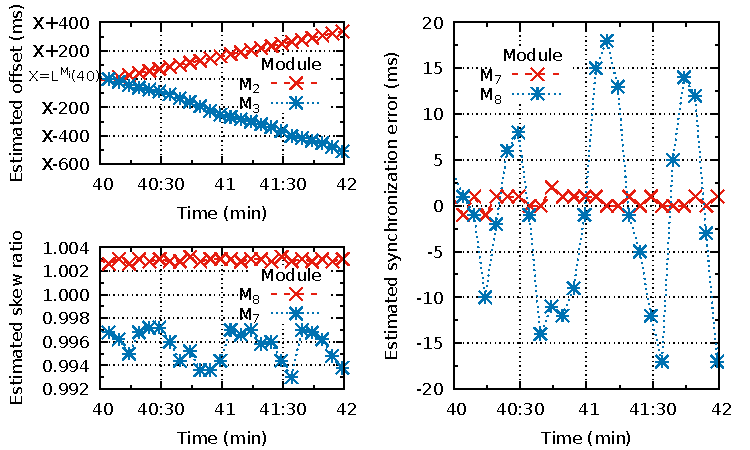
\includegraphics[width=0.7\textwidth]{images/time-synchronization/stability.pdf}
	\end{center}
	\caption{On the left, stability of the local clock of $M_7$ and $M_8$ with respect to the global timescale: above, the estimated offset $(L^{M_i}(40) - \tilde{G}(40) + (L^{M_i}(t) - \tilde{G}(t)))$ and below, the estimation of the estimated average skew ratio between synchronization points $(\frac{\Delta L^{M_i}(t)}{\Delta \tilde{G}(t)})$. On the right, the synchronization error of these two blocks. \label{fig:time-sync:hardware-instability-offset}}
\end{figure}

Since all modules ran under the same experimental conditions, such an important difference in the synchronization precision should be due to the clock oscillator relative stability. Among the dozens of blocks we have, all modules behave similarly to $M_6$, $M_7$, and $M_9$, except for $M_8$. As a consequence, we consider $M_8$ to be an outlier and do not use it in the rest of the experiments. Note that we do not consider $M_8$ to compute our simulation model. We suggest that such outliers should be removed from the system when a precise time synchronization is required.

Furthermore, we experimentally checked that the hop distance to the block that is connected to the power supply has no significant impact on the individual synchronization precision.

\subsubsection{Impact of the Synchronization Periods on the Synchronization Precision}
\label{section:time-sync:eval-period}

Figure~\ref{fig:time-sync:period} shows the impact of the synchronization periods on the relative synchronization error in the doubled L-shaped system depicted in Figure~\ref{fig:time-sync:mrtp-blinkyblocks}. Distributions seem to be Gaussian. They are all bell-shaped and centered around~0. For a runtime synchronization period of 5 seconds, the average  relative synchronization error is equal to 0.22 millisecond.

\begin{figure}[!h]
	\begin{center}
		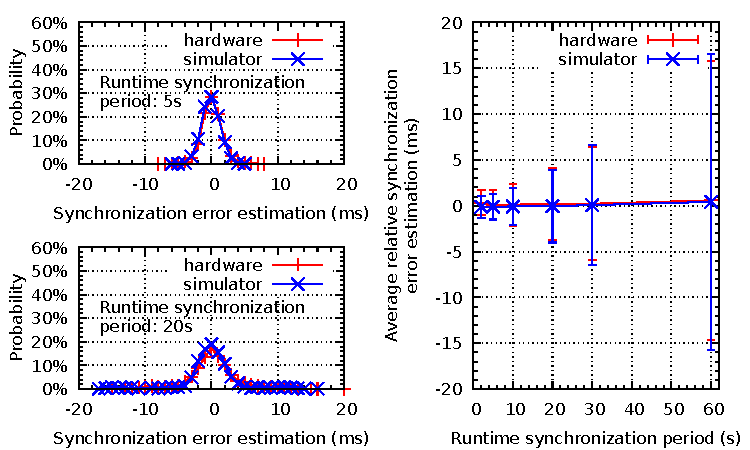
\includegraphics[width=0.75\textwidth,valign=c]{images/time-synchronization/period.pdf}
	\end{center}
	\caption{Relative synchronization error of the whole system as a function of the synchronization periods. On the left, the distribution of the error. On the right, the average error ($\pm$ standard deviation).}
	\label{fig:time-sync:period}
	\label{fig:time-sync:synchronization-error}
\end{figure}

We observe in Figure~\ref{fig:time-sync:period} that the distribution shape becomes shorter and larger, as the runtime synchronization period increases. The error dispersion reflects the synchronization error. The standard deviation increases with the runtime synchronization period. As a consequence, the longer the resynchronization interval is, the worse the synchronization precision will be. However, it must be noted that in all cases, the system stays synchronized to a few milliseconds. The average synchronization error amplitude remains below 4 milliseconds for runtime synchronization periods ranging from 2 seconds to 30 seconds. With a runtime period of 5 seconds, every link of the synchronization tree is theoretically used by MRTP only about 0.12\% of the time during the runtime phase.

\subsubsection{Impact of the Number of Synchronization Points used for the Linear Regressions on the Synchronization Precision}
\label{section:time-sync:eval-window}

Figure~\ref{fig:time-sync:window} shows the impact of the number of synchronization points used for the linear regressions on the synchronization error in the doubled L-shaped system depicted in Figure~\ref{fig:time-sync:mrtp-blinkyblocks}. With a running synchronization period of 5 seconds, we observe that the maximum synchronization precision is obtained using 5 synchronization points for the linear regressions. Indeed, when using 5 synchronization points, the relative synchronization error has a mean close to 0 and the smallest standard deviation. We suppose that the linear regression does not make it possible to properly capture the clock models when using less synchronization points. When using more than five synchronization points, the synchronization precision decreases as the window size increases. We believe, without proving it, that this is because the clock frequencies vary too quickly for a large number of observations.

\begin{figure}[h!]
	\begin{center}
		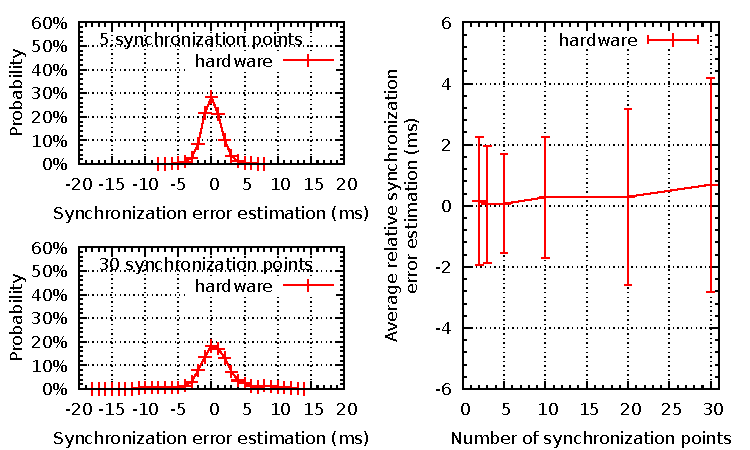
\includegraphics[width=0.75\textwidth]{images/time-synchronization/window.pdf}
	\end{center}
	\caption{Relative synchronization error of the whole system as a function of the number of synchronization points used for the linear regressions. On the left, the distribution of the error. On the right, the average error ($\pm$ standard deviation).\label{fig:time-sync:window}}
\end{figure}

\subsubsection{Simulation Fidelity}

As shown in figures~\ref{fig:time-sync:dissemination-error} and~\ref{fig:time-sync:period}, the results obtained using simulations closely match the results from the hardware-based experiments. Indeed, the results of the simulations have distributions and statistical measure values (i.e., means and standard deviations) that are almost identical to the results of the experiments on hardware systems. The global-time dissemination error according to the hop distance is well simulated even after many hops. Thus, we can safely assume that VisibleSim can be used to study the performance of synchronization protocols on large-scale Blinky Blocks systems.

Note that we do not simulate the experiment in Section~\ref{section:time-sync:eval-window} because we did not compute the processing times for linear regression on a large number of synchronization points (i.e., more than five) in our simulation model.

\subsection{Large-Scale Evaluation and Comparison to Existing Protocols through Simulations}
\label{section:time-sync:large-scale-evaluation}

In this subsection, we use the VisibleSim simulator to evaluate the performance of our protocol and compare it with existing synchronization protocols. Section~\ref{section:time-sync:compared-protocols} presents the synchronization protocols and their variants that we consider for the comparisons.

We study the precision, the convergence time and the communication efficiency of the synchronization protocols on three systems of different sizes and diameters (see Table~\ref{table:time-sync:balls}). These systems are organized in a ball topology, i.e., the largest network topology that can be formed for a given diameter (see Sections~\ref{section:appendixLMRs:model} and~\ref{section:appendixLMRs:diameter-blinkyblocks} for more details). We use this compact network topology because there is an increasing number of modules, therefore an increasing number of clock models, at a given network distance from any given module. Moreover, we consider the ball system composed of 27,775 modules to show that MRTP can effectively synchronize this system to a few milliseconds, as announced in subsection~\ref{section:time-sync:color-changes}.

\begin{table}[h!]
	\small
	\centering
	\begin{tabular}{|c|c|c|c|}
		\hline
		System & Size (modules) & Radius (hops) & Diameter (hops)\\
		\hline
		Ball(5) & 231 & 5 & 10 \\
		\hline
		Ball(15) & 4,991 & 15 & 30 \\
		\hline
		Ball(27) & 27,775 & 27 & 54 \\
		\hline
	\end{tabular}
	\caption{Network characteristics of the systems used for the evaluation of time synchronization protocols.\label{table:time-sync:balls}}
\end{table}

To compare protocols fairly, we evaluate them on identical systems, i.e., for all experiments, a module always has the same position, the same communication model and the same clock parameters. In addition, for centralized protocols, the time master always has the same communication model and clock parameters. Furthermore, the minimum-identifier module is deliberately placed at the extremity of the systems in order to show the impact of the maximum hop distance to the time master on the overall synchronization precision of the system.

All the experiments last for two hours. During the first hour, the system is left unsynchronized. Then, the modules start running one of the considered synchronization protocol. For all the protocols, we use a synchronization period of 5 seconds. In protocols that use a linear model to compensate for clock skew, modules perform the model parameter estimations using the last 5 synchronization points, unless otherwise mentioned. To evaluate the synchronization precision, we measure the maximum pairwise synchronization error every 3 seconds. 

\subsubsection{Compared Synchronization Protocols and Modifications}
\label{section:time-sync:compared-protocols}

We compare MRTP to leading protocols designed for ad-hoc networks, namely MLE\_TPSN (i.e., TPSN~\cite{ganeriwal2003timing} combined with MLE~\cite{leng2010clock}), FTSP~\cite{maroti2004flooding}, PulseSync~\cite{lenzen2009optimal}, WMTS~\cite{he2014time} (a variant of MTS~\cite{he2014time}) and ATS~\cite{schenato2011average}. These protocols were proposed for wireless sensor networks and need modifications to be used on our target platform\footnote{Our implementation of these protocols is available online at: \VisibleSimUrl{}}. This section lists these modifications. Note that the modifications operated do not alter the general high-level framework of the compared protocols.

\paragraph{Communication Medium}

One of the adaptation is to consider a local and wired communication medium instead of a wireless and shared one. The main differences this adaptation causes, from a data-link point of view, are twofold. First, it entails the absence of message loss due to interferences/collisions on the communication medium. Second, in order to broadcast a message to all neighbors, a node has to send an individual copy of that message to all of them.

\paragraph{Communication Delay Compensation} As explained in the state-of-the-art section, the methods used by these protocols to compensate for communication delays are not all directly applicable to our target platform. We recall that three methods are applicable to our target system, namely RTT, FD and PRED (see Section~\ref{section:time-sync:communication-delay-comp-methods}). TPSN is based on RTT. MLE\_TPSN uses round-trip messages and computes the maximum likelihood estimation of the current global time on the last 5 synchronization points.  We use FTSP with PRED because the method proposed in FTSP, which is highly accurate, is not applicable to our target system and because PRED is, on average, the most precise method for our system. PulseSync employs the same method as FTSP, thus we use PulseSync with PRED. In ATS, the authors suggest using the most precise method and utilizing FD for the experimental evaluation. Since PRED is, on average, more precise than FD in our system, we use ATS with PRED. We also use PRED to compensate for communication delays in WMTS.

\paragraph{The ATS and the WMTS Protocols}
ATS and WMTS are respectively average- and maximum-value consensus-based decentralized protocols. WMTS and ATS compensates for clock skew using averaging techniques. In WMTS and in the original version of ATS, modules use the last two clock readings of a neighbor to estimate its relative clock skew. In our modified version of ATS, we use the oldest and the newest clock readings to estimate the relative clock skew. This modification leads to better performance in our system. The ATS protocol takes input parameters, e.g., the probability of updating the clock offset and the clock skew of the modules at each synchronization round. We adopted the parameters used in the evaluation subsection of the original article~\cite{schenato2011average}.

\paragraph{The MRTP and the TPSN Protocols}
MRTP and TPSN are centralized protocols in which modules get periodically synchronized with the time master. In MRTP and TPSN, the time master is elected using an external algorithm and child modules are recursively synchronized by their parents along the edges of a spanning tree. For the leader election problem, we consider two algorithms. To elect the minimum-identifier module, we use the MIN\_ID algorithm that we defined as MIN-ID in Section~\ref{section:centrality:compared-algorithms}. To elect a central node, we use PC2LE-CENTER, the center version of the PC2LE framework introduced in Section~\ref{section:centrality:pc2le}. In the rest of the evaluation section, we use PC2LE to refer to PC2LE-CENTER for conciseness reasons. Table~\ref{table:time-sync:election-performance} shows the performance of these two election algorithms on our target systems. We use the \cheungCb{} algorithm presented in Section~\ref{section:centrality:distributed-primitives} to build the synchronization tree. In~\cite{ganeriwal2003timing}, the author states that any method can be used to select the time master and suggests that the minimum-identifier election algorithm presented in~\cite{malpani2000leader} can be used. Thus, we use TPSN with MIN-ID. In addition, in the original version of TPSN, child modules overhear the messages exchanged during the synchronization process of their parent. As our platform uses contact communications, messages sent to a node cannot be overheard by other nodes. Thus, in our version of TPSN, we added an extra message sent by the parent to trigger the synchronization of child modules. Moreover, the modules use a linear model and MLE~\cite{leng2010clock} to estimate the clock parameters. During a synchronization phase, modules only use the last timing information to disseminate the global time through the system. Without this last modification, MLE\_TPSN diverges slowly in our simulations.

{
	\newcommand{\lenOneTwo}{0.12\linewidth}
	\newcommand{\lenThreeTwo}{0.20\linewidth}
	
	\newcommand{\minId}{MIN\_ID}	
	\newcommand{\pcTwole}{PC2LE}	
	\begin{center}
		\begin{table}[h!]
			\centering
			\small
			\begin{tabular}{|C{\lenOneTwo}|C{\lenOneTwo}|C{\lenThreeTwo}|C{\lenThreeTwo}|C{\lenThreeTwo}|}
				\hline
				System & Algorithms & Simulated execution time (s) & Average number of messages (per module) & Elected-node eccentricity\\
				\hline
				\multirow{2}{*}{Ball(5)} & \minId & 0.25 & 38 &  10\\
				\cline{2-5}
				& \pcTwole & 0.72 & 133 & 5 \\
				\hline
				\multirow{2}{*}{Ball(10)} & \minId & 0.53 & 84 & 30 \\
				\cline{2-5}
				& \pcTwole & 1.96 & 420 & 17 \\
				\hline
				\multirow{2}{*}{Ball(27)} & \minId & 0.83 & 107 & 54 \\
				\cline{2-5}
				& \pcTwole & 3.41 & 735 & 30 \\
				\hline
			\end{tabular}
			\caption{Performance of election algorithms on the systems used for the evaluation of time synchronization protocols.}\label{table:time-sync:election-performance}
		\end{table}
	\end{center}
}

\paragraph{The FTSP and the PulseSync Protcols} FTSP and PulseSync are centralized protocols in which modules get periodically synchronized with the time master. FTSP and PulseSync are infrastructure-less. During the synchronization phases, the minimum-identifier module gets implicitly elected as the time master. If a module has not received new synchronization messages for some synchronization periods (5 in our implementation), it declares itself time master and starts synchronizing the other modules. A module updates its belief concerning the current time master in the system whenever it receives a synchronization message advertising for a time master with a lower identifier. 

In FTSP, a new time master ignores synchronization messages advertising for lower-identifier nodes during 3 synchronization periods. The FTSP protocol also takes as a parameter the number of synchronization messages that a node needs to have received before it considers itself to be synchronized and starts to synchronize neighboring nodes. In our simulations, we use the value of~3. For a better performance, we proceed to the subsequent modifications of FTSP, also suggested in~\cite{lenzen2009optimal}. In the original version of FTSP, synchronized modules ignore the received global time values that are too far from their own estimation of the current global time. As shown in the next subsection, FTSP does not provide precise synchronization in our target system and we had to suppress this filtering procedure in order to obtain better results. Additionally, in our version of FTSP, modules clear their linear regression table whenever they get synchronized by a new time master. 

PulseSync accurately synchronizes nodes using rapid network-wide flooding. Sophisticated methods have been proposed to achieve fast flooding in WSN where messages may interfere and collide with each other (e.g., \cite{ferrari2011efficient}). Our target system does not assume any specific mechanism to quickly disseminate a message through the network. Moreover, Blinky Blocks networks are not prone to message collisions. In our implementation of PulseSync, synchronization messages are handled like any other message. In particular, messages are not prioritized in message queues.

\paragraph{Naming Convention}
We use the following format to name the different approaches compared: {\small\ \ \ [ORIGINAL PROTOCOL NAME]\hyph [LEADER ELECTION ALGORITHM]\hyph [COMMUNICATION DELAY COMPENSATION METHOD]}. For instance, MRTP\hyph PC2LE\hyph PRED refers to the MRTP synchronization protocol based on the PC2LE leader election algorithm and our predictive model to compensate for communication delays.

\subsubsection{Time of Convergence and Achievable Precision}

Figure~\ref{fig:time-sync:error-time-all} shows the average maximum pairwise synchronization error of the modules over time for the compared synchronization protocols. During the first hour, the modules were not synchronized and progressively drifted apart. The system reached a synchronization error of more than 40 seconds.

MRTP, MLE\_TPSN and PulseSync centralized protocols converge in a few seconds in the three systems. We recall that MRTP and MLE\_TPSN first elect a leader, build a spanning tree, and then start synchronizing the modules. In PulseSync, modules wait for 5 synchronization periods (i.e., 25 seconds) without hearing a synchronization message before declaring themselves time masters and trying to synchronize the other nodes. This mechanism causes PulseSync to converge slightly more slowly but makes this protocol inherently tolerant of faults.

As expected, ATS, which is an average consensus-based decentralized protocol, converges much more slowly and the time of convergence significantly increases with the system size. In Ball(15), ATS converges only after about 30~minutes of periodic synchronization. WMTS, which is a maximum-value consensus-based protocol, converges more quickly than ATS. But WMTS is still slightly slower than the MRTP, MLE\_TPSN and PulseSync centralized protocols.

\begin{figure}[h!]
	\centering
	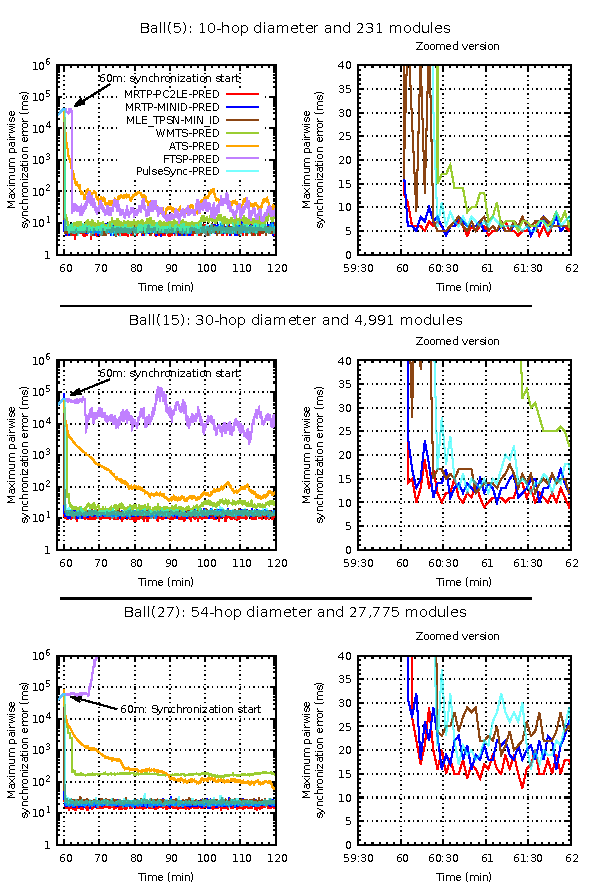
\includegraphics[width=0.93\linewidth]{images/time-synchronization/error-time-all-2x3}
	\caption{Maximum pairwise synchronization error over time. This figure shows both the time of convergence and the achievable precision for each protocol on the different Ball systems.} 
	\label{fig:time-sync:error-time-all}
\end{figure}

\begin{figure}[h!]
	\centering
	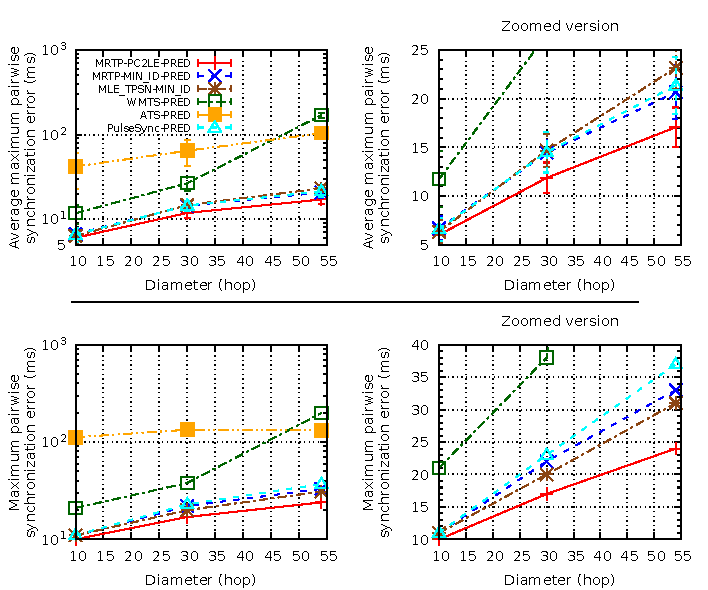
\includegraphics[width=1\linewidth]{images/time-synchronization/precision}
	\caption{Synchronization precision. At the top, average maximum pairwise synchronization error in the last 30 minutes of the experiment ($\pm$ standard deviation). At the bottom, the maximum pairwise synchronization error.}
	\label{fig:time-sync:precision}
\end{figure}

FTSP does not converge in large ensembles of Blinky Blocks. Theoretically, FTSP should have converged in less than 15~minutes in Ball(27)~\cite{maroti2004flooding}. As explained in the related work subsection, the FTSP synchronization waves are slowly flooded through the network using asynchronous broadcasts, whereas in  MRTP, MLE\_TPSN and PulseSync, the current global time gets quickly disseminated throughout the entire network. This last scheme significantly reduces the impact of clock inaccuracies (due to noise, skew variations, time-increasing errors in the local estimation of the global time) on the synchronization precision and the time of convergence.

Figure~\ref{fig:time-sync:precision} shows statistics on the maximum pairwise synchronization error after convergence. Unsurprisingly, the synchronization precision of all the protocols decreases with the network size. MRTP, MLE\_TPSN and PulseSync, which are centralized protocols, have a synchronization precision of a few dozen milliseconds in all the systems considered.

MRTP-PC2LE-PRED is the most precise protocol. As shown in Figure~\ref{fig:time-sync:precision}, using a central node as the time master improves the average maximum pairwise synchronization error of MRTP by about 0.6 to 3.5 milliseconds in the different ball systems (MRTP-PC2LE-PRED vs MRTP-MIN\_ID-PRED). Moreover, the precision improvement increases with the diameter of the ball.

Unsurprisingly, MRTP-MIN\_ID-PRED and PulseSync-PRED have, on average, a similar synchronization precision. It was awaited as the two protocols only differ by the mechanism they use to elect the minimum-identifier node and by their infrastructure (i.e., MRTP uses a breadth-first spanning tree while PulseSync is infrastructure-less and floods the network). However, it must be noted that MRTP-MIN\_ID-PRED has a slightly lower worst-case synchronization error. We did not investigate this point but we suspect this could be due to the fact that, in MRTP, a node always gets synchronized by a message that has traveled on the same and shortest path while in our implementation of PulseSync synchronization messages can come from different and possibly not shortest paths, depending on the network traffic.

MRTP-MIN\_ID-PRED is on average about 2.3 milliseconds more precise than MLE\_TPSN in Ball(27) but has a 2-millisecond higher worst-case synchronization error in both the Ball(15) and Ball(27) systems. We recall that these two protocols only differ by the method they use to compensate for communication delays and clock skew. Moreover, as shown in the next subsection, MRTP with PRED is more communication-efficient than MLE\_TPSN.

As announced in subsection~\ref{section:time-sync:color-changes}, MRTP can effectively synchronize the Ball(27) system, composed of 27,775 modules, to less than 40 milliseconds. Indeed, it synchronizes this system to 17 milliseconds on average and to 24 milliseconds at worst.

As expected, the ATS decentralized method is less precise than the centralized ones. The WMTS decentralized method exhibits similar synchronization precision in Ball(5) to that of the centralized methods, while it fails to accurately synchronize the Ball(27) system.

\subsubsection{Communication Efficiency}
\label{section:time-sync:communication-efficiency}

Figure~\ref{fig:time-sync:messages} shows the average number of messages sent per module and its decomposition according to the message types. We consider three types of message:~the messages due to the leader election process, the ones due to the tree infrastructure creation and the synchronization messages. 

As expected, ATS and WMTS decentralized synchronization protocols use on average more messages per module than the MRTP, MLE\_TPSN and PulseSync centralized protocols. In addition, PulseSync, which uses network-wide floodings, generates on average more messages per module than MRTP and MLE\_TPSN that use a tree-like structure. Thus, the message cost induced by both the leader election process and the infrastructure construction is compensated for in less than one hour.

Let $k$ denote the number of messages used by the compensation delay method ($k = 1$ for PRED and $k = 3$ for round-trip-time-based methods as in MLE\_TPSN). In decentralized methods, $2km$ messages\footnote{Every module sends a synchronization message to all its neighbors.} are sent per synchronization round, while $k(n-1)$ messages\footnote{Every module except the time master gets synchronized by a single node.} are sent in MRTP and MLE\_TPSN, and $2m - (n-1)$ messages\footnote{Every module sends a synchronization message to all its neighbors except to the one from which it got synchronized.} are sent in PulseSync-PRED (after the implicit time-master election has converged). We recall that $n-1 \leq m$ in connected networks. As MLE\_TPSN uses a round-trip time based method, it generates three times more synchronization messages per synchronization phase than MRTP with PRED. In compact systems, the number of links is more important than the number of nodes. Thus, in these systems, PulseSync generates more messages per synchronization round than MRTP with PRED. However, PulseSync is inherently more tolerant of network failures because synchronization waves are flooded through all links and not only along the links of a spanning tree. Thus, if a link fails but the system remains connected, PulseSync may still be able to synchronize all the modules. Nevertheless, in a spanning tree, if a link fails, all the nodes of a sub-tree will not get synchronized.

\begin{figure}[h!]
	\centering
	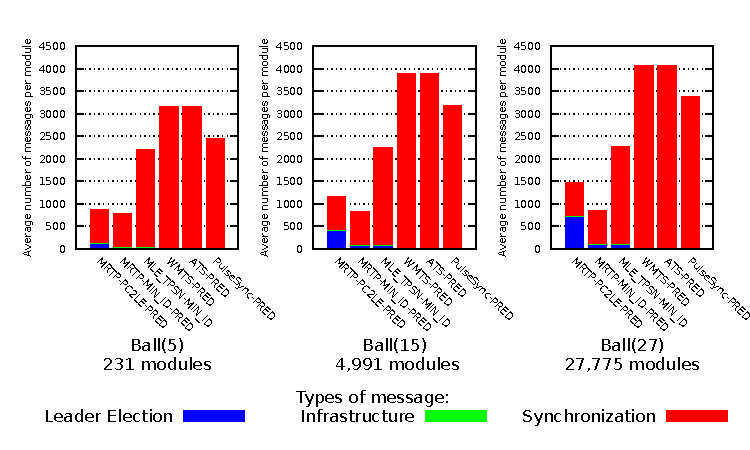
\includegraphics[width=1.0\linewidth]{images/time-synchronization/messages}
	\caption{Average number of messages sent per module in time synchronization protocols.}
	\label{fig:time-sync:messages}
\end{figure}

We measured the maximum message queue size reached by the modules taking into account both the incoming and the outgoing messages. We observed that for any module, the ratio of the maximum queue size reached to the number of neighbors of that module, remains below or equal to three, regardless of the size of the networks for all the protocols, except for PulseSync. For PulseSync, the ratio reached the value of $4.5$. This is due to the uncontrolled-broadcast problem explained in Section~\ref{section:centrality-controlled-broadcast}. This issue does not have a big impact in this case. Indeed, because clocks are drifting apart, nodes trigger synchronization waves at slightly different instants. Thus, neither the leader election process, which involves network-wide flooding(s), nor the actual synchronization phases overwhelm the network. The traffic generated by the synchronization protocols remains well controlled and modules do not require a lot of memory space to store incoming and outgoing messages.

\section{Discussion}

MRTP is intended to synchronize large-scale and fairly stable systems where changes in the network topology, due for instance to module mobility, or potential module or link failures, are infrequent. Our protocol achieves its performance by combining several mechanisms: distributed central-time-master election, fast and recursive propagation of synchronization waves along the edges of a breadth-first spanning tree, low-level timestamping and per-hop compensation for communication delays using the most-appropriate method for the target platform, and clock skew compensation using linear regression.

\paragraph{Design Choices}
In MRTP, a dynamically elected central module periodically synchronizes the system. We assume the network traffic to be evenly distributed in the network. Placing the time master close to the center of the network increases the overall synchronization precision because cumulative errors are made every hop. This strategy is particularly judicious in our context because large-scale modular robots with neighbor-to-neighbor communications tend to exhibit long hop distances. In order to synchronize the system, the time master periodically launches synchronization waves, which are recursively propagated along the edge of a breadth-first spanning tree. Slave modules propagate these waves to their children in the tree shortly after reception. As explained in~\cite{lenzen2009optimal}, optimal synchronization requires a fast propagation scheme. Also note that using a tree is more communication-efficient in compact systems than flooding approaches. Indeed, since there is no broadcast support in the neighbor-to-neighbor communication model, a node has to send an individual copy of a message to all its neighbors in order to broadcast that message. Furthermore, using a breadth-first tree guarantees that synchronization messages always travel on the same and shortest paths. This also leads to better synchronization precision. MRTP performs per-hop synchronization, i.e., a module gets synchronized by a one-hop neighbor. At each hop, the propagated estimation of the current global time is updated to take into account communication delays and time of residence in intermediate modules. Any approach to compensate for these delays can be used in MRTP. Most of the existing approaches use low-level timestamping to suppress the main sources of uncertainty in delay estimations. The best-suited technique to be actually used in MRTP depends on the target platform (i.e., the clock precision, its resolution, the communication mechanism and the network load) and should be carefully selected, since it has a direct impact on the performance of our protocol, both in terms of precision and communication efficiency. We provided a method to experimentally evaluate the precision of a given approach over multiple hops.

\paragraph{Network Density}
We showed that, with a central time master, MRTP can synchronize the 54-hop-diameter ball system composed of 27,775 modules to 24 milliseconds, at worst. In Section~\ref{section:centrality:centers:applications}, we showed that MRTP can synchronize a sparser 83-hop-diameter system, composed of 1,456 nodes, to 29 milliseconds, at worst, when the time master is placed at the center of the system. These worst-case synchronization errors (i.e., the maximum value over all the maximum pairwise synchronization error values that were captured every 3 seconds) are consistent with each other. However, we observed that the averaged maximum pairwise synchronization error is smaller on the sparser system (13 milliseconds versus 17 milliseconds), although it exhibits a larger diameter. We did not investigate this phenomenon, but we believe this is because bad cases happen more rarely in the sparser system, in part because there are less nodes and less long independent paths in that system. Indeed, nodes that receive synchronization messages that have traveled on long and almost independent paths, causing the error accumulated at every hop to be propagated differently, tend to exhibit a high maximum pairwise synchronization error. 

Moreover, it must be noted that, on the Blinky Blocks, the number of simultaneous communications impacts the transfer time (see Section~\ref{section:time-sync:communication-properties}). Thus,   methods of compensating for communication delays may exhibit a different precision depending on the network density, as shown in Section~\ref{section:time-sync:delay-comp-method}. Hence, the achievable synchronization precision may differ depending on the network density.

\paragraph{Portability}
Our protocol is portable to any modular robot system where modules interact together using only neighbor-to-neighbor communications even if their internal clocks are low precision and have high skew relative to one another. Depending on the time master election procedure, it may also be required that every module has a unique identifier. We evaluated MRTP on the Blinky Blocks platform, which is equipped with a very low-accuracy and poor-resolution clock, but it must be noted that our protocol can also be used in systems with more precise clocks. It will indeed have two main effects. First, a lower resolution will lead to more precise local clock readings, i.e., more precise message timestamps. Hence, communication delays may be more precisely captured and compensated for, using potentially a different method than the predictive one we use with the Blinky Blocks. Second, a more precise clock implies reduced clock skew, drift (variation of skew) and noise. This can only increase our protocol precision. It must be noted that, even with higher-precision clocks, it is still appropriate to use a linear model to compensate for short-term clock skew. Indeed, this approach is also commonly used in systems equipped with more precise clocks (e.g., RBS~\cite{elson2002fine}, FTSP~\cite{maroti2004flooding}, PulseSync~\cite{lenzen2015pulsesync}, etc.). Consequently, our protocol should also be able to efficiently synchronize systems equipped with higher-precision clocks. We let the evaluation of our protocol in such systems for future works.

\section{Conclusion}
\label{section:time-sync:conclusion}

In this chapter, we described the Modular Robot Time Protocol (MRTP), a network-wide time synchronization protocol for modular robots. We evaluated our protocol on the Blinky Blocks platform, both on hardware and through simulations. We showed that MRTP can potentially manage systems composed of up to 27,775 Blinky Blocks. Furthermore, the experimental results show that MRTP is able to successfully maintain a Blinky Blocks system synchronized to a few milliseconds, using few network resources at runtime, although the Blinky Blocks are equipped with very low-accuracy and poor-resolution clocks. Simulations results show that MRTP exhibits on average a lower maximum pairwise synchronization error than the compared protocols, while sending more than half less messages in compact systems.
%half the amount of messages or even less